%-------------------------------------------------------------------------------
%	PACKAGES AND OTHER DOCUMENT CONFIGURATIONS
%-------------------------------------------------------------------------------

\documentclass[12pt,a4paper]{tufte-book}
\hypersetup{colorlinks}
\usepackage{microtype}
\usepackage{lipsum}
\usepackage{booktabs}
\usepackage{graphicx}
\graphicspath{{graphics/}}
\setkeys{Gin}{width=\linewidth,totalheight=\textheight,keepaspectratio}
\usepackage{fancyvrb}
\fvset{fontsize=\normalsize}
\newcommand{\hangp}[1]{\makebox[0pt][r]{(}#1\makebox[0pt][l]{)}}
\newcommand{\hangstar}{\makebox[0pt][l]{*}}
\usepackage{xspace}
\newcommand{\monthyear}{\ifcase\month\or January\or February\or March\or April\or May\or June\or July\or August\or September\or October\or November\or December\fi\space\number\year} 
\newcommand{\openepigraph}[2]{
	\begin{fullwidth}
	\sffamily\large
	\begin{doublespace}
	\noindent\allcaps{#1}\\
	\noindent\allcaps{#2}
	\end{doublespace}
	\end{fullwidth}
}

\newcommand{\blankpage}{\newpage\hbox{}\thispagestyle{empty}\newpage}
\usepackage{units}
\newcommand{\hlred}[1]{\textcolor{Maroon}{#1}}
\newcommand{\hangleft}[1]{\makebox[0pt][r]{#1}}
\newcommand{\hairsp}{\hspace{1pt}}
\newcommand{\ie}{\textit{i.\hairsp{}e.}\xspace}
\newcommand{\eg}{\textit{e.\hairsp{}g.}\xspace}
\newcommand{\na}{\quad--}
\newcommand{\measure}[3]{#1/#2$\times$\unit[#3]{pc}}
\newcommand{\tuftebs}{\symbol{'134}}
\providecommand{\XeLaTeX}{X\lower.5ex\hbox{\kern-0.15em\reflectbox{E}}\kern-0.1em\LaTeX}
\newcommand{\tXeLaTeX}{\XeLaTeX\index{XeLaTeX@\protect\XeLaTeX}}
\newcommand{\doccmdnoindex}[2][]{\texttt{\tuftebs#2}}

\newcommand{\doccmddef}[2][]{\hlred{\texttt{\tuftebs#2}}\label{cmd:#2}\ifthenelse{
	\isempty{#1} }{
	\index{#2 command@\protect\hangleft{\texttt{\tuftebs}}\texttt{#2}} } {
	\index{#2 command@\protect\hangleft{\texttt{\tuftebs}}\texttt{#2} (\texttt{#1} package)}
	\index{#1 package@\texttt{#1} package}\index{packages!#1@\texttt{#1}}}
}

\newcommand{\doccmd}[2][]{ \texttt{\tuftebs#2} \ifthenelse{\isempty{#1}} {
	\index{#2 command@\protect\hangleft{\texttt{\tuftebs}}\texttt{#2}} } {
	\index{#2 command@\protect\hangleft{\texttt{\tuftebs}}\texttt{#2} (\texttt{#1} package)}
	\index{#1 package@\texttt{#1} package}\index{packages!#1@\texttt{#1}} }
}

\newcommand{\docopt}[1]{\ensuremath{\langle}\textrm{\textit{#1}}\ensuremath{\rangle}}
\newcommand{\docarg}[1]{\textrm{\textit{#1}}}
\newenvironment{docspec}{\begin{quotation}\ttfamily\parskip0pt\parindent0pt\ignorespaces}{\end{quotation}}
\newcommand{\docenv}[1]{\texttt{#1}\index{#1 environment@\texttt{#1} environment}\index{environments!#1@\texttt{#1}}}
\newcommand{\docenvdef}[1]{\hlred{\texttt{#1}}\label{env:#1}\index{#1 environment@\texttt{#1} environment}\index{environments!#1@\texttt{#1}}}
\newcommand{\docpkg}[1]{\texttt{#1}\index{#1 package@\texttt{#1} package}\index{packages!#1@\texttt{#1}}}
\newcommand{\doccls}[1]{\texttt{#1}}
\newcommand{\docclsopt}[1]{\texttt{#1}\index{#1 class option@\texttt{#1} class option}\index{class options!#1@\texttt{#1}}}
\newcommand{\docclsoptdef}[1]{\hlred{\texttt{#1}}\label{clsopt:#1}\index{#1 class option@\texttt{#1} class option}\index{class options!#1@\texttt{#1}}}
\newcommand{\docmsg}[2]{\bigskip\begin{fullwidth}\noindent\ttfamily#1\end{fullwidth}\medskip\par\noindent#2}
\newcommand{\docfilehook}[2]{\texttt{#1}\index{file hooks!#2}\index{#1@\texttt{#1}}}
\newcommand{\doccounter}[1]{\texttt{#1}\index{#1 counter@\texttt{#1} counter}}

\usepackage{makeidx}
\makeindex

\newcommand{\vdqi}{\textit{VDQI}\xspace}
\newcommand{\ei}{\textit{EI}\xspace}
\newcommand{\ve}{\textit{VE}\xspace}
\newcommand{\be}{\textit{BE}\xspace}
\newcommand{\VDQI}{\textit{The Visual Display of Quantitative Information}\xspace}
\newcommand{\EI}{\textit{Envisioning Information}\xspace}
\newcommand{\VE}{\textit{Visual Explanations}\xspace}
\newcommand{\BE}{\textit{Beautiful Evidence}\xspace}
\newcommand{\TL}{Tufte-\LaTeX\xspace}

\geometry{
  left=24.8mm,
  textwidth=120mm,
  marginparsep=8.2mm,
  marginparwidth=35.4mm
}

%----------------------------------------------------------------------------------------
%	BOOK META-INFORMATION
%----------------------------------------------------------------------------------------

\title{Estimating Activity From Passively Collected Data}
\newcommand{\subtitle}{A Case Study of Smart Street Sensor Project}
\author[Balamurugan Soundararaj]{Balamurugan Soundararaj}
\publisher{University College London}
\begin{document}
\frontmatter

%-------------------------------------------------------------------------------
%	EPIGRAPH - Three good quotes about the research
%-------------------------------------------------------------------------------

\thispagestyle{empty}
\openepigraph{There is no logic that can be superimposed on the city; people make it, and it is to them, not buildings, that we must fit our plans.}{Jane Jacobs,{ \small \itshape The Death and Life of Great American Cities}}
\vfill
\openepigraph{Information is the oil of the 21st century, and analytics is the combustion engine}{Peter Sondergaard,{\small \itshape SVP, Gartner}}
\vfill
\openepigraph{Errors using inadequate data are much less than those using no data at all}{Charles Babbage {\small \itshape The Education Industry}}
\maketitle

%-------------------------------------------------------------------------------
%	Declaration Page
%-------------------------------------------------------------------------------

\newpage
\begin{fullwidth}
~\vfill
\thispagestyle{empty}
\setlength{\parindent}{0pt}
\setlength{\parskip}{\baselineskip}
% \copyright\ \the\year,\ \thanklessauthor\\
\smallcaps{Doctor of Philosophy}\\
\smallcaps{Department of Geography, UCL}
  \par I, \textit{Balamurugan Soundararaj} confirm that the work presented in this thesis is my own. Where information has been derived from other sources, I confirm that this has been indicated in the thesis.\index{declaration}\\
  \vspace{1cm}
  \par..........................................................................
\par\textit{Submitted on, \monthyear}
\end{fullwidth}

%-------------------------------------------------------------------------------
%	FRONT MATTER
%-------------------------------------------------------------------------------
% \setcounter{secnumdepth}{1}
% \setcounter{tocdepth}{1}
\tableofcontents
\listoffigures 
\listoftables

%-------------------------------------------------------------------------------
%	Chapters
%-------------------------------------------------------------------------------

%-------------------------------------------------------------------------------
%	EPIGRAPH - Three good quotes about the research
%-------------------------------------------------------------------------------

\thispagestyle{empty}

\openepigraph{There is no logic that can be superimposed on the city; people make it, and it is to them, not buildings, that we must fit our plans.}{Jane Jacobs,{ \small \itshape The Death and Life of Great American Cities}}
\vfill

\openepigraph{Information is the oil of the 21st century, and analytics is the combustion engine}{Peter Sondergaard,{\small \itshape SVP, Gartner}}
\vfill

\openepigraph{Errors using inadequate data are much less than those using no data at all}{Charles Babbage {\small \itshape The Education Industry}}
\maketitle

%-------------------------------------------------------------------------------
%	Declaration Page - as per UCL regulations
%-------------------------------------------------------------------------------

\newpage
\begin{fullwidth}
~\vfill
\thispagestyle{empty}
\setlength{\parindent}{0pt}
\setlength{\parskip}{\baselineskip}
\smallcaps{Doctor of Philosophy}\\
\smallcaps{Department of Geography, UCL}
\par I, \textit{Balamurugan Soundararaj} confirm that the work presented in this thesis is my own. Where information has been derived from other sources, I confirm that this has been indicated in the thesis.\index{declaration}\\
\vspace{1cm}
\par..........................................................................
\par\textit{Submitted on, \monthyear}
\end{fullwidth}


%-------------------------------------------------------------------------------
%	Dedication
%-------------------------------------------------------------------------------

\cleardoublepage
~\vfill
\begin{doublespace}
\noindent\fontsize{12}{12}\selectfont\itshape \nohyphenation
\hspace{4cm}Dedicated to my parents,

\hspace{3.5cm}S. Kalavathy and K. Soundararaj.
\end{doublespace}
\vfill
\vfill

%-------------------------------------------------------------------------------
%	Table and Lists of Content
%-------------------------------------------------------------------------------

\setcounter{secnumdepth}{2}
\setcounter{tocdepth}{1}
\tableofcontents
\listoffigures 
\listoftables

%-------------------------------------------------------------------------------
\chapter*{Glossary} \label{front:glossary}
%-------------------------------------------------------------------------------

\begin{itemize}
  \item \textbf{Active vs Passive Collection} - Active collection is where the data collection process involves the active participation from the study subjects. In passive data collection, no such participation is required. For example, a web form based survey is an active data collection process while a script collecting data on user's data on a website is passive. This shall not be confused with primary and secondary data where the difference is mainly due to who collects the data from the source.

  \item \textbf{Anonymisation and Pseudonymisation } - The act of removing personal or identifiable information from the data. For example, removing the names and date of birth of people in a dataset. Anonymisation could be carried out in various ways two most popular approaches are generalisation and perturbation. Pseudonymisation is similar but the personally identifiable data is substituted with artificial identifier. The difference between them is that in anonymisation the personal information is permanently purged and there is no way of getting the information back. De-anonymisation is the reverse process of getting personal identifiable data from anonymised data.
    
  \item \textbf{Big Data} - Generally defined as data which could not be handled with regularly used tools and techniques. There are more nuanced definitions of big data depending on the dimension, context and industry. These concepts are discussed in detail in Section \ref{section:toolkit}.

  \item \textbf{Bluetooth} - Short wavelength, low energy, short range wireless technology used for transferring data between electronic devices. They are generally used by mobile devices to connect to peripherals. 

  \item \textbf{CDRC} - The Consumer Data Research Center is an investment from Economic Social Research Center, UK for working with consumer-related organisations to open up their data resources to trusted researchers thus enabling them to carry out important social and economic research.

  \item \textbf{Cellular/Mobile Network} - Terrestrial, long range and wireless network which provides connectivity to mobile devices embedded in them. Most commonly used to denote the networks that provides telephony and internet services to mobile devices using radio waves. 

  \item \textbf{Cryptographic Hashing} - This is the process of transforming a variable set of characters or contents of a file into a fixed length string (checksum). The process is usually one way and is not reversible without a rainbow attack using a database of checksums of all possible values. This is generally used for storing user passwords and to verify the integrity/ authenticity of data. In this thesis hashing functions are used for the purpose of anonymisaiton 

  \item \textbf{Data Partner} - Local Data Company - the organisation which developed the Smart Street Sensor project in conjunction with CDRC. The organisation is solely responsible for the design, manufacture, installation and maintenance of the Smart Street Sensors.

  \item \textbf{Device Fingerprinting} - This is the process of identifying devices through forensic analysis. This commonly used to identify users from data collected by operational websites. This commonly done through identifying unique configurations of the devices such as screen sizes, versions of software installed, etc. In this thesis fingerprinting is used to denote such processes where unique devices are identified from randomised data.

  \item \textbf{Encryption} - This is the process of converting a information into unintelligible format using an algorithm (cipher) to prevent unauthorised access. The process is two way since the resulting cipher-text can be decrypted to restore information. The most common methods used is a public-key based encryption scheme known as 'Diffie Hellman key exchange'.
    
  \item \textbf{Footfall} - Number of people at a given location at a give time. In this thesis the term is used synonymous to footfall at a high street - which is only the pedestrians walking along the particular sidewalk of the high street and does not include people on the carriage way in vehicles.

  \item \textbf{High Street} - The primary business street in a town or a local area where most shops and commercial activity are located. This term is often used to contrast and distinguish from 'Shopping centers' which are large designated areas earmarked for retail activity exclusively.
    
  \item \textbf{Localisation} - Though localisation could mean both GSM localisation and indoor positioning where the location of a device is indirectly derived from other information, in this thesis localisation is used mainly in the context of indoor positioning of mobile devices using techniques other than GPS. The localisation of objects is often relative to each other or to an object with an established position.
    
  \item \textbf{Location, Sensor and Install} - In this thesis and the Smart Street Sensor project, 'location' refers to a physical or geographic location in United Kingdom, 'sensor' denotes the electronic equipment used to collect data and 'install' refers to the time when a particular sensor was operating from a particular location.
    
  \item \textbf{Mobile Device} - A portable computing device such as a smartphone or tablet computer. This also includes wearables and other devices which have computing hardware and can operate independently of another device.
    
  \item \textbf{Personally Identifiable Information} - Any data that could potentially identify a specific individual. Any information that can be used to distinguish one person from another and can be used for de-anonymizing anonymous data can be considered personally identifiable information. In this thesis, the Media Access Control address is considered as sensitive personally identifiable information. 
    
  \item \textbf{Positioning} - Positioning is the measurement of the absolute position (coordinates) of an object with reference to the earth. This is usually achieved through the use of Global Positioning System or similar systems.

  \item \textbf{Probe Request} - This is a special signal broadcast by Wi-Fi enabled mobile devices to elicit a response (probe response) from Wi-Fi access points which can receive them. The primary purpose of the probe request is to enumerate the available Wi-Fi networks and there can also be secondary purposes such as indoor positioning.

  \item \textbf{Real-time} - This is highly subjective concept which could be defined as the phenomena which occurs sufficiently immediately. In this thesis real-time is used to describe data which is collected within an hour after the event has occurred.

  \item \textbf{Sensor Configuration} - The way the sensor is installed at a particular location. This includes the this includes the position of the sensor in terms of height and depth, the material of shopfront etc.

  \item \textbf{Signal, Noise} - 'Signal' is used to denote the data received from devices which are within study area and 'Noise' to denote the data from devices outside the study area.

  \item \textbf{Smart Street Sensor Project} - This project is a comprehensive study of live footfall patterns across Great Britain using 1,000 Wi-Fi based sensors located in high streets across 81 towns and cities across the country. Smart Street Sensor is a Raspberry Pi based sensor designed and manufactured by the Data partner which collects data for the project.

  \item \textbf{Wi-Fi} - A family of medium range radio technologies based on the IEEE 802.11 family of standards which are generally used for wireless local area networking between devices.

\end{itemize}

%-------------------------------------------------------------------------------
%	Outputs from Research
%-------------------------------------------------------------------------------

\chapter*{Outputs From The Research} \label{front:outputs}

\section*{Publications}
\textbf{Book Chapter} - Murcio, R., Soundararaj, B., \& Lugomer, K. (2018). Movements in Cities: Footfall and its Spatio-Temporal Distribution. In Longley P., Cheshire J., \& Singleton A. (Authors), \textit{Consumer Data Research} (pp. 84-95). London: UCL Press.
\vspace{0.2cm} \par \noindent \textbf{Journal Paper} - Soundararaj, B., Cheshire, J., \& Longley, P. (2019) Estimating real-time high-street footfall from Wi-Fi probe requests, \textit{International Journal of Geographical Information Science}.
\vspace{0.2cm} \par \noindent \textbf{Conference Paper} - Soundararaj, B., Cheshire, J., \& Longley, P. (2019). Medium Data Toolkit - A Case study on Smart Street Sensor Project. \textit{In Proceedings of GIS Research UK}, New Castle, United Kingdom.
\vspace{0.2cm} \par \noindent \textbf{Conference Paper} - Lugomer, K., Soundararaj, B., Murcio, R., Cheshire, J., \& Longley, P. (2017). Understanding sources of measurement error in the Wi-Fi sensor data in the Smart City. \textit{In Proceedings of GIS Research UK}, Manchester, United Kingdom.
\vspace{0.2cm} \par \noindent \textbf{Conference Paper} - Soundararaj, B., \& Zhu, D. (2019). Estimating pedestrian flow from footfall counts using Geo-propagation. \textit{In Proceedings of Conference on Complex Systems}, Singapore\sidenote{\textit{Under consideration}}.
\vspace{0.2cm} \par \noindent \textbf{Conference Paper} - Murcio, R., Soundararaj, B., \& Lugomer, K. (2018). Trends in urban flows: An information theory approach. \textit{In Proceedings of Conference on Complex Systems}, Cancun, Mexico.
\vspace{0.2cm} \par \noindent \textbf{Conference Paper} - Soundararaj, B., Murcio, R., \& Lugomer, K. (2016). Smart Street Sensor Footfall Project. \textit{In Proceedings of Conference on Complex Systems}, Amsterdam, Netherlands.
\vspace{0.2cm} \par \noindent \textbf{Conference Paper} - Soundararaj, B., \& Lugomer, K. (2016). Smart Street Sensor Footfall Project. \textit{In Proceedings of Oxford Retail Futures Conference}, Oxford, United Kingdom.

\section*{Engagement Activities}
\vspace{0.2cm} \par \noindent \textbf{Event Talk} - Estimating real-time high street footfall from Wi-Fi probe requests. (2018). \textit{Geo+data}, London, United Kingdom.
\vspace{0.2cm} \par \noindent \textbf{Event Talk} - Estimating real-time high street footfall from Wi-Fi probe requests. (2018). \textit{Data Natives}, London, United Kingdom.
\vspace{0.2cm} \par \noindent \textbf{Conference Workshop} - Estimating real-time high street footfall from Wi-Fi probe requests. (2018). \textit{Smart Urban Policy Futures Workshop}, London, United Kingdom.
\vspace{0.2cm} \par \noindent \textbf{Exhibition} - Real-time footfall in Bloomsbury. (2017). \textit{big data Here - big data Week 2016}, London, United Kingdom.

\section*{Products}
\vspace{0.2cm} \par \noindent \textbf{Research Dataset} - Smart Street Sensor footfall data, \textit{Consumer Data Research Center}. URL: \url{https://data.cdrc.ac.uk}.
\vspace{0.2cm} \par \noindent \textbf{Software} - Soundararaj, B. (2018). Clicker - an Android app for manually counting pedestrian footfalls with precision and accuracy. \textit{Google Play Store}. URL: \url{https://play.google.com/store/apps?id=com. bala. manualcount}.

\section*{Awards}
\vspace{0.2cm} \par \noindent \textbf{Best Paper} - Early Career Research paper at \textit{GIS Research UK conference, New Castle} (2019).
\vspace{0.2cm} \par \noindent \textbf{Bursary} - Yusuf Ali travel bursary (2017) \textit{University College London}.


%===============================================================================
\chapter*{Prologue}
%===============================================================================

%-------------------------------------------------------------------------------
\section*{Abstract} 
%-------------------------------------------------------------------------------

Measuring the distribution and dynamics of the population at granular level both spatially and temporally is crucial for understanding the structure and function of the built environment.
In this era of big data, there have been numerous attempts to undertake this using the preponderance of unstructured, passive and incidental digital data which are generated from day-to-day human activities.
In attempts to collect, analyse and link these widely available datasets at a massive scale, it is easy to put the privacy of the study subjects at risk.

This research looks at one such data source - Wi-Fi probe requests generated by mobile devices - in detail, and processes it into granular, long-term information on number of people on the retail high streets of the United Kingdom (UK).
Though this is not the first study to use this data source, the thesis specifically targets and tackles the uncertainties introduced in recent years by the implementation of features designed to protect the privacy of the users of Wi-Fi enabled mobile devices.
This research starts with the design and implementation of multiple experiments to examine Wi-Fi probe requests in detail, then later describes the development of a data collection methodology to collect multiple sets of probe requests at locations across London.
The thesis also details the uses of these datasets, along with the massive dataset generated by the \textit{`Smart Street Sensor'} project, to devise novel data cleaning and processing methodologies which result in the generation of a high quality dataset which describes the volume of people on UK retail high streets with a granularity of 5 minute intervals since August 2015 across 1000 locations (approx.) in 115 towns.

This thesis also describes the compilation of a bespoke \textit{`Medium data toolkit'} for processing Wi-Fi probe requests (or indeed any other data with a similar size and complexity).
Finally, the thesis demonstrates the value and possible applications of such footfall information through a series of case studies.
By successfully avoiding the use of any personally identifiable information, the research undertaken for this thesis also demonstrates that it is feasible to prioritise the privacy of users while still deriving detailed and meaningful insights from the data generated by the users.

%-------------------------------------------------------------------------------
\section*{Impact Statement}
%-------------------------------------------------------------------------------
We live in the age of data deluge where data are generated at a pace that far exceeds our capacity to digest and analyse them.
Putting these amounts of data to use within the constraints of available resources and time, is one of the biggest challenges faced by researchers today.
The primary impact of this research is in solving this issue.
This research utilised one such dataset - Wi-Fi signals generated by millions of mobile phones all around the year and available to anyone with a Wi-Fi receiver - then cleaned and processed them into highly granular and longitudinal information on the volume of footfall at retail high streets across the UK.

In  converting the unstructured data into useful information, the research undertaken for this thesis developed two novel methods - one for filtering Wi-Fi signals based on their strength, and the other for grouping them based on their source mobile device.
Moreover, this was achieved without revealing the identity of the users.
These techniques enable researchers to deal with datasets exhibiting similar challenges such as Bluetooth signals, or records of people's clicking as they navigate through websites, etc.
These methodologies and their results have been published in a peer reviewed journal \textit{International Journal for Geographic Information Science} for the benefit of the wider community.
They were also presented to the data partner who collaborated with the research unit - \textit{Consumer Data Research Centre (CDRC)} - for the Smart Street Sensor project, and were considered for inclusion in the data partner's commercial project.

When dealing with the large and complex Wi-Fi dataset, the research designed and implemented a bespoke toolkit and a data processing pipeline comprising of open-source and free software which could be used by other researchers for use with similar datasets.
The work on  this `Medium-data toolkit' was presented at the conference \textit{Geographic Information Science Research UK}.
Moreover the research directly led to the creation and maintenance of the \textit{aggregated footfall} data product disseminated by CDRC\sidenote[][-2cm]{\textit{Local Data Company \& UCL Smart Street Sensor Footfall Data: Research Aggregated data - \url{https://bit.ly/2FNGmo0}}}, and has served as the data source for multiple research projects within and outside CDRC and UCL.

Apart from the technical impact, the primary output of the research - footfall volumes on retail locations - has commercial and policy impact for all the stakeholders involved with the retail industry in the UK.
From this information comes a variety of insights: retailers can derive insights on the patterns of customer movement around their shops; landlords can find a reliable way to value their properties; local authorities gain a way to quantify and track the vibrancy of their retail centres over long periods of time; and consumers get information on which areas might be crowded at any given time.
Finally, in the past 3 years, the outputs from this research have been disseminated to the broader academic community and industry through a series of paper presentations at conferences such as \textit{GIS Research UK} and \textit{Conference of Complex Systems}, talks at \textit{Data natives}, \textit{Geo+Data London}, and \textit{Smart Urban Policy Futures Workshop}, industry events such as \textit{Oxford Retail Futures Conference}, and public engagement events such as the \textit{big data Here} exhibition.

%-------------------------------------------------------------------------------
\section*{Acknowledgements} 
%-------------------------------------------------------------------------------

I would like to thank my supervisors James Cheshire and Paul Longley for their guidance, support and relentless motivation.
I am deeply grateful to my family who have supported me through my academic journey to whom I owe everything I have ever achieved.
A very special gratitude goes to Anshita whose unwavering support and understanding got me through the most stressful times of my research.
My sincere thanks to all my friends and colleagues from \textit{Consumer Data Research Center} and \textit{Department of Geography, UCL} who have helped me in the research.
Most of the data collection carried out in this research were made possible by the help and support from our data partner - \textit{Local Data Company}.
I would like to thank \textit{Economic and Social Research Council} for funding the research under the awards - ES/L011840/1 and 1625064.
Last but not the least, I would like to thank the contributors to all the open source and free projects I have used in this research (appendix \ref{appendix:software}). I am forever indebted to them and hope to repay them by contributing back to the community for the rest of my career.

\cleardoublepage
\chapter{Introduction}


We talk about the theory of cities and built environment. We start from how
these have been perceived as function of the form and gradually changed to
people, activity, economy and information. Built environment is manifestation of
information exchange that happens in them. We talk about the change in theory
regarding this. We talk about how this information exchange has been becoming
more and more open and the opportunity it provides us planners, geographers and
researchers to understand these things better.

Along with the information age there is an explosion of open data. The data
collection has changed from structured high effort activity to low effort
scraping activity. The data generated by scraping is unprecedented and
staggering. Most of the Big-data research has gone into this in the past decade.
Disadvantages of structured data which the unstructured data fills. This is
changing how we view, understand and experience the world. Some of these
datasets fall into this unique medium size category as well which are neither
big data nor trivial. There is a need for methods and tools to collect, convert
and use these data.

Talk about the ubiquity of the mobile technology. Everyone has a device which
connects them with world wirelessly. Major ones cellphone and Wi-Fi Wi-Fi is
uniquely placed in between Cellphone and Bluetooth. The design of Wi-Fi gives us
amazing opportunity. This has been done before for the past decade by loads. The
privacy advocacy has become a new thing. The change is from both ends.
Collectors are regulated, cellphones are getting sneakier. Need for method to
collect data and analyse it without compromising on privacy. The conversion of
this unstructured data into something tangible and measurable is not a trivial
problem \cite{gandomi2015beyond}. There are loads of such data and measurements. Examples - banking vs
economic activity, oyster card data vs movement.

The potential use of such information is immense. Give examples of smart city
paradigm and connected city where real time census is possible. We can not only
take snapshot of the state of the city, we can record and understand the built
environment as living, breathing organism. The insights we get by combining this
information with other similar info is more than sum of their parts. It can
revolutionise understanding , planning, policy etc, urban management and finally
industry such as retail, transportation etc. city mapper, sharing economy etc.

\cleardoublepage
%===============================================================================%
\chapter{Review of Literature}\label{chapter:literature}
%===============================================================================%

Understanding the scale, nature and dynamics of distribution of population across space and time has been the central premise of academic research in various fields of study such as human geography, sociology, transportation, urban planning and managements.
This granular knowledge of where people are and how they move is also critical in practical decision making in various industries such as real estate for valuing places, retail for business planning and risk management during emergencies for evacuation.
The primary challenge faced by any research concerning the population at this scale is the collection of precise and accurate data in a timely manner.
Though large structured datasets such as national census provides comprehensive coverage they are sparse temporally and understanding dynamics of population withing shorter periods is not possible.
Alternatively, smaller datasets such as sample surveys and traffic counts are collected more frequently they are not comprehensive enough. 
This pursuit for identifying a data source which has the best features of both type of datasets started as an inquiry into methods to estimate and interpolate highly granular data from existing regional level aggregate data.
As technology improved through the later half of twentieth century, research methodologies adopted the new tools and technologies to not only improve the quality of estimations but also to collect data with high granularity.
Though new technologies provided immense opportunity in collecting large amounts of data which were previously impossible, they also introduced their own share of uncertainties.
Hence it becomes imperative that we understand the evolution of these techniques and methodologies along with the research that used them to build our rationale behind any further research.
Moreover with the proliferation of mobile devices and wireless internet connectivity, every day to day activity is being digitised leading to the creation of large amount of easily accessible data which are generated passively in an unstructured manner.
The users' acceptance to the collection and analysis of such data has also been improving until recently \cite{kobsa2014}.
There has also been rising concerns regarding user privacy along with the development of more accurate methods to track them.
In this context, the critical task in all these research is to solve the problem of balancing these two - collecting relevant data and protecting user privacy, by choosing the right technologies and devising the appropriate methods.

In this chapter a systematic survey of literature in the broad multidisciplinary area of research - `distribution and dynamics of human activity' has been conducted.
The aim of this survey was to evaluate the stage at which the research is currently at, understand its evolution and progress through time and identify the possibilities that exists for future research.
A comprehensive survey of over 300 publications which discuss this area of research was undertaken covering the major themes and trends in the last 70 years.
These themes were discussed in detail to outline what has been achieved in the corresponding fields of study highlighting the opportunities and gaps in research that still exist.
The timeline of publication of these research has also been studied to discuss the evolution of the research along with the changes in the technology landscape.
These studies were then classified in terms of the major technologies employed by them to uncover the trends in how various technologies have been adopted and phasing out during this period.
The primary objective was to understand the advantages and disadvantages of these techniques and to develop a theoretical framework for understanding when and how to use them effectively to answer research questions.
Finally the literature survey was summarised focussing on the major research gaps that still exist and interesting new areas of research that has emerged recently  where more research is warranted.
These areas of research were also critically evaluated in terms of priority and feasibility leading to the development of questions and plan for this research thesis. 

\begin{marginfigure}
  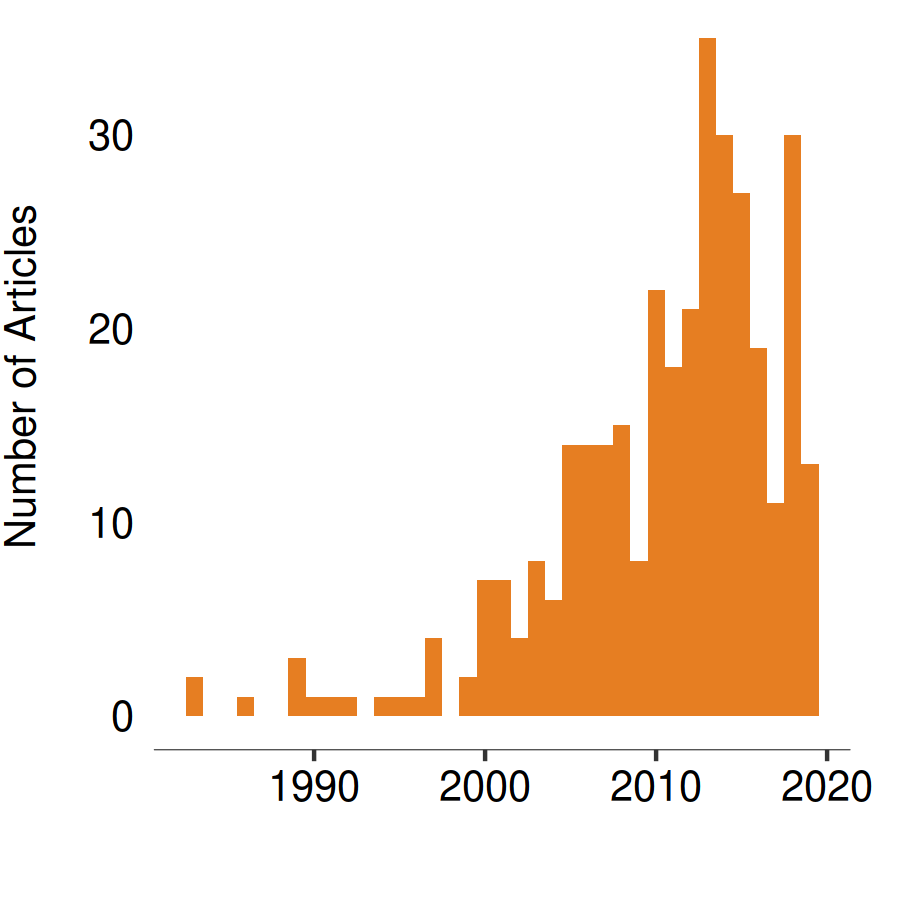
\includegraphics{images/literature-timeline.png}
  \caption{Growth of research in the area of 'Understanding distribution and dynamics of human activity' since 1980}
  \label{figure:literature:timeline}
  \vspace{1em}
  \noindent\fontsize{7}{7}\textit{Measured in the number of papers published}
\end{marginfigure}

The set of works which discuss the use of mobile devices based technologies for studying topics in disciplines such as geography \citet{li2016}, urban analysis \citep{ratti2006}, urban computing \citep{jiang2013} and other general applications and opportunities \citep{steenbruggen2013, arribas-bel2014}, serve as our starting point for this literature survey.
The search was then expanded from these reviews by navigating through their citation networks and identifying further research that are relevant.
Though this did not provide a perfectly comprehensive set of literature, it did provide a representative sample of all the different disciplines and directions of the research conducted in the area.
Through this process, around 325 relevant research publications were identified which dealt with the collection, measurement, analysis, visualisation and discussion of population and their movement at a granular level.
Research in this area started around 1950s where possibility of estimating day-time urban population at a granular level using existing  broader data employing various estimation methods were discussed \cite{foley1954, schmitt1956}.
Though this served as a starting point, the pursuit of such granular data and their applications in corresponding fields didn't pick up until the start of the 21st century during the `digital revolution' when personal computing become mainstream which was followed by the growth of internet.
Figure \ref{figure:literature:timeline} shows the yearly volume of research published since 1980 from which it can be observes that though there were some research conducted through 80s and 90s the real push forward came around beginning of the millennium when mobile phones adoption skyrocketed.
In addition to the early 2000s, a substantial increase in interest can also be seen in the beginning of the next decade fuelled by the smartphone revolution which completely changed the research avenues in-terms of volume and types of data available and methodologies available to tackle them.
While the mobile phone era put a device in every ones pockets, the smart phone era has armed them with immense data collection capabilities.
The area of research is multidisciplinary encompassing academic interest and commercial applications in various disciplines and industries spanning across wide range of themes as discussed in section \ref{section:literature:themes}.

%-------------------------------------------------------------------------------%

%==============================================================================%
% Section Introduction
%==============================================================================%

\section{Research Themes}
In this section we look at the major themes and questions tackled by this knowledge base.
We start by classifying the research into the major and minor themes explored in them as shown in Figure \ref{figure:literature:themes}.
The tree-map shows the volume of research in corresponding themes measured in terms of number of publications.
We can observe that the research is conducted in five major areas - population studies focussing on the creating and utilising data on distribution and nature of human activity, mobility and interaction focussing on the changes in these distributions, understanding the nature and function of space from these distribution and change, methods and techniques which can be used to conduct the research and finally issues and solutions related to the privacy of the users while conducting these research.
We can also observe that most of the research apart from developing methods were conducted in the domain of human mobility and social interaction closely followed by the population distribution.
In the following sections we discuss these in detail along with their sub themes with the following framework,

\begin{enumerate}
  \setlength{\itemindent}{2em}
  \itemsep-0.25em
  \item What are the major lines of questioning?
  \item What has been done previously?
  \item Where are the opportunities for further research?
\end{enumerate}

\begin{figure}
  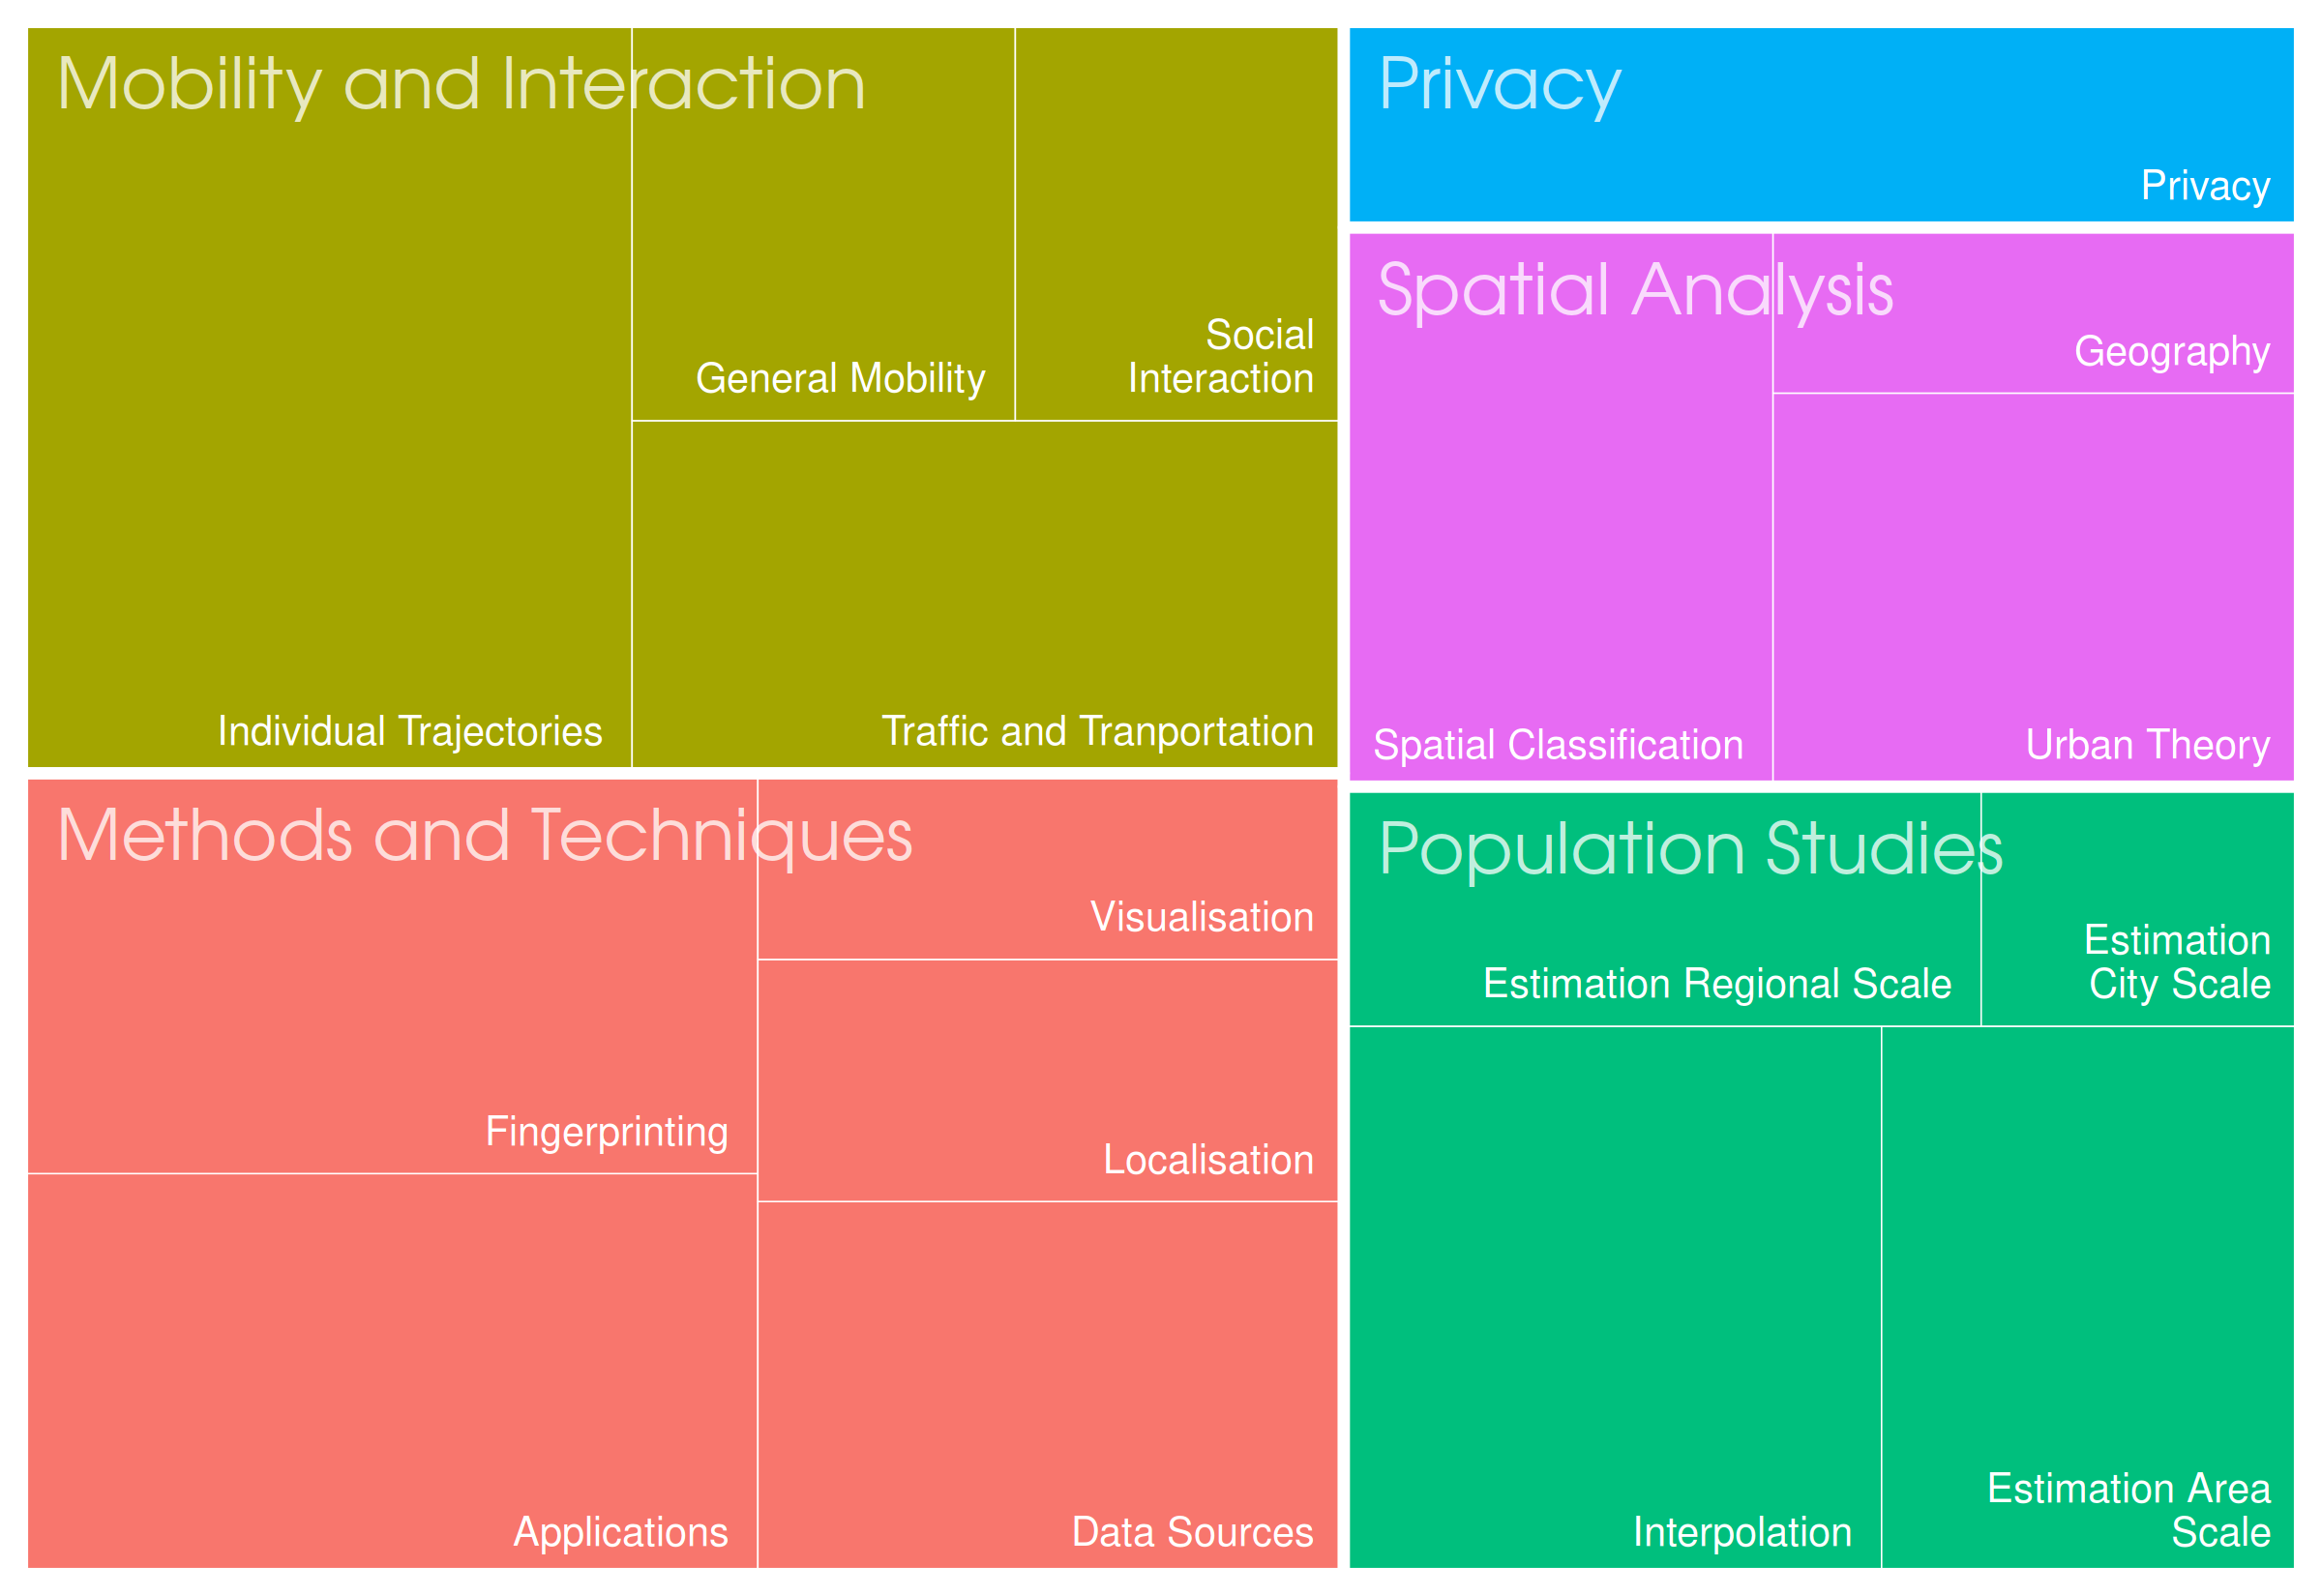
\includegraphics{images/literature-themes-treemap.png}
  \caption{Tree-map showing the volume of research conducted under each major themes and their sub-themes.}
  \label{figure:literature:themes}
\end{figure}

%------------------------------------------------------------------------------%
% Population Studies
%------------------------------------------------------------------------------%

\subsection{Population Studies}
Though \citet{foley1954} and \citet{schmitt1956} started this line of research in 1950's with the discussion on estimating daytime population using broader datasets it was not until the 80s significant volume of research kicked off in this area of study.
From 80s until mid 2000's numerous studies were conducted on measuring and studying the population at a granular level both spatially and temporally.
The focus of the research around this time was primarily on interpolation from the larger datasets created using censuses, regional or national level sample surveys and other centrally collected sources of data.
There have been numerous fairly successful attempts with methodologies where a broad dataset such  as regional level population summaries and modelling or interpolating more granular data from them by augmenting with other sources of data such as street networks \citep{reibel2005}, remote sensing \citep{sutton1997, yuan1997, chen2002} etc.
\citet{dobson2000, dobson2003a, bhaduri2002, bhaduri2007} and \citep{mennis2003, mennis2006} are examples of such research methodology.
These studies were almost done on a city scale or above with mostly modelling or interpolation methods since the data sources were few and were centrally collected.

Around 2005, there was a sharp shift in research where the interpolation methods were replaced by highly available granular data collected over cellular network.
Studies were conducted on estimating population densities, presence of tourists, general activity pattens using data from cellular networks.
Most of these research were conducted at a far larger geographic scale looking at things at an area level \citep{pulselli2008,girardin2009,phithakkitnukoon2010,yuan2016}.
There were efforts in using device level sensors such as global positioning system(GPS), Wi-Fi and Bluetooth to detect population distribution and socio-geographic routines \citep{calabrese2010,rose2010,farrahi2010}.
There have been studies on looking at people distribution as granular as queue lengths as discussed by \citep{wang2013} to city level dynamic population mapping where the limitations of traditional datasets generated through censuses and surveys \cite{deville2014}.

Around the 2015, along with the data collected directly from the mobile devices,the data that are generated by the users activity on these devices are became more important.
Social media data such as twitter \citep{lansley2016} and other consumer data such as loyalty cards \citep{lloyd2018}, smart cards \citep{ordonez2012} etc. have also become a significant sources of data for such research.
Recently, with increased concerns and legislation on privacy, there have been studies which go back to the effort of interpolating granular data from broader datasets but using more data and processor intensive technologies such as agent based modelling, deep learning, small area estimation \citep{crols2019, shibata2019, rao2015} etc..
Though there have been a lot of work done in most of the directions in this research area, the clear gap arises due to the absence of a continuous, granular and sufficiently longitudinal data-sets to complement the methodologies that have been developed. 

%------------------------------------------------------------------------------%
% Mobility and Interaction
%------------------------------------------------------------------------------%

\subsection{Human Mobility and Interaction}

This is one of the major areas of research which have significantly benefited from the decentralised collection of data at a granular level \cite{castells2000}.
In addition to being useful in their own right, these data were in turn used to augment traditional models of travel behaviour, traffic and transport to provide a better understanding of human movement over time and space \citep{janssens2013}.
The major themes of research within this area are, Movement of people in space and time with emphasis on understanding the built environment, social interaction between these people with a sociology perspective and traffic and transportation studies with a infrastructure perspective.
There is significant volume of research which dealt with recording and analysing the trajectories of the users to understand their movement patterns enabled by the unprecedented availability of detailed data from mobile devices.

% \begin{enumerate}
%   \setlength{\itemindent}{2em}
%   \itemsep-0.05em
%   \item 
%   \item 
%   \item 
% \end{enumerate}

%------------------------------------------------------------------------------%
% Methodology and Techniques
%------------------------------------------------------------------------------%

\subsection{Methodology and Techniques}

\citep{maceachren2001}
\citep{hallisey2005}
\citep{morrison2000}
\citep{lobben2003}
\citep{harrower2007}
\citep{ferrara2014}
\citep{fabrikant2005}
\citep{thomas2005}

Visualising the temporal dynamics of data collected on human activities through decentralised processes poses significant challenges when approached with traditional cartographic concepts (MacEachren, 2001 Hallisey, 2005).
Digital media especially animation has been explored as an option to solve for the temporal dimension (Morrison, 2000; Lobben, 2003) but is bound by the cognitive limits of the viewer (Harrower, 2007).
There have been approaches proposed around animations of generated surfaces (Kobayashi, 2011) and network-based visualizations (Ferrara, 2014) leaving gaps in research for new methods in dynamic geographic visualisation (Fabrikant, 2005) and visualising path and flow of phenomena (Thomas, 2005).
This provides us with a promising opportunity for research in methods for visualising high frequency, hyper-local pedestrian data within the limits of cognition of the viewer.

%------------------------------------------------------------------------------%
% Spatial Analysis Theory and Modelling
%------------------------------------------------------------------------------%
\subsection{Spatial Analysis - Theory and Modelling}

Traditional and modern geography was dominated by the study of centrally collected data acquired through extensive field surveys and remote sensing.
In the last two decades, a significant paradigm change has been introduced by the availability of unprecedented amount of data generated by unconventional sources such as mobile phones, social media posts etc.
This move to the postmodern geography has been accompanied by a change in our understanding of the built environment and human geography from a static point of view to a more dynamic definition \cite{soja1989}.
This definition is based on the bottom-up mechanisms which make human activity such as information exchange and economy to manifest in the physical built environments as argued by \citep{batty1990, batty1997, batty2012} and \citep{batty2013, batty2013a}.

This transition into the digital age \citep{graham1999, tranos2012, tranos2013} has changed the politics of space and time \citep{massey1992} and been more pronounced in the study of urban built environment where technology has redefined the concepts of place and space \citep{graham2001, graham2002, sassen2001}.
With the ability to collect and analyse of data on large complex systems in real-time \citep{graham1997}, we are exploring the possibilities of understanding their structure and organisation using concepts of complexity theory \citep{bettencourt2013, portugali2012} with more emphasis on their temporal patterns such as the argument towards finding the pulse of the city \citep{batty2010}.
With the population getting more and more connected \citep{castells2010}, the nature of space/place is being dynamically defined by the population themselves \citep{giuliano1991} and vice versa \citep{zandvliet2006}.
This flood of hard data \cite{nature2008} was accompanied not only by optimism in its potential \citep{thomas2001} but also by the questions raised on the challenges in handling the diverse, large scale, non standardised data it produces and the usefulness or representativeness of the resulting analysis \citep{miller2010, arribas-bel2014a}.

However, availability of such data has impressive uses in urban studies \citep{bettencourt2014} especially with advancement of new technologies \citep{steenbruggen2015} and possibility of distributed, crowdsourced data collection \citep{lokanathan2015}.

%------------------------------------------------------------------------------%
% Privacy
%------------------------------------------------------------------------------%
\subsection{Privacy}

The ubiquity of personal devices and digitisation of day to day activities through these mobile devices \citep{mcmeel2018dark} has provided many opportunities for researchers and industry for collecting, analysing and deriving inputs from them.
However at the same this also increased the risk of infringement on privacy of the users whose data is being collected \cite{saponas2007, krumm2009}.
There is immense value in uniquely identifying and profiling information on people for specialised purposes such as security \citep{cutter2006} and law enforcement \citep{dobson2003} but also has extreme risks associated when not handled with care \citep{vanwey2005}.

Strictly protecting personal information while ensuring the information is usable for research by maintaining the uniqueness in the data is the major concern which was addressed by devising frameworks for secure practices in confidentially collecting and using the location data \citep{duckham2006, tang2006, lane2014}.
Some efforts sought to accomplish this task through cryptographic hashing algorithms (Pang, 2007) while others aimed to thwart identification and tracking at the device level by techniques such as MAC randomisation \citep{gruteser2005, green2008}.
Finally though getting consent of users for the collection and use of such information from their mobile devices is challenging, there is a significantly improved acceptance when the process offers value in return such as discounts and monetary benefits \citep{kobsa2014user}.

There is opportunity in this area for research in applying the cryptographic solutions along with the privacy preserving frameworks to arrive at methods which can extract useful information out of large personal data while obscuring or anonymising them.

%==============================================================================%
% Research Trends
%==============================================================================%

\begin{figure*}
  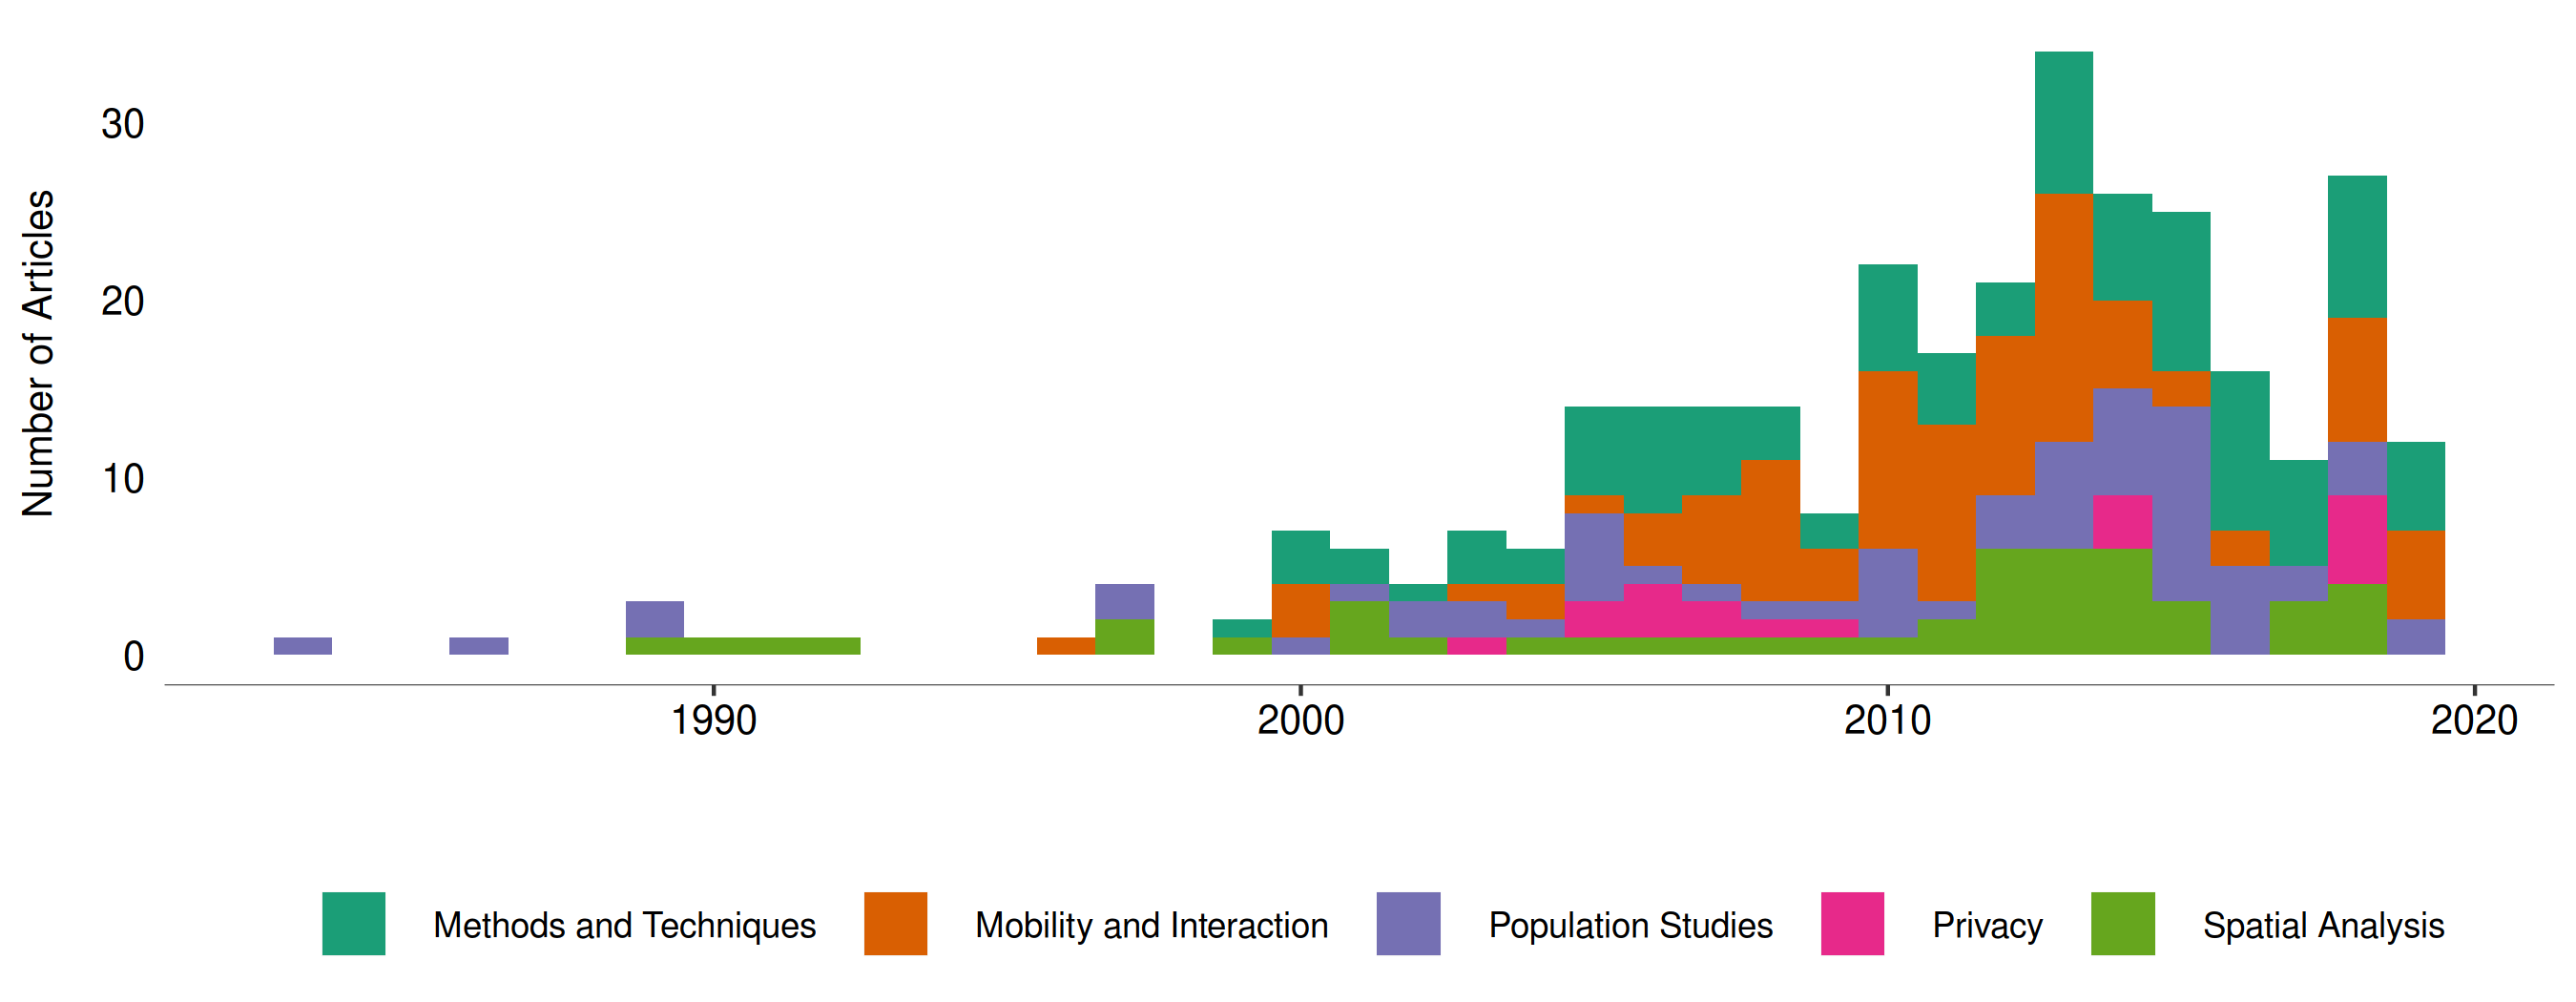
\includegraphics{images/literature-themes-timeline.png}
  \caption{Outline of the `Medium data toolkit' devised to collect, process, visualise and manage the Wi-Fi probe requests data}
  \label{figure:literature:themes:timeline}
\end{figure*}

\section{Research Trends}

Figure \ref{figure:literature:themes:timeline} shows the volume of research done in this topic since 1980 categorised based on their major themes discussed earlier.
We can observe that there are distinct trends in the research over time, which evolved around the development of technology in the last two decades.
Until 90s the research was mostly centered around population studies on estimating and interpolating granular spatial and temporal information from larger and cross sectional datasets such as census and sample surveys.
The period between 2000-2010 there was interest in potential of the new data generated by the digital revolution. 
We can categorise this as the `mobile era' where carrying mobile devices become mainstream.
This explosion of research coincided with mobile phones becoming more popular and ubiquitous with population in urban areas and was around development of methods and techniques to utilise the data generated from them.
There were also extensive studies in using the datasets to understand human mobility along with a rising concern in the privacy of the users who's data which are being used for these studies.

%------------------------------------------------------------------------------%

The release of iPhone in 2008 and the increase in the share of 'smartphones' in the next 10 years sparked the `smartphone' era. 
The change made sure that all the mobile devices gaining numerous capabilities such as internet connectivity over Wi-Fi and mobile network, location awareness with global positioning system, movement recognition with accelerometers and connectivity other `wearable' devices through Bluetooth.
This also lead to the digitisation of lifestyle where every aspect of the life being done through these devices over internet while generating huge amount of data on these activities.
This sparked the large volume of research on the form and function of space by studying this data and on the dynamics of human population in space and time in the next 5 years.
These research were particularly centered around tracking the trajectory of people using the mobile devices they carry with them as the smartphones made it easier to collect the necessary data directly from them rather than depending on a centrally collected datasets from mobile carriers. 
With the theoretical limit to predictability in human mobility quantified \cite{song2010limits}, the focus on urban mobility has been declining in the past few years which has led to a renewed interest in population studies at a local-local level in real-time.
In addition to using the data from the mobile devices, these studies have also been exploring the use of large assemblages of consumer data that are being generated in this connected mobile environment and linking them together to create a fuller picture \cite{cdrc2018}

%------------------------------------------------------------------------------%

Finally, with the increase in use of personal data, there has also been an increase in research regarding the privacy of the users.
Along with this, the mobile devices and subsequently the data generated by them are more and more anonymised so that the users cannot be tracked or identified at a personal level.
This has given rise to the new trend in research to devise methods to overcome this anonymisation and at the same time research which considers these methods as vulnerabilities and find solutions to make the anonymisation process more robust. 
There is clear need for methods which anonymise the data sufficiently to protect the identity of the users and at the same time enable us to conduct research in
measuring studying population distribution and movement at a granular level.

%==============================================================================%
 

%------------------------------------------------------------------------------%
\section{Techniques and technology}\label{section:literature:technology}
%------------------------------------------------------------------------------%

\begin{marginfigure}
  \forcerectofloat
  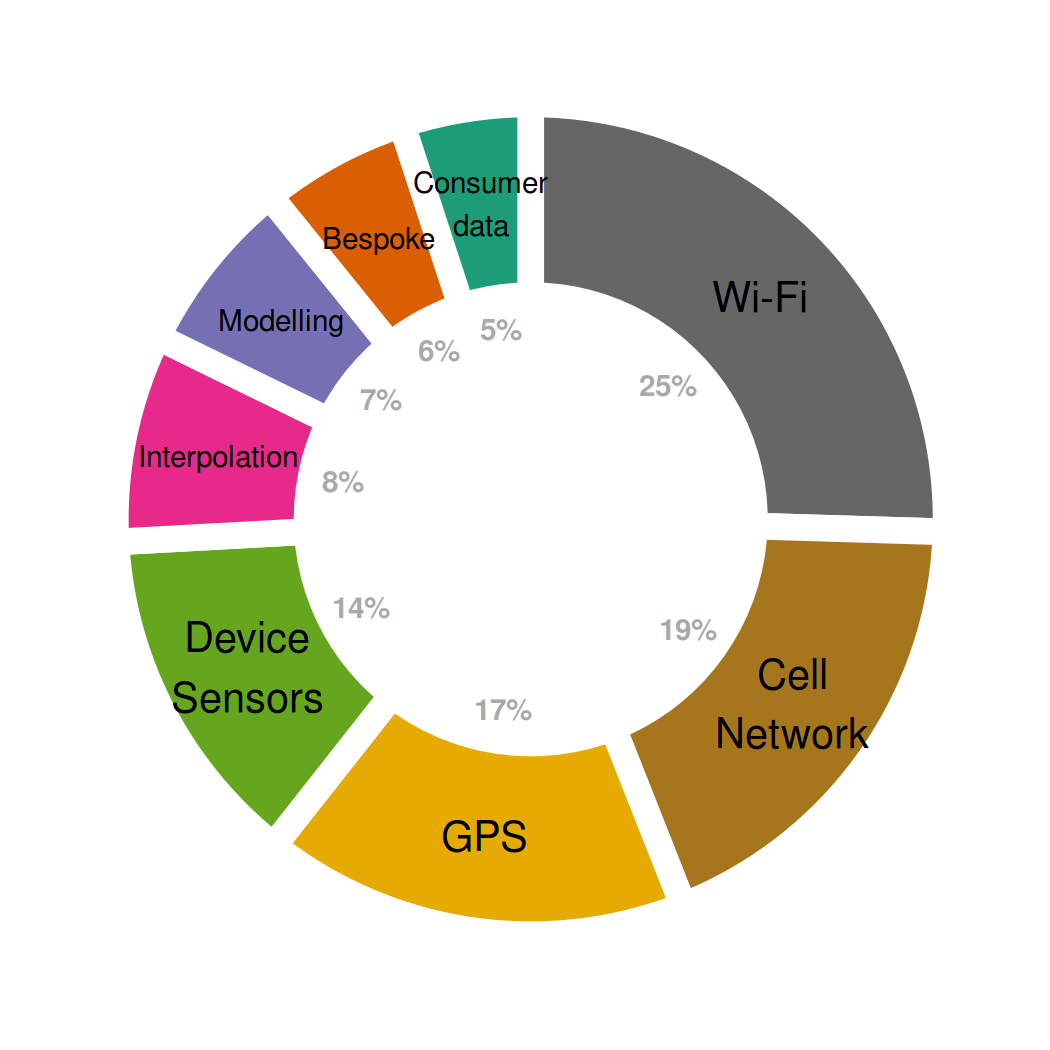
\includegraphics[trim={1.1cm 1cm 1cm 1cm},clip]{images/literature-technology.png}
  \caption{Distribution of research across various techniques and technologies}
  \label{figure:literature:timeline}
\end{marginfigure}
\marginnote{\noindent\fontsize{7}{7}\textit{Measured in the number of papers published}}

When we look at the literature from the technology perspective, we observe that over the years, the research continuously picks up and applies recent technological developments in the pursuit of understanding the distribution of human activity and population.
Figure \ref{figure:literature:timeline} shows the distribution of the research in terms of the main technique/ technology used over the past 40 years.
We observe that the earliest attempts started from the exploration of using interpolation and modelling techniques on a broader dataset.
As the need for more granular datasets increased there were attempts to devise and utilize bespoke solutions to generate them.
When mobile devices became mainstream, the focus shifted to utilize the relevant components of the mobile infrastructure.
A significant number of studies were done in utilising data collected from the mobile network, sensors in the mobile devices, especially GPS and Wi-Fi, in addition to the social media content generated from these devices.
A detailed account of these studies is given below,

\begin{figure*}
  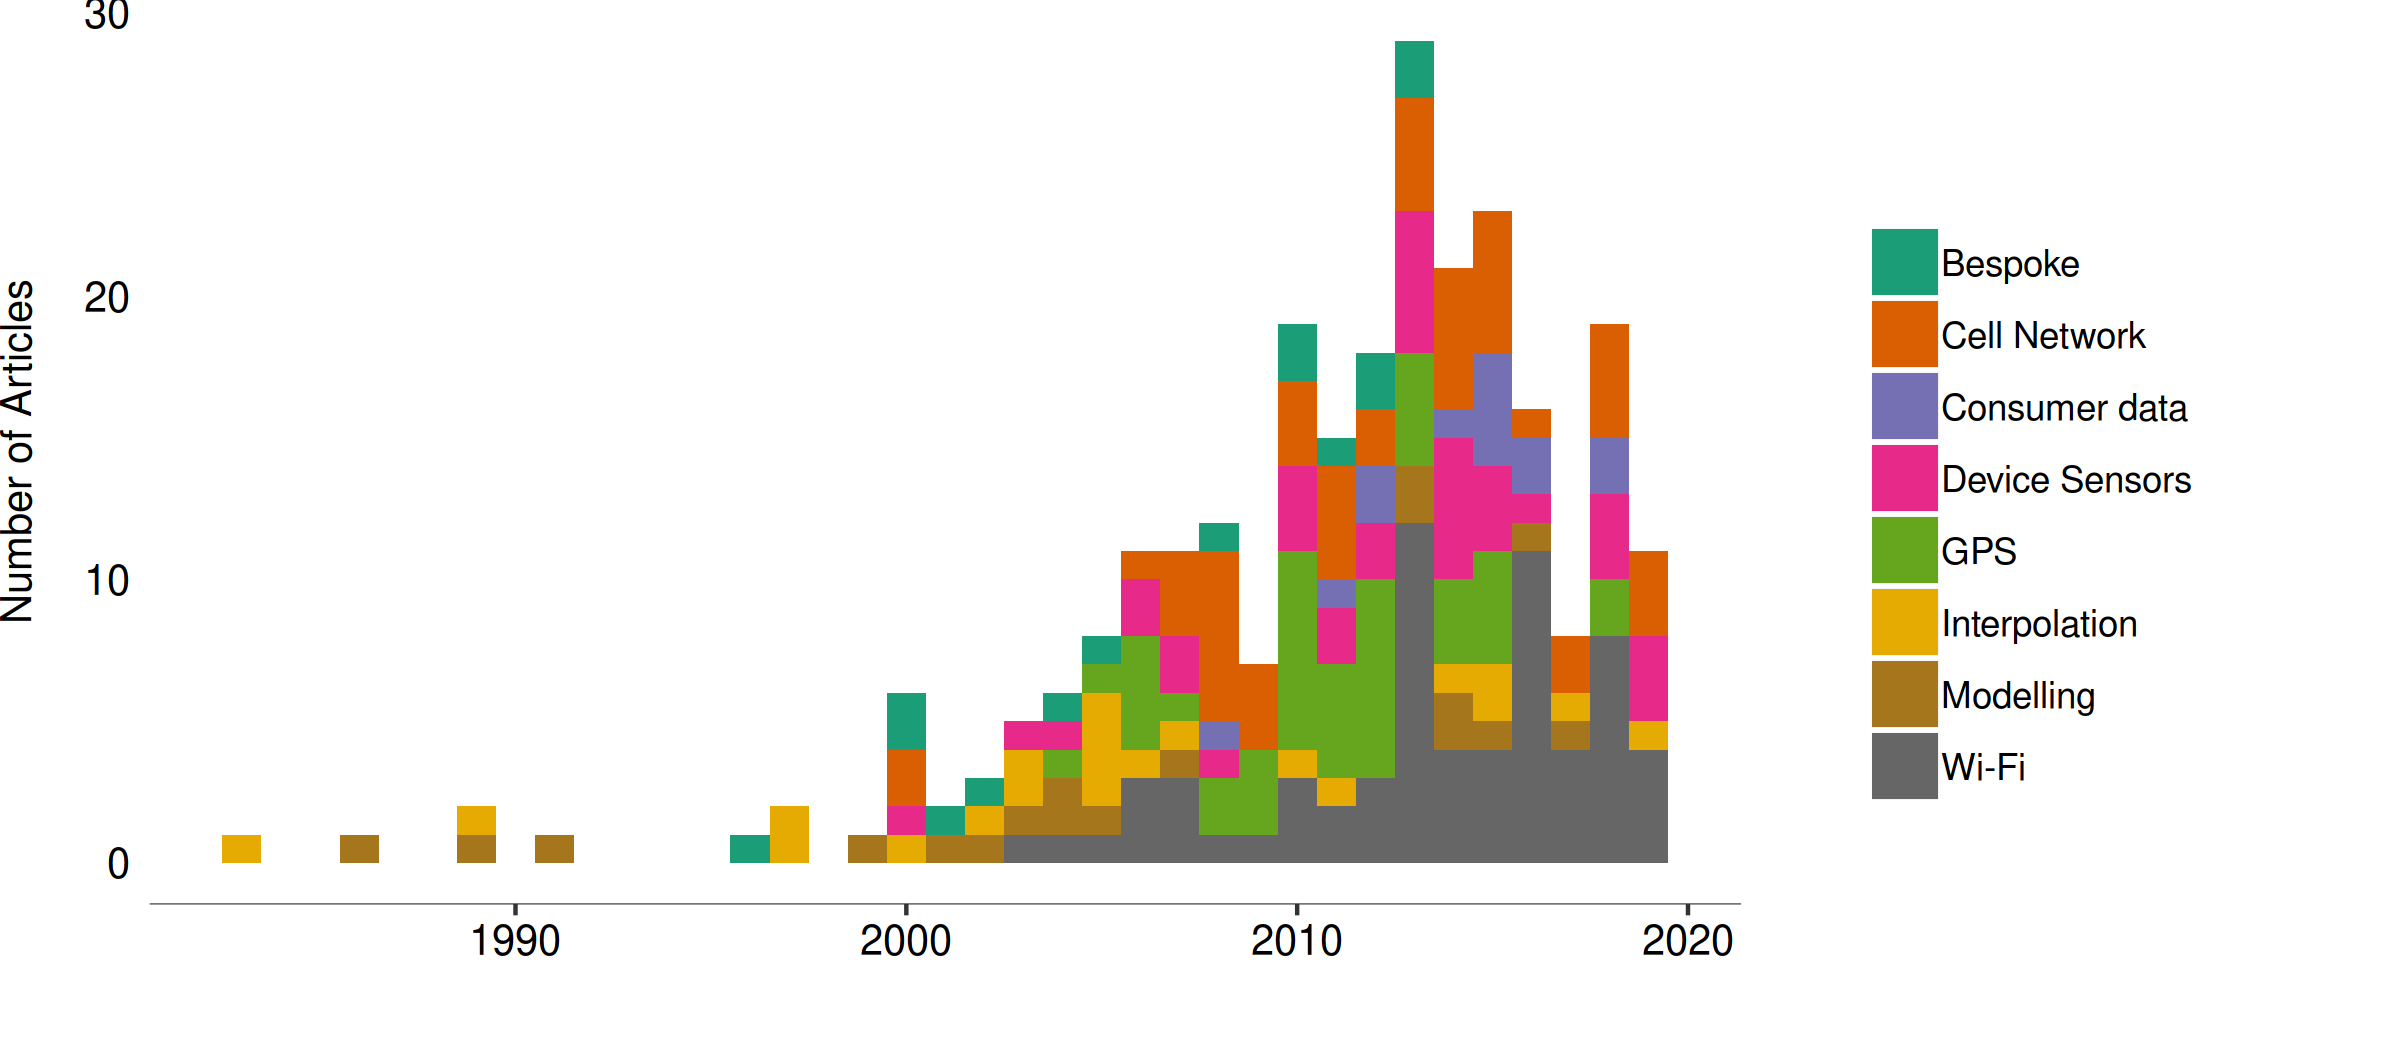
\includegraphics{images/literature-tech-timeline.png}
  \caption{The evolution of research since 1980 in terms of the the technology used in the research.}
  \label{figure:literature:tech:timeline}
\end{figure*}

%------------------------------------------------------------------------------%
\subsection{Interpolation and Modelling}
%------------------------------------------------------------------------------%

Attempts in using the existing data collected through traditional methods such as census and large scale sample surveys to create spatially and temporally granular and detailed estimates were carried out by applying various interpolation methods such as pycnophylactic, dasymetric interpolation \citep{tobler1979, mennis2003, mennis2006, hawley2005, tapp2010, wismans2017} along with spatial \citep{lam1983,martin1989, martin2015} and temporal interpolation techniques \citep{glickman1986}.
These methods along with supplementary data such as remote sensing imagery \citep{sutton2001, chen2002} and street networks \citep{reibel2005} were shown to be useful in producing detailed granular population maps at various scales with varying degree of success \citep{dobson2000, bhaduri2002, dobson2003, bhaduri2005, bhaduri2007}.
These approaches have been employed in various applications such as econometric studies \citep{mcdonald1989}, studies on public health \citep{hay2005}, emergency management \citep{kwan2005} and flood risk estimations \citep{smith2016}.

In addition to these interpolation techniques classic modelling techniques can also be used to estimate daytime populations and demographic structure at hyper-local scales \citep{jochem2013, jia2014}, urban scales \citep{alahmadi2013, abowd2004} and regional scales \citep{foley1954, schmitt1956, singleton2015, mccormack2017}.
The granular data created with such modelling techniques are shown to be useful in urban planning and management \citep{parrott1999}, emergency management \citep{alexander2002, cutter2006} and in modelling traffic and transportation \citep{lefebvre2013}.
These interpolation and modelling techniques along with granular data produced are also used in classifying spatial areas and hence understanding the structure of cities in general \citep{mcmillen2001, mcmillen2004, lee2007, arribas-bel2014}.
Though being useful, these techniques are still shown to have limitations and uncertainties \citep{nagle2014}, which mostly arise from the nature of the input data employed.
This leads us to the need for more detailed and frequent collection of data.

%------------------------------------------------------------------------------%
\subsection{Bespoke technologies}
%------------------------------------------------------------------------------%

Following this need, there has been efforts to use bespoke or specialised technologies such as cameras \citep{cai1996, heikkila2004, krockel2012}, Lasers \citep{zhao2005, arras2008} and radio frequency receivers  \citep{bahl2000, yang2013, chothia2010, bulusu2000, dil2011} to measure human activity.
But the major problem with such solutions is the cost and effort involved in designing and implementing them at urban and regional scales comprehensively.
Moreover, being specialised and centralised they tend to be challenging to maintain and update as the technological landscape change.
This gives us the need to identify and use techniques which are more general in nature and can be used for longer periods of time which are cheap to install to achieve a more comprehensive coverage.

%------------------------------------------------------------------------------%
\subsection{Cellular Network}
%------------------------------------------------------------------------------%

The rise of mobile phones as ubiquitous personal devices for the broader population has provided us with a viable alternative for collecting data with finer granularity at large scales.
Mobile infrastructure consists of both the `network part’, built and managed by the service providers, and the `user part’, which is the phones owned by the users’ themselves.
The network part, in addition to providing connectivity to the users, also collects information on these devices actively such as communication between the users and passively such as when the phones themselves move from tower to tower.
The mobile devices themselves have a variety of sensors such as accelerometer to identify movement, compass to identify orientation, GPS receiver to deduct geographic position, etc.
They also have various communication capabilities such as cellular, Wi-Fi, Bluetooth and Near field communications (NFC) etc. 
Both of these sensors and communication capabilities can be used as sources of data themselves.
With the growth of mobile devices and the infrastructure surrounding it, there has been significant effort in utilising data generated by every component of this complex infrastructure.

The first set of research started to use the cellular network data for urban studies \citep{jiang2013,steenbruggen2015, lokanathan2015, calabrese2015, reades2007}.
Even though this approach has been acknowledged to have inherent biases such as ownership bias across particular demographic groups \citep{wesolowski2013} the relative advantages such as coverage made them excellent sources of data.
Visual exploration of use of such data using interactive interfaces to evaluate quality of service and scenario testing has been tested for the optimisation of public transport \cite[-4cm]{sbodio2014}.
Such network data with the active and passive information collected from them can be used to create trajectories of people \cite{schlaich2010}, detect their daily routine \cite[2cm]{sevtsuk2010} and classify those routes in terms of function \citep{becker2011a}.
It was also demonstrated to be useful in understanding overall mobility and flow of people and information \citep{candia2008, krings2009, simini2012, zhang2019}.
These data can be used to identify asymmetry in flow of people spatially \citep{phithakkitnukoon2011}, estimate volume and pattern of road usage \citep{bolla2000, wang2012} and by augmenting the topology to optimise operations \citep{puzis2013}.
Such datasets have been extensively used in traffic and transportation research to derive origin-destination matrices \citep{caceres2007, mellegard2011, iqbal2014}, travel time estimation \citep{janecek2012} and traffic status estimation \citep{demissie2013, grauwin2015}. 

It has been shown that mobile network data can be used to uncover nature of the population such as tourists in specific areas \citep{girardin2008} and the interaction between the people in the study area \citep{campbell2008}.
The structure \citep{onnela2007, onnela2007a}, geography \citep{lambiotte2008} and dynamics \citep{hidalgo2008} of such networks have been studied and demonstrated to be useful in predicting their change \citep{wang2011, vajakas2018} over time.
This social networks and their spatio-temporal structure can also be used for classification of land use \citep{pei2014, jia2018}, assessment of spatial patterns \citep{reades2009, steenbruggen2013} and understanding the broader spatial structure of cities \citep{louail2014, arribas-bel2015} and regions \citep{arhipova2018}.
The data collected from the cellular network when examined at granular levels such as inter-personal communication and economic activity can be used to create estimations of micro area-level population density \cite[-4cm]{pulselli2008, ng2017} and also the characteristics \cite[1cm]{girardin2009} and the nature of the activity \citep{phithakkitnukoon2010}.
Aggregated human activity measured from such research in turn can be used to measure and model population dynamics and land use density and mix at broader level \citep{jacobs-crisioni2014, tranos2015, tranos2018}.
The spatial patterns thus uncovered can then be applied to urban planning \citep{becker2011b} whilst the temporal patterns uncovered have immense utility for the disciplines such as epidemiology.
For example, population influxes measured from changes in mobile network usage can be used to model spread of diseases \cite{buckee2015}.

Though the mobile network provides much more granular and accurate data than interpolation techniques, it is not without its limitations \citep{yucel2017}.
The distribution of network infrastructure usually follows the purposes of service coverage and follows commercial decisions. 
This introduces systematic biases in the data passively collected through them.
Moreover, the data actively collected through them has bias based on the volume of usage of services by the customers which can vary widely spatially, temporally and also based on demography.
In addition to this because of the coverage, the data collected from mobile service providers pose immense privacy risk when linked to other sources of consumer data.
This makes collection of data directly from the devices using the sensors on the device much more robust in certain cases.

%------------------------------------------------------------------------------%
\subsection{Mobile Sensors}
%------------------------------------------------------------------------------%

The most prominent sensors and capabilities present in mobile devices that can be used for distributed urban sensing are Cellular radio, Bluetooth, Wi-Fi, GPS, accelerometer and compass \cite[-5cm]{lane2010, zhu2018}.
Since cellular radio is managed by the cellular network and covered in mobile network data, we explore the research done with other sensors.
In contrast to planned actively collected data, data passively collected via a distributed network of general purpose devices tends to be larger and more temporally dynamic.
For example, an organised survey conducted every month to understand interpersonal communications between people in a team of 50 will result in a 2500 records a month.
The same task is done through collecting data on email communication sent by them will result in a same volume records in a day.
The challenges and solutions on collecting and analysing such large-scale longitudinal data are discussed by \citep{laurila2012, antonic2013}.
The real time nature of such data also gives us the opportunity to monitor and understand the city in much smaller temporal scales \citep{townsend2000, oneill2006} and the representativeness of such datasets have also been explored \citep{shin2013, kobus2013}.
Data generated from communication networks can be used to understand the structure of urban systems which are becoming increasingly border-less \cite{bertolini2003}.
Similar to the network based data, it can help in understanding human mobility \citep{asgari2013, amini2014, zhang2014} through mining trajectory patterns \citep{giannotti2007} and socio geographic routines \citep{farrahi2010}.
It is also useful in various traffic and transportation applications for monitoring roads \citep{mohan2008} and estimating traffic \citep{cheng2006}, uncovering regional characteristics \citep{chi2014} and extracting land use patterns \citep{shimosaka2014}.
Apart from GPS and Wi-Fi, there have been efforts in exploring other possibilities such as Bluetooth for location \citep{bandara2004, becker2019} and aggregate detected Bluetooth activity to monitor freeway status \citep{haghani2010}.
There have also been successful implementations of frameworks to predict movement of people by combining Wi-Fi and Bluetooth \cite{vu2011}.
But owing to shorter range and requirement of active engagement from the user where they have to actively start the device pairing process, Bluetooth is much less preferable for large-scale data collection than GPS or Wi-Fi.
The research on GPS and Wi-Fi based studies are discussed in more detail below.

%------------------------------------------------------------------------------%
\subsection{Global Positioning System}
%------------------------------------------------------------------------------%

In addition to providing a user’s location to applications such as maps and navigation, the GPS capability in mobile devices in tandem with Wi-Fi can also maintain a continuous list of locations visited by the device over long periods of time.
It works mostly in the background and requires almost no active input from the user to operate.
Though very convenient for collecting data, due to the privacy risks associated with it, GPS is often one of the resources in a device that requires explicit user permission to be accessed.
The concepts and methodologies for collecting such data were set out by \citep{asakura2004} and there have been attempts to collect this rich data from volunteers at a large scale along with ancillary data \citep{kiukkonen2010} and provide a location based service application for the collection of data \citep{ratti2006, jiang2006, ahas2005}.
 
The accuracy, convenience and being designed for navigation makes GPS one of the most used technologies for mobility studies \cite{gonzalez2008}.
It has been used to analyse and understand individual mobility patterns \citep{neuhaus2009, shin2010}, which have been shown to have a high order of regularity in spite of the complexity \citep{brockmann2006, song2010a}.
There have been efforts to use this regularity to predict the future location of people \citep{monreale2009, calabrese2010}.
The limitations of predictions have also been quantified \citep{song2010}.
There have been successful efforts in extracting behaviours and patterns from such trajectory data \citep{liu2010, cho2011, hoteit2013, pappalardo2013} along to understand individual patterns from large assemblages \citep{giannotti2011, calabrese2013} and vice versa \citep{wirz2012}.
In traffic and transportation, GPS trajectory from mobile devices is used to estimate \citep{calabrese2011} and expand \citep{jing2011} origin-destination matrices, detect the mode of travel \citep{gong2012, rossi2015} and calibrate existing spatial interaction models \citep{yue2012}
.
Since the data is collected at the device level and depends on the activity of the individual, it can be de-anonymised to reveal the nature of the owner of the devices.
The possibilities of detecting the activity of the individual from trajectory information is demonstrated by \citep{liao2006, krumm2007}.
Patterns \citep{jiang2012} and structures in routines \citep{eagle2009} can be extracted from these trajectories and can be used for socio geographic analysis of the population \citep{licoppe2008, chen2018}.
It can also utilised in classification of the population at a particular location at a given time \cite[-1cm]{pappalardo2015}.
Being inherently spatial and activity driven, GPS trajectories have been shown to be useful to identify \citep{bao2012}, characterise \citep{wan2013} and automatically label \citep{do2014} significant places of interest.
It can also be used for land use detection \citep{toole2012, zhang2018}, classification \citep{jiang2015} and the study of urban morphology \citep{kang2012}.
These GPS trajectories have been shown to be useful in estimating population dynamics at local level and within short durations during social events \citep{calabrese2010, kim2014, deville2014}.
When combined with other data sources can be useful to understand relationship between spatial areas \citep{long2015}.

From the literature we see that GPS is one of the most precise and accurate user side methods of collecting location of mobile devices.
In addition, the data collected is well understood and collection methodologies can be scaled up with minimum resources.
That being said, it is also well established that urban sensing methods using GPS of mobile devices has problems of enhanced risk of breach of privacy when executed passively and need explicit user engagement when executed actively.

%------------------------------------------------------------------------------%
\subsection{Wi-Fi}
%------------------------------------------------------------------------------%

Wi-Fi is a wireless network connection protocol standardised by \citet{ieee2016}.
It is a distributed server-client based system where the client connects to access points (AP).
Every mobile device in the network has a unique hardware specific MAC address, which is transmitted between the device and AP before the connection is made.
The key feature of Wi-Fi infrastructure is that the network is distributed and the APs can be set up and operated by anyone locally unlike mobile networks.
Since they are primarily used for Internet service provision, the protocol has priority for continuity of connectivity so the devices constantly scan for new and better connections.
This is done through a probe request, which is detailed in later sections.
With this background we can see that Wi-Fi provides a fair middle ground between an entirely network driven approach such as cellular network to an entirely user driven approach such as GPS.
Since the network infrastructure is distributed and deployed for Internet it offers more coverage than most of the technologies discussed except or cellular network. It is also very resilient and can encapsulate and reinforce civic space in cities \cite[-2cm]{torrens2008}.

Though Wi-Fi is a location less technology, there are reliable methods to trilaterate the location of the device by the signal strength and the locations of APs known through either targeted surveys or crowdsourced volunteer effort \citep{he2003, moore2004, lamarca2005, dinesh2017, lin2018}.
This can overcome the usual shortcoming of GPS, which struggles for precision and accuracy in indoor and densely built environments \citep{zarim2006, kawaguchi2009, xi2010}.
Utilising this, we can easily and quickly estimate trajectories of the mobile devices just using the Wi-Fi communication the device has with multiple known APs \cite[-4cm]{xu2013}.
This can be used similar to the GPS trajectories to understand individual travel patterns \citep{kim2006, rekimoto2007, sap2015}, crowd behaviour \citep{abedi2013, mowafi2013, shu2017}, vehicular \citep{lu2010} and pedestrian movement \citep{xu2013, fukuzaki2014, wang2016, taylor2019}.
It can also be used in transportation planning and management to estimate travel time \citep{musa2011, haakegaard2018} and real time traffic monitoring \citep{abbott-jard2013}.

Being a general network protocol designed to be used by mobile devices, Wi-Fi devices relay a range of public signals known as probe request frames on regular intervals throughout its operation, for the purpose of connecting and maintaining a reliable and secure connection for the mobile device \cite{freud2015}.
These signals can be captured using inexpensive customised hardware, non-intrusively and in turn to be used for numerous applications.
In addition to a uniquely identifiable MAC address, these signals include a range of other information which when combined with the temporal signatures of the signals received can help us understand the nature and identify the devices which are generating these signals.
These device/user fingerprinting techniques are demonstrated by \citep{franklin2006} and \citep{pang2007} and the unique MAC addresses and associated information can successfully track people across access points \cite{cunche2014a}, their trajectories \citep{musa2012}, the relationship between them \citep{cheng2012, barbera2013, cunche2014} and predict which of them will be most likely to meet again \citep{cunche2012}.
Using the semantic information present in these probe requests, such as names of previously connected APs, it is possible to understand the nature of these users at a large scale \citep{di2016}.
Using the received signal strengths from pre placed devices we can monitor the presence and movement of entities that are not even carrying a Wi-Fi enabled device \cite{elgohary2013}.

Because of the security and privacy risks posed by the Wi-Fi protocol’s use of hardware based MAC address, various methods to strengthen the security have been proposed \citep{pang2007, greenstein2008}.
The randomisation of MAC addresses has become more mainstream in mobile devices with the introduction of it as a default operating system behaviour in iOS 8 by Apple Inc.
Since MAC randomisation is not a perfect solution \citep{mathieucunche2016} there have been numerous attempts to fingerprint unique devices from the randomised anonymous information present in the probe request frames for the purposes of trajectory tracking and access point security.
The methods used are decomposition of OUIs where detailed device model information is estimated by analysing an already known dataset of OUIs \cite{martin2016}; Scrambler attack where a small part of the physical layer specification for Wi-Fi is used \citep{bloessl2015}; and finally, the timing attack where the packet sequence information present in the probe request frame is used \citep{matte2016, cheng2016}.
A combination of these methodologies has been proven to de-anonymise randomised MAC addresses \citep{vanhoef2016}.
In addition to tracking, Wi-Fi probe requests can be aggregated to uncover the urban wireless landscape \citep{rose2010} and used to reveal human activity at large scales \citep{qin2013}, pedestrian numbers in crowds \citep{schauer2014, fukuzaki2015} and also counting people in hyper local scales such as queues \citep{wang2013}.
With enough infrastructure we can aim to generate a real-time census of the city \citep{kontokosta2016} and also predict the amount of time a device will spend around the sensor as well \citep{manweiler2013}.
Similar to GPS data this can be used as an additional control layer for interpolation techniques such as map merging \citep{erinc2013}.

\citep{pinelli2015} looks at a comparison of various approaches of collecting and analysing mobile phone location data.
The research identifies two major approaches in collecting device location data - Event-driven and Network-driven.
The event-driven approach is centered around the mobile devices generating data 
through their day to day activities.
The major sources of event-driven data are Call Detail Records(CDR) and internet use.
Network-driven approach is centered around the service provision infrastructure such as cellphone towers, Wi-Fi base stations etc.
The methods used to collect network-driven data are periodic update - where the device sends an update stating the base station it is connected to, handover - where the device information is recorded as they are moving between base stations and location update - where the location of the device is recorded based on the base stations it is connected to. 
The research used a set of anonymised mobile phone location data from a Belgian telecom operator for the city of Mons from which various event-driven and network driven scenarios were simulated. 
The authors compared the advantages of these simulated scenarios for application-independent and application-dependent cases such as spatial dispersal, classes of users, count estimation and flow estimation.
Through these comparisons it was shown that using network-driven mobile phone location data is more advantageous compared to the widely used event-driven ones.

%------------------------------------------------------------------------------%
\subsection{Consumer data}
%------------------------------------------------------------------------------%

In addition to the direct data from the sensors themselves the content generated from the mobile devices such as social media data or smart-cards \cite{zhong2016} can provide a viable proxy for estimating the level and nature of human activity.
The use of geo-located tweets on the study of small-area dynamic population estimation \citep{ordonez2012, marchetti2015, mckenzie2015, lansley2016a}, geo-demographics \citep{bawa-cavia2011, longley2015, lansley2016b} and global mobility \citep{hawelka2014} has been thoroughly explored.
These data sources are shown to be useful in social sciences \citep{crane2008}, abnormal event detection \citep{chae2012} and analysing urban environments \citep{sagl2012}.
It can also be used as a control layer for interpolation techniques we discussed earlier \citep{lin2015}.


\section{Discussion and Research Gaps}

From the above literature search we can conclude there is a considerable opportunity in the application of mobile phone based data to be used to measure small-scale spatio-temporal dynamics of human activity and potential for research gaps in the following areas:
Hyper-local population estimation This research is at the limits of acceptable mobility research in the context of privacy concerns i.
 between the explosion of usage of smartphones and implementation of MAC randomisation.
The availability of identifiable device information has led to a considerable effort in urban mobility studies and there are still opportunities in real time small-scale population measurement and estimation.
Detailed WiFi data, combined with other data sources such as public transport, weather etc.
along with interpolation and modelling techniques can produce detailed spatio-temporal estimates of population at local level.
De-Anonymisation of devices The increase in privacy concerns and the normalisation of device level security measures such as MAC address randomisation has questioned the basic assumptions about the reliability of data collected through mobile devices.
There is a definite research need and interest in finding a method to uniquely identify devices with sufficient confidence while not deciphering any personal data from such analysis.
Device classification There has been a significant volume of studies in the classification of space based on the temporal patterns in the human activity around them and classification of human activity based on the space it is clustered around.
But there is a research opportunity in looking at these devices closely, especially their temporal patterns around the point of interest to make inferences about the nature of the device.
This idea is closely related to de-anonymisation discussed about but rather than trying to find unique users or devices from a set of signals, we try to find the groups of similar devices and connecting these groups to meaningful typologies.

Sensor catchment and flow Having access to a broader sensor data, we can cross-sectionally see the distribution or occurrence of a unique MAC address / device and determine the influence of a sensor.
This can be approached in two ways: the first being the pedestrian flow approach where we can model the movement of pedestrian based on these relationships and the second is treating these relationships as network and detecting communities in them.
In addition to these, there is a definite opportunity for research in methods for visualising high frequency, hyper-local pedestrian data within the limits of cognition of the viewer.

In terms of technology, which can be used for data collection at local level, the summary of the advantages of each is given below,

	Interpolation
	Bespoke Systems
	Cellular Network
	GPS 
	WiFi
	Coverage
	-
	Local
	City to National
	Local to Global
	Local
	Certainty
	Very Low
	High
	Medium
	High
	Medium
	Independence*
	Low
	Very High
	Low
	Medium
	High
	Intrusiveness
	Low
	Medium
	High
	High
	Medium
	Granularity
	Very Low
	Very High
	Medium
	High
	High
	Ease of Collection
	Medium
	Low
	Medium
	Low
	High
	Scalability
	Medium
	Low
	High
	Medium
	High
	Privacy Risk
	Low
	Medium
	High
	High
	Medium
	

Table 2.
: Evaluation of advantages of different approaches that can be used for data collection.
*independence from secondary data collected by a third party.
From Table 2.1 we can see that though it poses some risk on privacy of participants and some uncertainty regarding range, WiFi offers the best possible technology for data collection through mobile devices at smaller scales.


\cleardoublepage
\chapter{Collecting the Data}

As we saw in the literature search Wi-Fi as a technology is well suited for research into human mobility.
In this chapter we evaluate the technology in detail and devise a methodology to
measure the most possible amount of information from from Wi-Fi.
The data is defined by the IEEE standard.
We start by looking at the standard in detail.
Then we devise simple experiments to collect sample data.
Then we expand the experiments to include locations across London to collect more data.
Finally we give a detailed description of the methodology of the Smart Street Sensor project and the data collected from it.

\section{Wi-Fi as a Source of Data}

Wi-Fi is ubiquitous.
The smart-phone adoption rates are growing.
All smart-phones try to connect to internet.
In addition to mobile networks, Wi-Fi is the second most common way they connect to internet.
Most places provide Wi-Fi as the way to connect to internet.
Unlike mobile networks Wi-Fi is a general purpose service.
There are multiple networks across locations hence the phones are made to be able to move across networks seamlessly.
The mobile phone initiates the contact.
It sends a special signal called - Probe Requests.
This has information about the mobile device.
The router replies with a signal called Probe response.
This forms a digital handshake between these devices.
The devices then carry on with authentication and talking to each other.
After authentication the connection is encrypted and private.
But the probe request process is unencrypted and open.
The probe request is sequential signal which is defined in IEEE standards.
The table shows All possible information that can be included in a probe request.
The figure shows the structure of a probe request.
This is a stream of data broadcast over air from all the phones around a area. 

The probe request frame is the signal sent by a WiFi capable device when it needs to obtain information from another WiFi device.
For example, a smartphone would send a probe request to determine which WiFi access points are within range and suitable for connection.
On receipt of a probe request, an access point sends a probe response frame which contains its capability information, supported data rates, etc.
This ‘request-response’ interaction forms the first step in the connection process between these devices.
The structure of a probe request is shown in Figure 3.3.
We can observe that the request frame has two parts, a MAC header part which identifies the source device and frame body part that contains the information about the source device.
The information that can be included in a probe request shown in Table 3.2.
As mentioned earlier, the SmartStreetSensor collects some of the information present in probe request frame relayed by mobile devices, along with the time interval at which the request was collected and the number of such requests collected during that interval.
The actual information present in the data collected by the SmartStreetSensor is shown in the Table 3.3.

\section{Initial Experiments}

First setup using the laptop and wireshark in the living room.

Second set of experiments in UCL cloisters.

To start, we designed a small pilot study to validate the filtering and clustering methodology against the scale and complexity of data collected in an open public area such as a retail high street.
We also aimed to find the algorithm which was best suited for the classification of signal strengths as 'low' and 'high' in order to filter out the background noise.
The data was collected at Oxford Street, London on 20 December 2017 from 12:30 to 13:00 hrs, Wi-Fi probe requests were collected using the sensor described in Section and pedestrian footfall was manually recorded using the Android app - Clicker bala2018clicker.
Being located at one of the busiest retail locations in the United Kingdom, the Wi-Fi sensor captured approximately 60,000 probe requests during the half hour period; 3,722 people were manually recorded walking on the pavement during that time.
The surveyor positioned himself at the front of a store while carrying the sensor in a backpack and counted people walking by the store on the pavement (3m wide approximately) using a mobile phone.
The sensor was kept as close to the store window as possible, and the manual count was done as a cordon count in front of the store.

\section{Pilot Study}

The methodology set out above was implemented in five different Central London locations at different times.
Sensors were installed and data collected for extended periods of time.
We also carried out manual counting at these locations across different times of the day.
We then applied the methodologies discussed earlier to arrive at estimated pedestrian footfall and compared them with the corresponding manual counts.
We finally evaluated the effectiveness of the processes with the Mean Absolute Percentage Error (MAPE) at the locations and report our findings below.

\begin{table}
    \caption{Locations where sensors were installes, volume and speed of probe requests collected by
    the sendor and total pedestrians manually counted. The data occupies around 1.8 GB on disk 
    when encoded in text format.}
        {\begin{tabular}{clllccc} 
         ID & Location & Type & Installation notes & Probe Requests & Footfall\\
         & & & & x10\textsuperscript{6} (per min) & No. (per min)\\
         1 & Camden High Street & Phone Shop & Bus stop in front & 9.9 (297) & 3683 (33)\\
         2 & Central St.Giles & Restaurant & Seating area on both sides & 3.9 (169) & 0346 (05)\\
         3 & Holborn Station & Info. Kiosk & Overlooks station entrance & 4.3 (303) & 2956 (46)\\
         4 & Brunswick Center & Fast Food & Has seating area on one side & 3.4 (210) & 0960 (12)\\
         5 & The Strand & Tea Shop & Has phone shop next door & 8.4 (382) & 1969 (21)\\
        \end{tabular}}
        \label{locations-table}
\end{table}

The locations at which the data were collected are shown in Table .
The locations were chosen for their diverse site conditions and unique sources of noise around the potential location of the sensors.
The position of the sensor at these locations with respect to the context is shown the Figure 
We can see that Location 5 is the `cleanest' with one clear stationary source of noise (phone shop) while location 2 is the most complex due to the proximity of seating areas to the sensor.
The sensors were operational through out February and March, while manual counts were conducted in these locations in half hour sessions on at least two different days.
For the purposes of comparing with ground truth, we considered the data from sensors which correspond to the 12 sets of available manual counts.
The schedule of data collection is shown in Figure .


\section{Smart Street Sensor Project}

The SmartStreetSensor project is one of the most comprehensive study carried out on consumer volume and characteristics in retail areas across UK.
The project has been organised as a collaboration between Local Data Company (LDC) and Consumer Data Research Centre,  University College London (CDRC, UCL).
The data for the study is generated independently within the project through sensors installed at around 1000 locations across UK.
When completed, the project will serve as the first and unique comprehensive research into the patterns of retail activity in UK high streets.

As a first step, various locations for the study were identified by CDRC to include a wide geographical spread, different demographic characteristics and range of retail centre profiles.
A custom footfall counting technology using WiFi based sensors was also designed, developed by LDC and the sensors were installed the identified locations.
The sensor monitors and records signals sent by WiFi enabled mobile devices present in its range.
In addition, the number of people walking by the sensor was counted manually for short time periods during the installation.
The project aims to combine these two sets of data to use as a proxy for estimating footfall at these locations.
The potentially identifiable information collected on the mobile devices is hashed at sensor level and the data is sent to central server via encrypted channel for storage.
This data is then retrieved securely for the preparation of the commercial dashboards by LDC and for research purposes by CDRC users.
The project began on July 2015 with the first sensor installation and has grown to an average of 450 daily active sensors as of January 2017.

The primary aim of the project is to improve our understanding of the dynamics of the high street retail in UK.
As we saw in our literature search, unlike online retail, this involves quantification and measurement of human activity at small scales, such as high streets which already the subject of active research.
The key challenge in this area is the collection of data at smallest scales possible with minimal resources while not infringing on people’s privacy.
This challenge when solved can provide immense value to occupiers, landlords, local authorities, investors and consumers within the retail industry.
The project aims to facilitate decision making by stakeholders in addition to the tremendous opportunities for academic research.



the data is collected through set of SmartStreetSensors (shown in Figure 3.1), a WiFi based sensor which when installed acts as a WiFi access point and collects specific type of packets (probe requests) relayed by mobile devices which are which are within the device’s signal range and are searching for available access points.
The sensor is usually installed on partnering retailer's shop windows so that its range covers the pavement in front of the shops.
The installation and calibration of device with respect to the shop window and the pavement is illustrated in Figure 3.2.
There is also a small percentage (3\%) of the devices which are installed within large shops to monitor internal footfall.
Each device collects data independently and uploads the collected data to a central container at regular interval 5 minutes through a dedicated 3G mobile data connection.
The sensor hardware has been improved over the course of the project and currently has built in failure prevention mechanisms such as, backup battery for power failures, automatic reboot capabilities and in-device memory for holding data when internet is not available.
The hardware versions and the corresponding features are detailed in Table 3.1.

\section{Uncertainties in Data}

Having set up the data collection process, organised the data for quick and easy retrieval and satisfied with the consistency of the data collection infrastructure, the next step is the identification of further uncertainties in the data and formation of informed assumptions to move forward with the analysis.
The major source of uncertainties we encounter and assumptions we undertake are as follows:

Range of the sensor: Since the strength of the signal from a mobile device to the WiFi access point depends on various factors such as distance between them, the nature and size of obstructions between them, interference from other electromagnetic devices etc., the exact delineation of the range of the sensors is almost to impossible.
Moving forward in the research we assume that the range of the sensor is equal in all directions and is linearly indicated by the RSSI (received signal strength indicator) reported by the mobile devices in range.

Probe request frequency: The frequency of probe requests generated by device varies widely based on the manufacturer, operating system, state of the device and the number of access points already known to the device as illustrated in Figure 3.9 and 3.10 (Freudiger, 2015).
These requests are also generated in short bursts rather than at regular intervals.
Moreover android devices send probe requests even when the WiFi is turned off.
With the large number of different devices available, it is impossible to predict and create a general model for this probing behaviour.
For simplicity, we assume that for a probe request received which has a MAC address with a known OUI, there is a corresponding device present within the range of the sensor at that time interval, irrespective of the number of such requests received in the mentioned interval.
Essentially we are just looking for unique MAC addresses within a time period rather than the total number requests made by them.

MAC address collisions: From the initial analysis we have observed that there are few instances of MAC address collisions reported where a device known to be in some place has been reported somewhere else.
This might be occurring due to rogue MAC randomisation by certain devices and the hashing procedure done at two different places.
Due to the negligible volume of such collisions (~2\%), for the purpose of this report, we ignore these collisions and treat all distinct hashed MAC addresses with know OUID to be the same device.

\section{Discussion}

\cleardoublepage
\chapter{Processing the Data into Footfall} \label{chapter:processing}

\lipsum[1-8]

\cleardoublepage
%==============================================================================%
% Introduction to the chapter
%==============================================================================%

\section{Data Toolkit} \label{section:toolkit}

\textsc{Big data and its analytics} promises huge benefits in terms of value realisation, cost reduction, insights but it also introduces a numerous pitfalls \cite{gandomi2015}.
With developments in information technology, mobile communications and internet of things, large assemblages of data are readily available leading to immense possibilities in research.
But when we analyse these data at such scale, we also encounter a large amount of added complexity and cost.
Hence it is important to be careful in choosing the methods and tools in dealing with big data where we should look to devise right methods and tools for the right problems.
Moreover in several disciplines, such as statistics and geography etc., the existing methods and tools are already developed for dealing with large scale data.
These methods along with improvements in hardware has made the processing big data in these disciplines possible without a major changes in workflow.
In the current environment of constant change and growth of sources of data, we cannot afford to lose the opportunity to extract information from them while trying to create a perfect, future proof approach in dealing with them.
We need to move fast with a pragmatic approach where we look at other disciplines and adopt best practices and solutions in them and develop consistent approach for our needs rather than reinventing the wheel.

%------------------------------------------------------------------------------%

In the previous chapters we looked at various methods we devised to collect and process data from Wi-Fi probe requests emitted by phones.
Though we discussed the methods conceptually, we left out the rationale behind choosing the toolkit employed to implement those methods.
In this section we elaborate the thought process and rationale behind these decisions.
We start by discussing the concept of `Big Data' in general and look at previous literature to understand its definition, nature and the challenges they pose.
Then we look at the data-sets we collected through the pilot studies and the `Smart Street Sensor' project and evaluate them in terms of the dimensions of the big data.
We also discuss the challenges faced in dealing with our dataset in detail and try to understand the requirements for devising a toolkit for it.
Finally we put together a toolkit to suit our datasets built from simple small UNIX tools. \sidenote[]{"Write programs that do one thing and do it well. Write programs to work together. Write programs to handle text streams, because that is a universal interface.", Doug McIlroy on UNIX philosophy.}

%------------------------------------------------------------------------------%
% Discussion on what is big data
%------------------------------------------------------------------------------%

\subsection{What is `Big Data'?}

With the proliferation of internet enabled personal devices, we have quickly moved from data sparse environment to a data rich one.
We can even confidently say that we are in an age of data deluge where the amount of data which are collected and stored are increasing exponentially in a very short period of time \cite{kitchin2014}.
As we saw in the previous chapters collecting large amount of data is quick and easy.
Technological advancements have enabled us to be able to think about utilising such large assemblages of data which would have been impossible even in the recent past.
By providing unprecedented coverage, these large assemblages of data - `Big data', provide us with insights which were not possible before.
They often change our approach and methods employed in entire disciplines.
For example, In computer science, fuelled by the explosion of collected user data, there is a paradigm shift in Artificial Intelligence with the use of data mining, machine learning and deep learning.
It is only time before this approach pervades social sciences research as well.
In addition to the above advantages, Big data because of their nature also introduce numerous challenges in their collection, storage, analysis and visualisation.
This is not including the enormous additional overhead and complexity introduced when we try to employ big data methods and tools.
If we are not careful, using big data tools and methods for solving 'normal' problem can be counter productive where the advantages realised don't justified the overheads introduced.
Hence it is important to understand the `Big data' nature of the datasets we are dealing with at a granular level and choose the tools and methods without any presumptions.

%------------------------------------------------------------------------------%

The first and foremost challenge we face while discussing big data is its definition.
It is hard to clearly and objectively define `Big data' as it can vary widely based on the discipline and perspective.
What may be `big' in one discipline may not be in another.
The nature of data can also be evaluated in various dimensions and can exhibit different properties in those dimensions. 
`Big data' is generally defined within the context of disciplines, as data which cannot be managed with traditional methods and tools in those disciplines and requires substantial change in the approach of the practitioners.
This definition is too subjective and falls short of giving us more understanding of `Big data'.
One of the most subscribed definition is to define the scale of the data in the dimension of volume - size of the data, velocity - speed of the data and variety  - the complexity of the data \cite{laney2001}.
This has also been extended to include more dimensions such as, veracity - the reliability or truthfulness of the data, visualisation - the complexity in visual interpretation and presentation of the data, and others such as visibility validity, variability, volatility and value.
There have also been other alternative dimensions proposed such as Cardinality, continuity and complexity \cite{suthaharan2014}.
However we can consider the core dimensions of data - volume, velocity, variety, veracity and visualisation for evaluating our datasets.
Since not all data is 'Big' in all these dimensions, we need to evaluate the `bigness' of the data in each dimension and consider the associated challenges and solutions.

%-------------------------------------------------------------------------------

The second set of challenges arise while we process the big data, its acquisition, storage, extraction, cleaning, annotation, integration, aggregation, modelling, analysis, visualisation and interpretation.
Challenges in each one of these processing activity arises due to the data being big in one or more dimensions.
The data being big in volume, velocity and variety poses challenges in data acquisition, aggregation, cleaning and analysis \cite{li2016}. 
These challenges make traditional methods impractical and introduce the need for distributed, crowdsourced collection of data, heavily parallelised computing and application of functional programming concepts.
The unstructured nature of the big data also introduces notable biases which mandate careful consideration, proper calibration and weighting during analysis so that we can understand and remove any uncertainties arising from them.
The data being big in veracity dimension poses significant challenges in its analysis and modelling.
Since simple methods such as linear regression fails in such scenarios, we require complex methods such as support vector machines, neural networks and hidden Markov models which compensate the lack of structure with the volume of data.
With such computationally intensive methods, heavily parallelised high performance computing techniques such as GPU processing become indispensable.
We also face significant challenge in visualising such complex features and methods which not only supports critical decision making but also is indispensable in exploratory analysis.
The volume and velocity of big data makes them hard to visually simplify and digest.
They are especially complex to interpret in the time dimension unless presented in small parts.
Geographic information systems do a good job in visualising complex geographic data but struggle to maintain legibility and meaning when dealing with the temporal dimension.
The visualisations of big data need to be highly processed, simplified and interactive to present meaning to the viewer. 
They have to balance between functionality, aesthetics and performance.
Finally, because of the variety, big data creates need for consistent, well engineered standards so that multiple approaches and tools can be employed in tandem.

%-------------------------------------------------------------------------------

Apart from these processing challenges, we also have management challenges associated with big data such as privacy and security, data governance and ownership, data and information sharing, and cost\cite{jagadish2014}.
Since these big datasets are usually comprehensive, securing them and protecting the privacy of the users becomes a central consideration in any project dealing with them.
In many cases, though the data collected itself may not contain personal information but at these scales, in conjunction with other datasets, it can be used to infer them.
The overall approach, methods, tools should comply with relevant legislation such as GDPR as well as the research ethics of all the stakeholders.
This is especially challenging since these large unstructured datasets exhibit ambiguity of their ownership as well which calls for a clear, transparent and secure way to share them with other stakeholders along with publications of results in a timely, accessible manner.
The associated project management and tracking tools need to be capable of handling these data ownership and sharing concerns as well.

Finally, the biggest challenge we face with big data is the cost in terms of money, resources and time.
Though most of the big data tools are developed openly and distributed freely there can be lot of incidental, non-direct costs associated with collecting, processing and managing data with them.
For example, there are the operational costs collecting data at such scale, network costs moving them, server costs storing and processing them, cost of procuring and supporting specialised tools and the human resource cost in hiring and training people who are capable for dealing with them.
Though there are economies of scale at larger scales, the overall resources required to manage big data effectively can be several folds of what is needed for a traditional dataset. 
This makes it important to look at the data in our hands closely and carefully so that we can make informed decisions on how 'big' it is and choose the methods which are the most suited for such dataset.

%------------------------------------------------------------------------------%
% Discuss the data we have in detail 
%------------------------------------------------------------------------------%

\subsection{How big are the Wi-Fi probe request datasets?}

In this section we take a detailed look at the three sets of Wi-Fi probe requests collected as described in chapter on data collection using the 5Vs big data framework.
Our aim is to understand the nature of the data in each dimension and thus evaluate the challenges we face in that specific dimension leading to a bespoke solution.
We look at each set of data in each dimension and try to answer the following questions,

\begin{enumerate}
  \setlength{\itemindent}{2em}
  \itemsep-0.25em
  \item{How can this dimension be measure objectively?}
  \item{How big is the data in terms of the defined measurement?}
  \item{How does it data compare with datasets in other disciplines?}
  \item{How can we describe the size of the data?}
\end{enumerate}

We then combine these isolated evaluations to form a combined description of the datasets. This is then used as the basis for developing a list of requirements for designing the data processing and management toolkit.

%------------------------------------------------------------------------------%

\vspace{1.5em}\noindent\textit{Volume}\vspace{0.5em}

\noindent Probe requests data, being dynamic and continuous, cannot be quantified as an absolute static number in terms of volume. 
Hence we use a long term measurement - yearly rate, for each location instead.
On shorter datasets such as the pilot study, we estimate the yearly volume linearly from the available data.
We standardise this measure as the amount of disk space needed to store the collected data when encoded in text form.
It is important to note that this can be reduced many folds by using compression or binary formats but we chose text since it the de-facto standard for exchanging data.

\begin{table}[h]
  \footnotesize
  \begin{center}
    \begin{tabular}{lcccc}
      \toprule
      Study & Maximum* & Minimum* & Average* & Total** \\
      \midrule
      Pilot Study & 134 & 3 & 54 & 48.3 \\
      Main Study & 6.1 & 2.4 & 4.42 & 4.1 \\
      Smart Street Sensor & 5.4 & 0.001 & 0.8 & 0.8 \\
      \bottomrule
    \end{tabular}
  \end{center}
  \caption{Comparison of volume or size of the datasets of Wi-Fi probe requests.}
  \label{table:toolkit:volume}
\end{table}

\marginnote{\textit{* Measured/ Estimated for each location in gigabytes per year. ** Measured/ Estimated for 920 locations in terabytes per year} }

We can see that there is a lot of variability in the volume of probe requests generated at a given location.
This mostly depends on how many mobile devices are present around the location.
We observe that when we collect most of the information present in the probe requests in a busy area such as Oxford street in the Pilot studies, we generate around 50 terabytes of data in a year.
But in a more real world setting such as the Smart Street Sensor project where the sensors fail at times and the amount of data collected is optimised, the volume is around a 1 gigabyte.
The total volume of data we deal with in the case of a national scale project with around 920 sensors running for around 4 years is around 2 terabytes.
A comparison of this to datasets from other disciplines is shown in Figure \ref{figure:toolkit:volume}.
It is key to note that the y-axis is scaled exponentially.

We can see that the probe requests data is not truly 'Big data' as experienced in other fields.
It is only when we reach a complete coverage, i.e, putting a sensor at each retail establishment in UK, our estimated data volume reaches around 250 petabytes which is comparable to scales experienced in other fields such as particle physics and world wide social networks.
At the same time, the scale of probe request data is not small either.
The volume of 2 terabytes is more than the memory available in any desktop systems and is more than any of them can process in a timely manner.
Summarising from the above, we can confidently say that the probe request datasets are `Medium Data' - especially the dataset collected by the smart street sensor project.
Though it has potential to scale into a truly big dataset, for the purposes of this research we can classify it as `Medium data' in the volume dimension.

\begin{marginfigure}
  \forcerectofloat
  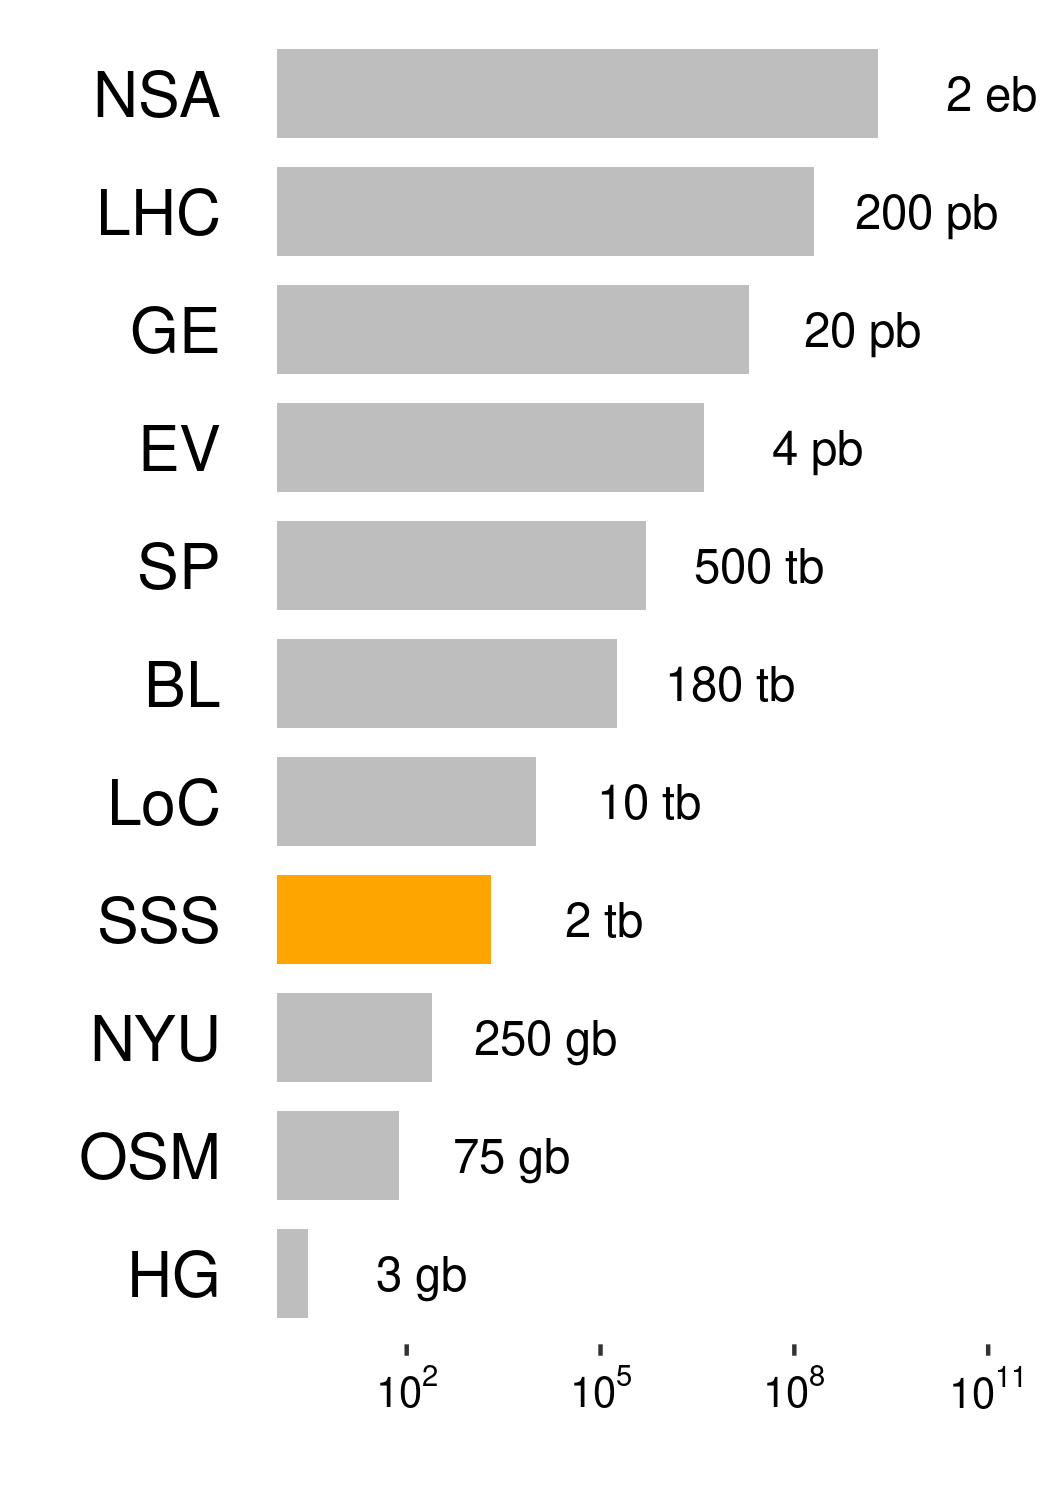
\includegraphics{images/data-size-comparison.png}
  \caption{Comparison of volumes of datasets across various disciplines.}
  \label{figure:toolkit:volume}
\end{marginfigure}

\marginnote[1em]{\fontsize{7}{7}\textit{NSA - National Security Agency, LHC - Large Hadron Collider, GE - Google Earth, EV - Event Horizon project, SP - Spotify music, BL - British Library data store, LoC - Library of Congress, SSS - Smart Street Sensor, NYU - New york city Uber trips 2009-15, OSM - Open Street Map and HG - Human Genome Project}}


%------------------------------------------------------------------------------%

\vspace{1.5em}\noindent\textit{Velocity}\vspace{0.5em}

Velocity is the rate at which the data is collected over time.
It is significant when evaluating big data since some data which may not scale in terms of absolute volume but the speed at which they are received makes them challenging to deal with.
A perfect example is the comparison between data generated by the Large Hadron Collider project by European Council for Nuclear Research and a world wide social network such as Facebook.
Though their total volumes are comparable at 200 petabytes, the data from LHC is generated in concentrated experiments at a rate of 3 petabytes in 5 seconds while Facebook generates the same about in about a day or two.
Since the size of an individual Wi-Fi probe request doesn't vary widely, we define the velocity of this dataset as the number of requests received at a given location at a given location within a given time interval.
Though the precision of the time measured during data collection is in microseconds, the practical data transfer resolution in all the datasets is around 5 minutes.
Hence we measure velocity of out datasets in terms of number of requests every 5 minutes.
Table \ref{table:toolkit:velocity} compares the datasets we collected on Wi-Fi probe requests in terms of their volume.

\begin{table}[h]
  \footnotesize
  \begin{center}
    \begin{tabular}{lcccc}
      \toprule
      Study & Maximum* & Minimum* & Average* & Total** \\
      \midrule
      Pilot Study & 8577 & 188 & 3469 & 3.20 \\
      Main Study & 1362 & 534 & 782 & 0.72 \\
      Smart Street Sensor & 5024 & 6 & 408 & 0.27 \\
      \bottomrule
    \end{tabular}
  \end{center}
  \caption{Comparison of velocity or speed of the datasets of Wi-Fi probe requests.}
  \label{table:toolkit:velocity}
\end{table}

\marginnote{\textit{* Measured/ Estimated for each location in number of requests per 5 minutes. ** Measured/ Estimated for 920 locations in Millions of requests per 5 minutes} }

We observe that locations can receive up to 8500 requests in 5 minutes or can get no request at all depending on the time and how busy it is.
But we can see that on average a national scale project with around 900 locations generates around a million requests every 15 mins. 
Compared to the LHC's 180 billion records or Google's 190 million searches per 5 minutes this seems to be not high speed data.
However, this is much faster compared to traditional data sources such as census or geographical surveys which are updated anywhere between 6 months to 10 years.

To summarise, in terms of velocity, the Wi-Fi probes data can be described as 'Medium' at best. 
The methods dealing with the data should be time sensitive and be able to deal with a continuous stream of data but at the same time need not be real time or need sub-second latency.
Since the Wi-Fi probe requests don't have actual location information the mobile devices, it does not have the similar value in real-time analytics as shown in comparable location or movement based datasets.

%------------------------------------------------------------------------------%

\vspace{1.5em}\noindent\textit{Variety}\vspace{0.5em}

Variety is defined by the amount of variance in the type and characteristics of the data.
Since variety is hard to quantify and compare across disciplines we evaluate the dataset subjectively for the variety present in it.
The data transmitted in a Wi-Fi probe request is defined by the 802.11 Wi-Fi specification \cite{ieee2016} and every probe request has to have a set of mandatory fields for Wi-Fi to work.
This set of fields is the same everywhere across the world and the specification, especially the probe request part, has remained stable over years.
Though there is some variability allowed within the specification, being part of a global standard, the data collected is heavily structured in general.

The first set of variety present in the Wi-Fi probes data set arises from the 'information elements' part of the probe request.
The structure of a probe request is discussed in detail in the data collection chapter and is summarised in Figure ?.
Essentially the information about the capabilities and type of the mobile device is encoded in the information elements part of the probe request and this information is optional and is implemented at the discretion of the manufacturers.
As this information elements are demonstrated to be useful in successfully fingerprinting the mobile devices \cite{vanhoef2016}, mobile devices increasingly don't include any information in them.
Emergence of manufacturers with large market share and narrow set of device models such as Apple and Samsung also reduce further variability in them.
The second set of variety in the dataset arises from the rate at which these probe requests are generated by the mobile devices. 
Unlike devices which generate data on events or at regular intervals, mobile phones generate probe requests at a rate based on various factors.
Though this leads to some challenges in counting footfall from these probe requests the variability exhibited here is neither so large nor so complex that traditional methods could not deal with them.

Comparing with some of the big data encountered in unstructured data collected over web such as social networks or other sensor based methods, the variability here can be considered trivial.
Further when we convert these probe requests in to footfall counts, the variety in the dataset drops almost to zero as it becomes just an ordinal data point varying in geography and time.
Summarising the above, we can confidently say that the Wi-Fi probe request data does not exhibit any `big data' properties in the variety dimension.

%------------------------------------------------------------------------------%

\vspace{1.5em}\noindent\textit{Veracity}\vspace{0.5em}

Veracity is defined as the amount of abnormality present in the data in the form of inaccuracies, biases and noise.
Similar to variety, veracity is hard to quantify hence required a subjective evaluation.
Being sensor collected data, veracity is the dimension where the data exhibits most `big data' properties.


\begin{marginfigure}
  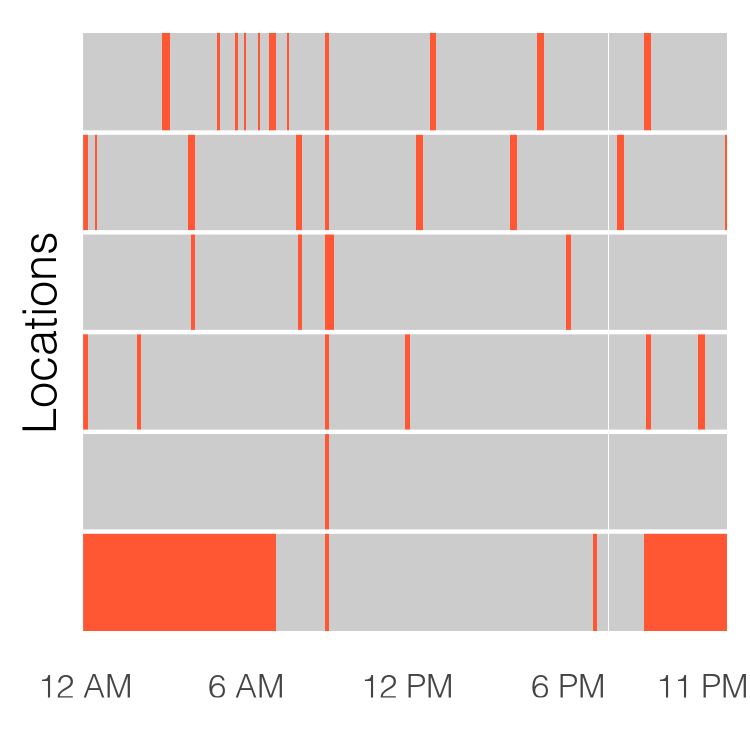
\includegraphics{images/data-veracity-gaps.png}
  \caption{Missing data from five locations at Tottenham Court Road, London on 15 January 2018 demonstrating the veracity of the data.}
  \label{figure:toolkit:veracity:gaps}
\end{marginfigure}

First set of veracity in the dataset arise from the fact that it is collected through sensors located in multiple locations which communicate to the central server using 3G mobile data connectivity.
We know from experience that the sensors are unreliable and fail to send back data regularly due to various reasons.
More over the sensors are installed and uninstalled regularly as partners join and leave the project.
This results in a data stream which is often erratic and incomplete with large gaps in them.
In addition to this the sensors need to be rebooted regularly due to issues or updates leading to small gaps as well.
Since the sensors are part of retail establishments they can be switched on and off regularly in some of them as well.
Figure \ref{figure:toolkit:veracity:gaps} demonstrates the veracity of the data in terms of missing data for a sample of locations in London.
All the above pose immense challenges when we attempt to aggregate the data where we have to estimate and fill these gaps.

There is also a lot of variability in the physical location of the sensors and the area of measurement.
The sensors may report higher or lower count due to their configuration and the context of their location as discussed in chapters pertaining to data cleaning.
This leads to a situation where the accuracy of the data collection varying quite widely across location and times \cite{lugomer2017}.
It is often not clear if the change in the data is due to actual changes at the location or just the change in the configuration of the device.
For example, Opening of a mobile shop next door to the sensor can increase the estimated footfall without any change in actual footfall at the location.

Finally we also have to work within the changing mobile landscape.
Though the Wi-Fi probe requests are standardised by IEEE, the mobile manufacturers have started adopting obfuscation techniques to protect the privacy of the users.
This started with randomisation of MAC addresses, removal of information elements and generally getting more sophisticated with new versions of operating system.
There is also bias in terms of operating system adoption and change in market share between manufacturers.
There is no inherent structure or information on what is changed and how often these changes occur which leads to questions on the continuity of the data over long periods of time.

Summarising from the above, we can confidently conclude that Wi-Fi probe requests dataset shows `Big data' characteristics in terms of its veracity and requires appropriate tools and methods when aggregating, analysing and modelling it.

%------------------------------------------------------------------------------%

\vspace{1.5em}\noindent\textit{Visualisation}\vspace{0.5em}

\begin{figure*}
  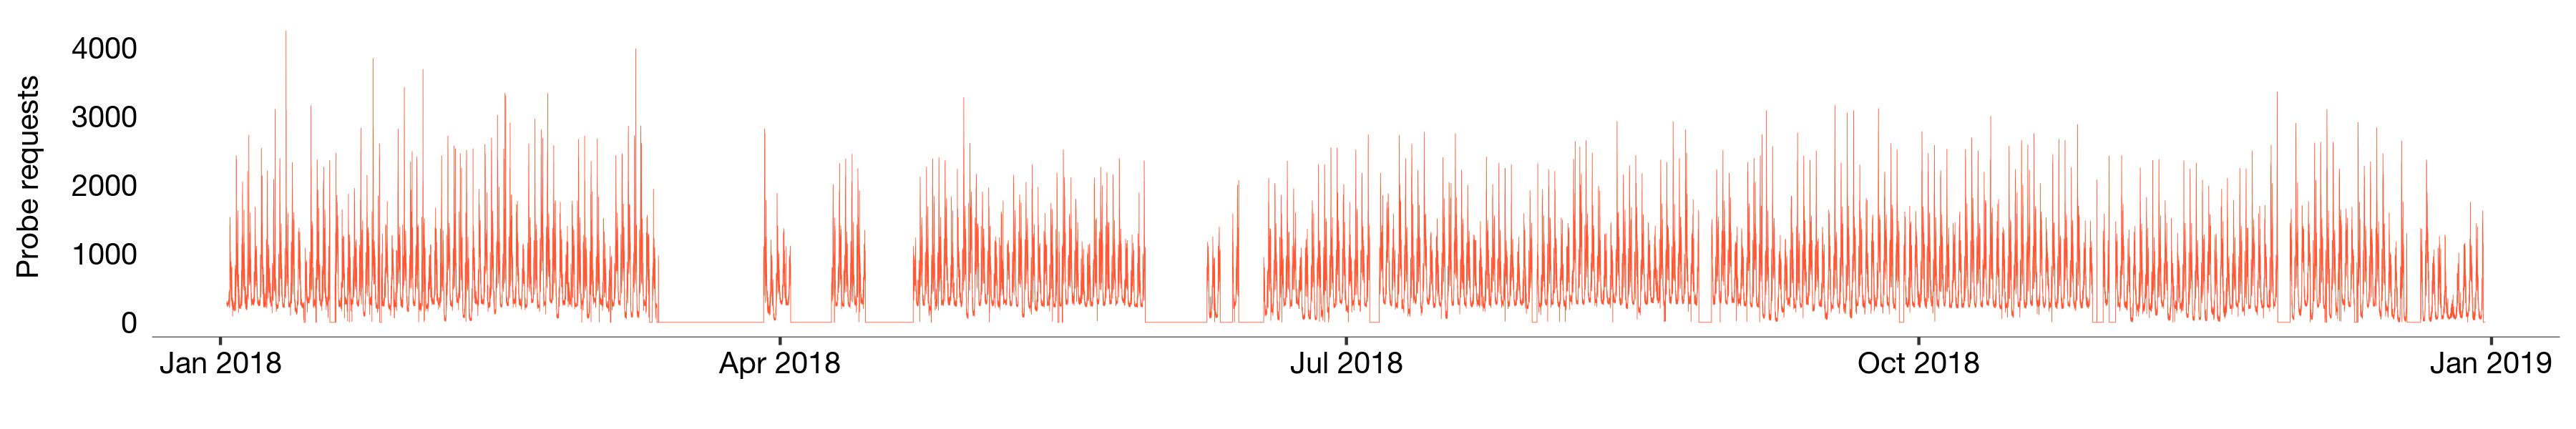
\includegraphics{images/data-visualisation-challenge.png}
  \caption{Number of probe requests collected for every five minute interval at Tottenham Court Road, London on the year 2018 showing the visual complexity of data in the time dimension.}
  \label{figure:toolkit:visualisation}
\end{figure*}

Visualisation is closely related to volume, velocity and variety of the data.
The Wi-Fi data due to its non-trivial volume and velocity, exhibits similar characteristics and challenges in terms of visualisation.
Since there is not much variety in the dataset, when we process the raw data into footfall counts we are left with just the time, location and footfall count for each data point.
Out of these, location and footfall counts are easy to visualise but time exhibits big data properties.
This is primarily due to its granularity at 5 minute intervals and longitudinal nature of the data collection.
The major challenge with Wi-Fi data is to simplify and visualise them in a legible way while showing change in term of time.
The veracity of the data presents challenges in simplifying them and the volume poses challenges in maintaining legibility.
We also have to take the `near real time' aspect of the data into consideration while visualising them.
There is a clear need for always on, interactive, real time dashboards with geographic capabilities in addition to the capabilities of traditional desktop GIS.
There is also need for multiple linked dynamic visualisation platform for separating the scope of the visualisation into manageable units.
Figure \ref{figure:toolkit:visualisation} demonstrates the illegibility of simple visualisations of the data due to granularity, variability and veracity.
We can safely say that the Wi-Fi probe requests dataset is at best `Medium' in the visualisation dimension.

Summarising the above discussion, we can conclude that the datasets collected from Wi-Fi probe requests are at best of 'medium'.
They show the most big data characteristics in terms of their veracity.
In rest of the dimensions the datasets are not truly big data and we need to look at tools and methods appropriate to their size.
The toolkit we devise need to be able to deal with their mid-size volume, velocity and visualisation dimensions and at the same time need to able to deal with the large amount of veracity of in them.
Figure \ref{figure:toolkit:spider} illustrates the summary our discussion.
This leads us to devise a `medium data toolkit' which can be used without incurring the extra cost and complexity introduced by big data tools while be able to handle the data at hand.

\begin{marginfigure}
  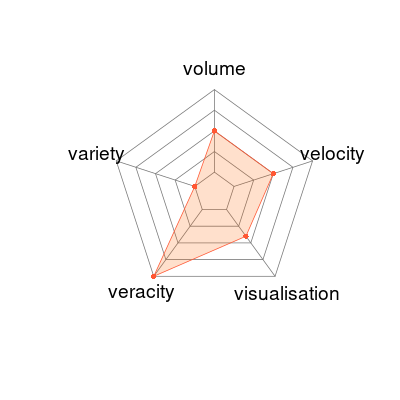
\includegraphics[trim={2.1cm 0 0 0},clip]{images/data-toolkit-spider.png}
  \caption{Big data characteristics of the Wi-Fi probe request datasets in their corresponding dimensions}
  \label{figure:toolkit:spider}
\end{marginfigure}

%------------------------------------------------------------------------------%
% A survey of all tools and methods dealing with big data.
%------------------------------------------------------------------------------%

\subsection{A Survey of Methods and Tools}

Having classified the Wi-Fi probes dataset as a `Medium' sized data, in this section, we survey the tools and methods available at various stages of the data processing and management process - data collection, storage and retrieval, processing and analysis, visualisation.
We first survey the tools available in each stage and specifically look at their suitability for Wi-Fi probe request datasets in terms of the following characteristics,

\begin{itemize}
  \setlength{\itemindent}{1em}
  \itemsep-0.25em
  \item \textit{Performance} - How much data can be processed in a given time?
  \item \textit{Flexibility} - How easy it is to change the scale and scope?
  \item \textit{Complexity} - How many components or parts are involved?
  \item \textit{Cost} - How much money or infrastructure do they require?
\end{itemize}

We then discuss the principles of UNIX philosophy and how it helps in solving similar sized problems in computer science. Finally we pick and connect the tools to devise our toolkit which is best suited for out Wi-Fi probe request dataset.

%------------------------------------------------------------------------------%

\vspace{1.5em}\noindent\textit{Collection}\vspace{0.5em}

We discussed various technologies used in collecting passive data on ambient population and pedestrian movement in the literature search.
In this section we look at tools and methods used to collect Wi-Fi based data passively.
The primary considerations for evaluating data collection strategy are the scale of the infrastructure, expertise and effort required to implement it and cost involved.

There have been numerous sensors, tools and associated software platforms made available for data collection under the umbrella of `internet of things'.
We start by looking at different approaches in the Wi-Fi data collection tools and try to reason the most appropriate solution for our research.
On one end there are low level and low cost bespoke solutions which require lot of effort to implement and maintain.
On the other end there are turn key solutions which doesn't require lesser effort but costs considerably more.
The key is finding a balance between both while satisfying the requirements of the project.
Since the Wi-Fi data is medium sized in terms of volume and velocity, we can deal with solutions with less than optimal scalability but since the data is 'big' in terms of veracity the toolkit has to give us most flexibility. 
Essentially, we are looking for a data collection methodology which prioritises flexibility and cost while performing moderately in terms of scalability and complexity as illustrated in Figure \ref{figure:toolkit:collection}.


\begin{table}[h]
  \footnotesize
  \begin{center}
    \begin{tabular}{lp{5cm}}
      \toprule
      Type of solution & Examples\\
      \midrule
      Bespoke & Micro-controllers with Wi-Fi modules e.g. Audrino + ESP8266\\
      Turn-key & End to end commercial services e.g. Blix, Euclid, Pygmalios etc.\\ 
      \textbf{Ideal} & \textbf{General purpose hardware e.g. Raspberry Pi, Repurposed mobile devices - Tablets, Phones etc.}\\
      \bottomrule
    \end{tabular}
  \end{center}
  \caption{Examples of different types of Wi-Fi based data collection solutions.}
  \label{table:toolkit:collection}
\end{table}

In terms of hardware, an example of a highly customised solution would be a micro-controller, such as Audrino, coupled with dedicated Wi-Fi module and programmed with custom software to collect the exact data needed.
Designing and implementing of such system is time consuming, cumbersome and usually involves significant cost but it can also be highly flexible, efficient and cheap to deploy.
On the other end of this spectrum, we have end-to-end solutions such as Blix, Walkbase, Ecuclid, Retail next, pygmalios etc. where the data is collected through multiple sensors and sources and syndicated into a clean footfall information by a third party service provider.
These platforms for footfall data collection and analysis have the advantage of being quick and easy to develop and deploy while they can also be highly inflexible for changes and turn out to be costly when scaled up.
A middle ground here is to use a general purpose hardware such as single board computers or repurposed mobile devices, augment them with additional hardware modules and use general purpose scripting languages to write software for them.
This way we avoid low level hardware or software design and implementation while maintaining good amount of flexibility.
Table \ref{table:toolkit:collection} shows some examples of such systems while highlighting an ideal system.

\begin{marginfigure}
  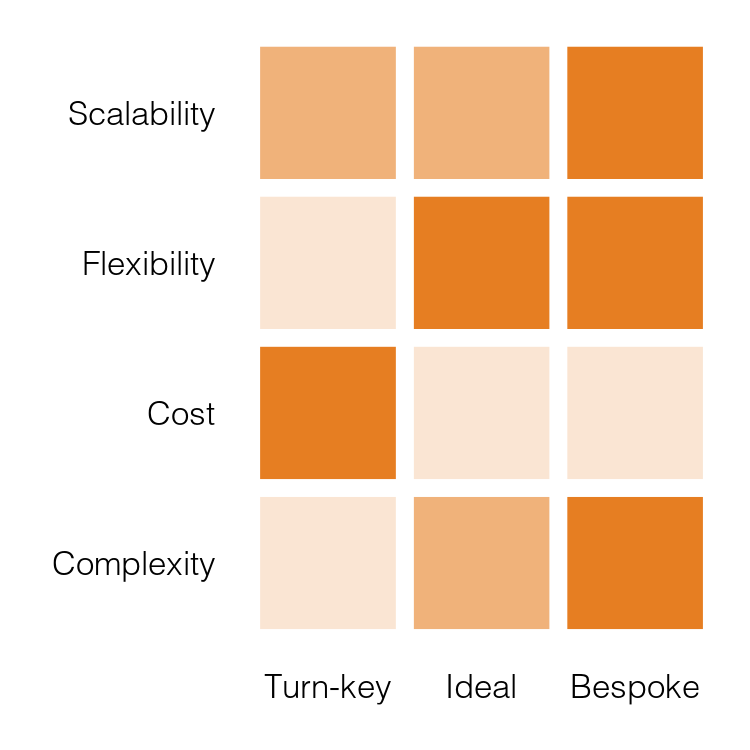
\includegraphics[trim={0.2cm 0 0 0},clip]{images/data-toolkit-collection.png}
  \caption{Characteristics of types of Wi-Fi data collection tools at each end of the spectrum compared to an ideal candidate  }
  \label{figure:toolkit:collection}
\end{marginfigure}
\marginnote[0.1cm]{\textit{(Darker colors show higher score)}}

The Smart Street Sensor project uses its own proprietary sensor system designed and instrumented by the data partner.
The design and implementation decisions were made with the commercial application in mind and is not entirely relevant to our discussion in the context of our research.
For the research conducted with the data, it is necessary to understand the data collection process and make sure it aligns and integrates with the rest of the toolkit.
As discussed in the data collection chapter, the methodology used in the smart street sensor project satisfies our requirements.
The toolkit we designed to collect other datasets are in-part inspired by this methodology or a modified version to include more flexibility.
The toolkit consists of Raspberry Pi, Linux, tcpdump or tshark \cite{wireshark2} and nodejs.
Raspberry Pi and the Linux OS provides a general purpose base system and hence the flexibility.
On top of this we built our data collection system by assembling open source and free network analysis tools such as tcpdump and tshark along with other tools providing functions such as scheduling, personal data obfuscation and data transmission with scripting languages like nodejs and bash.

%------------------------------------------------------------------------------%

\vspace{1.5em}\noindent\textit{Storage}\vspace{0.5em}

Data storage technology is one of the most diverse landscape in terms of both methods and tools available.
It has been constantly in research and development since the beginning of computing and is one of the fastest changing landscapes with the advent of big data paradigm.
A comprehensive review of storage solution warrants a chapter in itself so we restrict our survey to an outline of most significant approaches and corresponding systems and tools.

At one end of the spectrum is one of the most underappreciated for of data storage - File systems.
Though they seem like a low level interface for storing data, file systems have their advantages as well.
When the data is not complex or inter-related, flat text files in file systems could be the fastest way to store, search and retrieve data.
Since operating systems are usually optimised to manage storage media through file systems, they involve no additional overhead and are extremely reliable.
The hierarchical file systems use in most of the operating systems act as an index with hierarchical data.
The major disadvantage of file systems is that they are not useful for managing data with any kind of complexity.
This is the primary reason why database management systems are developed on top of file systems.

Database systems can be broadly divided into relational and document based.
The relational databases are optimised to deal with relational data and usually enforce strict structure for the data
In general they can handle large number of rows and are designed to scale vertically.
Most relational database systems try to guarantee ACID \sidenote[][-7cm]{Atomicity, Consistency, Isolation and Durability are properties which make sure that the data in the database is valid even during failures.} compliance and hence used in critical systems such as financial operations, sales etc \cite[-5cm]{Haerder1983}.
The document based databases are optimised to deal with unstructured data and can doesn't need a strictly defined scheme.
In general they can handle large number of columns and are designed to be distributed and scaled horizontally.
Being distributed, most document based databases try to pick a focus and compromise on others as specified in CAP theorem \sidenote[][-3cm]{Brewer's theorem or CAP theorem states that it is impossible to simultaneously guarantee consistency, availability and partition tolerance in a distributed data store.}.
There a numerous databases systems which prioritise different things and the right solution depends on the properties of the data and the requirements of the project.

Since the publication of the paper on `Google file system' by google \cite{sanjay2003}.
There have been significant effort in designing and building 'big data' file storage systems which can large data in the range of petabytes.
These systems are designed to be distributed and optimised for high throughput for queries on them.
Hadoop Distributed File System (HDFS) is one such file system which is also the most widely adopted.
There are numerous cloud based, third-party solutions built with these file systems making them easy to use.
There are also numerous tools, libraries and frameworks which emulate the features of database systems on these distributed file systems making them easier to use further.
The primary advantage of these systems is the sheer scalability they provide when it comes to data volume.
The primary disadvantage is the associated overheads in terms of cost and time incurred in learning, designing and implementing them.
Unless the project is sufficiently large, the advantages gained usually do not justify the overheads introduced.
Table \ref{table:toolkit:storage} summarises the above discussion along with relevant examples.

\begin{table}[h]
  \footnotesize
  \begin{center}
    \begin{tabular}{lcp{2cm}p{4.5cm}}
      \toprule
      Approach & Data size & Examples & Comments\\
      \midrule
        File system &
          \textless{} 10 TB &
          ext, ntfs, zfs, btrfs &
          Simple and efficient. Best for hierarchical data. Cannot handle complex connected data.\\
        \addlinespace[0.2cm]
        Relational DB &
          \textless{} 5 TB &
          MySQL, PostgreSQL&
          Handles structured and relational data. Optimised for large amount of rows and tries to guarantee validity.\\
        \addlinespace[0.2cm]
        Document DB &
          \textless 10 TB &
          MongoDB, Cassandra&
          Handles unstructured data. Optimised for large number of fields and distribution to multiple clusters. Tries to focus on any two guarantees of the Brewer's theorem.\\
        \addlinespace[0.2cm]
        Distributed FS &
          \textgreater{} 10 TB &
          HDFS, Ceph, GFS &
          Optimised for really large datasets which need to be distributed over multiple nodes.\\
        \addlinespace[0.2cm]
        Cloud Storage &
          \textgreater{} 10 TB &
          AWS, Azure, SWIFT &
          Implements distributed file systems on the cloud. Has more reliability and scalability than local implementations.\\
        \addlinespace[0.2cm]
        Data Warehouse &
          \textgreater{} 10 TB &
          Hive, Hbase, Impala, Presto&
          Interfaces built on top of distributed file systems to emulate capabilities of relational databases on them.\\
      \bottomrule
    \end{tabular}
  \end{center}
  \caption{Various data storage approaches and their characteristics.}
  \label{table:toolkit:storage}
\end{table}

We saw that the Wi-Fi probe request datasets are `Medium' sized hence we can safely eliminate distributed file systems for storing them.
Though the smart street Sensor project uses Azure Blob Storage, when the data is downloaded to the local servers at the university, we can just store them in the file system because of their size (2TB approx.) and the hierarchical nature.
The folder structure of - year/month/day/location/interval/ with individual text file, enable us to query the data for any given location at any interval nearly instantaneously without any further database operations.
When this raw data is processed into 5 minute counts, we require more relational queries.
For this purpose a relational database is sufficient as volume is quite small (25GB approx.).
We chose PostgreSQL because of the PostGIS extension which gives us flexibility in handling geographic data.

%------------------------------------------------------------------------------%

\vspace{1.5em}\noindent\textit{Processing}\vspace{0.5em}

\begin{marginfigure}
  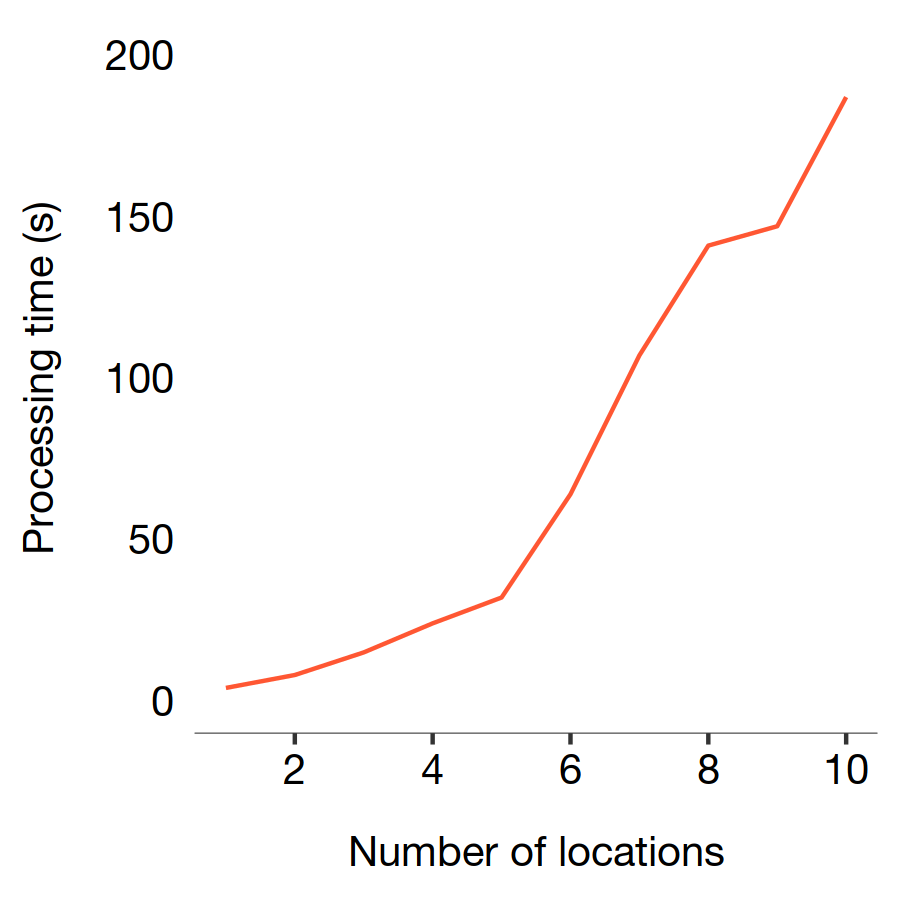
\includegraphics[trim={0 0 0 0},clip]{images/processing-time-old.png}
  \caption{Exponential increase in the processing time when using traditional methods.}
  \label{figure:toolkit:time:old}
\end{marginfigure}

\marginnote[1em]{\fontsize{7}{7}\textit{The processing involves parsing JSON data received for a single day at each location and aggregating them as number of probes requests received in every five minute intervals.}}

We saw that the data is medium in terms of volume and velocity and shows big data properties in terms of veracity.
Hence we require tools which are capable of dealing with the veracity of the data while being able to manage the volume and velocity.
The traditional approach to deal with such dataset is to load it into a general purpose analysis tool such as R or a GIS packages and process it.
The size of the dataset and the lack of meaningful complexity of geography element in the data eliminates the use of GIS packages.
Scripting languages such as R and Python can deal with the dataset and its requirements but the time taken to do so increases exponentially with the size of the data as the size of objects in memory increases.
Figure \ref{figure:toolkit:time:old} illustrates the increase in processing time with respect to number of location for a simple exercise where a day's worth of raw data is parsed and aggregated into number of probe requests per 5 minute intervals 
(The code used to produce these benchmarks are detailed at Section \ref{appendix:benchmark}).
This becomes prohibitively expensive as the number of locations and complexity of the processing increases.
Though this can be improved with more efficient coding practices, the margin of improvement is quite limited hence creating the need for better techniques.
It is important to note that data processing is done in two stages - the first stage where the raw Wi-Fi probe requests are filtered, cleaned and aggregated into footfall counts and second stage where the footfall counts are in turn analysed to produce reports and visualisations.
The traditional methods are sufficient for the second stage of the processing and the first stage is the one which requires a better solution.

On the other end we have big data analysis tools which are built for dealing with extremely large amount of data.
Since the publication of the paper on MapReduce, there have been immense developments in the Big data analysis landscape.
There numerous distributed programming tools to use the data stored within a distributed storage system each focussing on specific type of data and analysis.
A concise, non-comprehensive list of types of data or specialities and corresponding big data tools is shown in Table \ref{table:toolkit:processing}.

\begin{table}[h]
  \footnotesize
  \begin{center}
    \begin{tabular}{lp{3cm}}
      \toprule
      Tools & Speciality\\
      \midrule
        General purpose & MapReduce, Spark\\
        Real-time streams & Flink, Pulsar\\
        Events or messages data & Storm, Kafka, Flume\\
        Networked or graph data & Tinkerpop, Corona \\
        Scheduling & Oozie, Falcon, Azkaban\\
        Turn-key platforms & SpringXD, Cask Data\\
      \bottomrule
    \end{tabular}
  \end{center}
  \caption{Various types of big data processing tools and corresponding examples.}
  \label{table:toolkit:processing}
\end{table}

We can rule out the necessity of the above big data tools since our dataset is neither big enough nor fast enough.
The dataset does not have any specialised structure such as graph or network but just a very minimal component of geography to it.
Using any of specialised big data tools is just going to introduce immense overheads without any added benefits.
We need something in-between the above two approaches where we is sufficiently fast and flexible for our datasets.

This is where we come across the possibility of using standard Unix tools along with connecting them to create a processing pipeline.
In some cases, a data processing pipeline made using command line Unix tools have been demonstrated to be 230 times faster than using big data toolkits \cite[-2cm]{adam2014}.
The command line tools were developed as parts of Unix operating system for processing text. 
They are developed in line with the Unix philosophy which focuses on modular and minimal software development. 
The core tenants of the Unix philosophy has been summarised by Doug McIlroy as below,\cite{mcilroy1978},

\begin{enumerate}[rightmargin=1cm]
  \setlength{\itemindent}{2em}
  \itemsep-0.25em
	\item Make each program do one thing well. To do a new job, build afresh rather than complicate old programs by adding new "features".
	\item Expect the output of every program to become the input to another, as yet unknown, program. Don't clutter output with extraneous information. Avoid stringently columnar or binary input formats. Don't insist on interactive input.
	\item Design and build software, even operating systems, to be tried early, ideally within weeks. Don't hesitate to throw away the clumsy parts and rebuild them.
	\item Use tools in preference to unskilled help to lighten a programming task, even if you have to detour to build the tools and expect to throw some of them out after you've finished using them.
\end{enumerate}

\begin{marginfigure}
  \forcerectofloat
  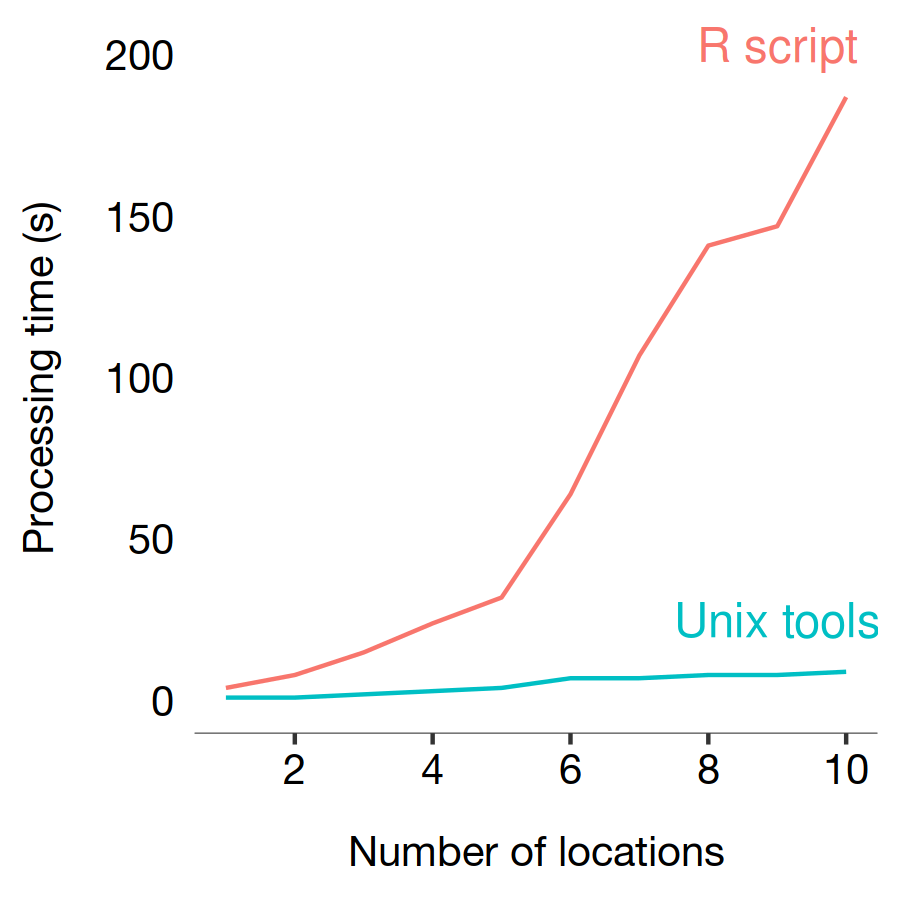
\includegraphics[trim={0 0 0 0},clip]{images/processing-times-r.png}
  \caption{The increase in processing time with the Unix pipeline is linear thus improves the scalability compared to R based processing}
  \label{figure:toolkit:time:new}
\end{marginfigure}

These principles along with the `pipe' operator gives us necessary tools to build more complex tools.
We can replace most of the libraries we used in the R implementation of our processing with a corresponding command line tools and connect them together with a text interface to achieve similar pipeline.
The first advantage of such design is that it is much more efficient than a monolith design.
These tools being actively developed for since their invention are compiled as native binaries and are usually extremely optimised resulting in a much faster pipeline.
Because of the design of the pipe operator, the individual parts of the pipeline are executed in parallel as chunks of data are passed through them thus avoiding the need to load entire datasets into memory which results in an exponential increase processing time with the size of the data.
Being modular, we can even introduce process level parallelism to parts of the pipeline without any major change in the overall design.
Finally the modular structure also gives us the advantage of using the best tool for any part of the pipeline.

\begin{table}[h]
  \footnotesize
  \begin{center}
    \begin{tabular}{p{4cm}p{3cm}p{3cm}}
      \toprule
      Tools & R Library & Unix tool(s)\\
      \midrule
        Move data to and from Azure blog storage, SQL server and Postgres & AzureR, odbc , RPostgreSQL & azcopy, mssql, psql\\
				Convert data from JSON format to CSV & jsonlite & jq\\
        \addlinespace[0.2cm]
				Encrypt raw data for secure storage & Rcrypt & gnupg\\
        \addlinespace[0.2cm]
				Anonymise personal data into cryptographic hash & digest & openssl\\
        \addlinespace[0.2cm]
				Transform and manipulate tabular data& dplyr & find, cat, cut, grep, sed, awk, sort, uniq, column, paste, join\\
        \addlinespace[0.2cm]
				Impute missing value using time series analysis & imputeTS & Rscript\\
        \addlinespace[0.2cm]
				Visualise the results into maps and charts & ggplot2 & Rscript\\
        \addlinespace[0.2cm]
        Create and manipulate geographic data & sf, rgdal & postgis, gdal\\
      \bottomrule
    \end{tabular}
  \end{center}
  \caption{Tasks in the processing pipeline, corresponding R libraries and equivalent Unix tools}
  \label{table:toolkit:tools}
\end{table}

\begin{marginfigure}[2cm]
  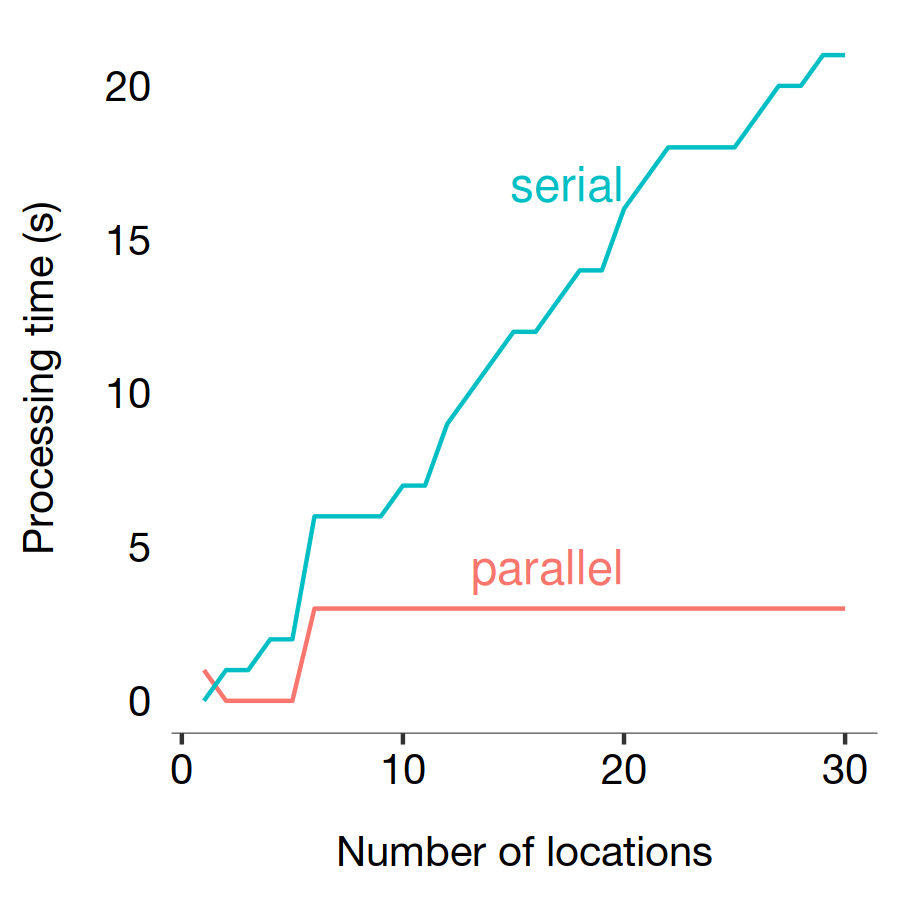
\includegraphics[trim={0 0 0 0},clip]{images/processing-times-parallel.png}
  \caption{The scalability of the processing pipeline could be further improved with parallelising it.}
  \label{figure:toolkit:time:parallel}
\end{marginfigure}

All of the gives us an extremely minimal and efficient toolkit to process the raw Wi-Fi probes data into counts in a scalable way.
Figure \ref{figure:toolkit:time:new} compares the processing times of such Unix toolkit with the traditional R based toolkit as the data size increases.
We can see that Unix toolkit performs extremely well and the performance gains are significant as the size of the data increases.
For example, to process data for 25 locations, R based toolkit takes around 20 minutes while the Unix toolkit gets it done in 20 seconds 
(The code used to produce these benchmarks are detailed at Section \ref{appendix:benchmark}).
Table \ref{table:toolkit:tools} shows the activities in our pipeline and corresponding libraries in the traditional R workflow along with the equivalent Unix tools.
It is important to note that tools for doing specialised actions such as statistical analysis, machine learning and time-series analysis are built on top of scripting languages such as R and Python.

These can be embedded into our Unix pipeline as scripts running in corresponding front-ends such as Rscript or python.
This toolkit can be further accelerated by parallelising parts of the pipeline using gnu-parallel \cite{tange2018}.
For example, the previous example pipeline can be parallelised by spawning a pipeline for each location this reduces the processing time for a set of 25 locations from 18 seconds to 3 seconds.
This done by utilising every processor cores available in the CPU.
Figure \ref{figure:toolkit:time:parallel} compares the processing times of the Unix toolkit with a parallelised implementation (The code used to produce these benchmarks are detailed at Section \ref{appendix:benchmark}).
Finally all the Unix tools discussed in this toolkit are open source and free software which has almost no cost in terms of resources.
Since these tools are part of the POSIX specification \cite{walli1995} for operating systems, the expertise in their design and use are transferable to and from other disciplines thus reducing researcher time learning and using these tools.


%------------------------------------------------------------------------------%

\vspace{1.5em}\noindent\textit{Visualisation}\vspace{0.5em}

In the last section we saw that the visualisation dimension of the data shows some level of complexity.
The primary source of this complexity arises from the longitudinal nature of the data and the noise due to granularity of the data.
For the processed dataset, traditional visualisation and mapping libraries with R is sufficient while the visualisation of raw data across long time periods for either for exploratory analysis or for communication needs some form of interactivity or simplification to be able to legible.
Data driven documents (D3) \cite{stanford2011} and Dimensional charting (DC) provides us with both of these requirements.
Both of these tools can accept text based input and can fit with other Unix tools discussed earlier.
In case of binary file output such as images or documents, they could be directed to the file system and then read into other programs.

%------------------------------------------------------------------------------%
% Final summary and conclusions
%------------------------------------------------------------------------------%

\subsection{The Bespoke `Medium data toolkit'}

In this chapter we saw how the advent of internet and internet enabled devices has lead to significant increase in the amount of data generated and collected across disciplines. 
This data deluge and improvements in the capabilities of computing hardware has fuelled an explosion of research and development in tools and methods to deal with these `Big data'.
Though these big data tools promise huge improvements in processing capabilities, when used under wrong circumstances they can lead to unwanted overheads and costs.
Thus we need a framework to examine and understand the scale of the data that is being used so that we use the right tools for the right purposes and the 5Vs of `Big data' - Volume, Velocity, Veracity, Variety and Visualisation provides us with such frame work.
Every dimension of big data poses unique set of challenges and we need make right decisions in choosing specialised tools and methods to overcome them.

We then closely examined the Wi-Fi probes data we collected with this framework and found that the data, though posed significant challenges with traditional data processing techniques, do not exhibit `big data' properties in all its dimensions. 
Only veracity of the data was found to have any meaningful big data properties, while volume and velocity was found to be 'medium' at best. 
The datasets lacked any variety and posed minimal challenge in the visualisation dimension because of it high temporal granularity.
Thus we arrived at the requirements for a bespoke `medium data toolkit' which is able to deal with these challenges.

\begin{figure}
  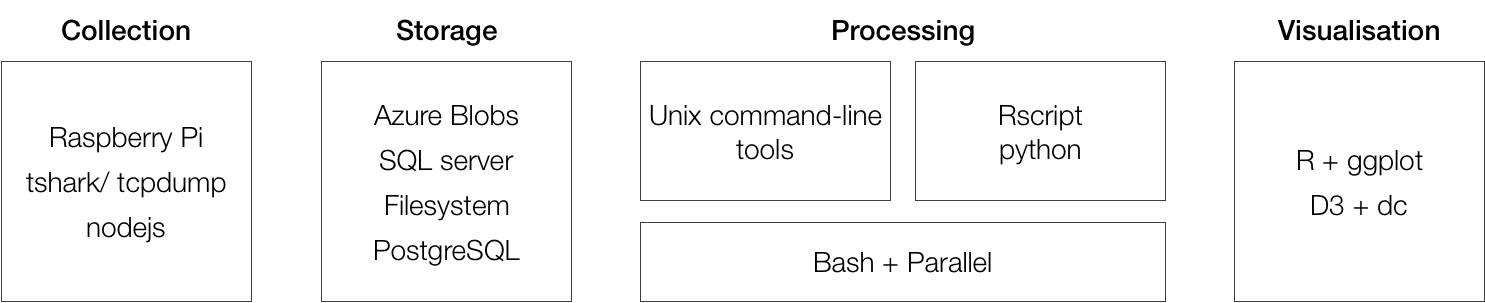
\includegraphics{images/toolkit.png}
  \caption{Outline of the `Medium data toolkit' devised to collect, process, visualise and manage the Wi-Fi probe requests data}
  \label{figure:toolkit}
\end{figure}

We undertook a brief survey of tools available for collecting, storing, processing and visualising the Wi-Fi probe request data and with the understanding of the data from the previous analysis chose the ones which are perfect for the datasets.
For collecting Wi-Fi probes data in a scalable way, we chose a general purpose single board computers such as Raspberry-Pi along with open source tools such as tcpdump and tshark in a Linux environment.
For data storage we narrowed in on using just the file system for the raw data and relational database management system for the processed counts.
To process the raw data we chose to devise a processing pipeline using an assortment of standard Unix command line tools linked together using a shell scripting language and parallelised at the process level with gnu-parallel.
We also demonstrated that this processing pipeline can be 400 times faster than the using a monolithic pipeline even with a small sample of locations.
For visualisation we chose D3 and DC as the solution for communicating time information legibly.
Finally we arrive a `medium data toolkit', illustrated in Figure \ref{figure:toolkit}, which is best suited for the Wi-Fi probes dataset which we employ to process and examine the data further.


\cleardoublepage
\section{Device fingerprinting}

In the past decade, Wi-Fi has emerged as one of the most commonly used technologies in providing high speed internet access to mobile devices such as smartphones, tablets and laptops in public and private spaces \citep{torrens2008}.
This has resulted in multiple Wi-Fi networks being available at almost every location in dense urban environments.
Traversing through this overlapping mesh of Wi-Fi networks, modern mobile devices with Wi-Fi network interfaces regularly broadcast a special type of signal known as `Probe Requests' in order to discover the Wi-Fi networks available to them.
This helps these devices to connect and switch between the Wi-Fi networks seamlessly.

Probe requests are low level signals standardised by IEEE 802.
1 specification \citep{ieee2016} for service discovery, and are implemented in any Wi-Fi capable device irrespective of the manufacturer or the model.
This ubiquity and standardisation makes them an excellent source of open, passive, continuous, and wireless data generated by Wi-Fi capable devices present at any given time and location.
Considering the unprecedented levels of mobile device ownership in recent years, we can, in turn use this data to understand the population distribution in highly dynamic urban environments with high spatial and temporal granularity \citep{freud2015, konto2017}.
While a Wi-Fi based method to collect data offers us various advantages such as, easy scalability and efficiency in terms of cost and time, it also introduces few systematic biases and uncertainties in the collected data along with the serious risk of infringing on the privacy of the mobile users.
In this section, using the set of probe requests and manual counts collected at various high street locations across London, we demonstrate that pedestrian footfall at these locations can be estimated with considerable precision and accuracy while protecting the privacy of the pedestrians.

Unlike GPS, the location of the Wi-Fi enabled mobile device cannot be directly inferred from Wi-Fi, however there are reliable methods to triangulate the location of mobile devices from the locations of known access points (AP) and the signal strength reported by them \citep{he2003, moore2004, lamarca2005}.
This can overcome the usual shortcoming of GPS, which struggles for precision and accuracy in indoor and densely built environments \citep{zarim2006, kawaguchi2009, xi2010}.
Utilising this, we can easily and quickly estimate trajectories of the mobile devices \citep{musa2012} which can be used similarly to the GPS trajectories to understand individual travel patterns \citep{rekimoto2007, sap2015}, crowd behaviour \citep{abedi2013, mowafi2013}, vehicular \citep{lu2010} and pedestrian movement \citep{xu2013, fukuzaki2014, wang2016}.
Such data can also be used in transportation planning and management to estimate travel time \citep{musa2011} and real time traffic monitoring \citep{abbott2013}.
Using techniques demonstrated by \citep{franklin2006} and \citep{pang2007}, along with information present in the probe requests, one can even model interactions between the users \citep{cheng2012, barbera2013, cunche2014} such as predicting which of them are most likely to meet again \citep{cunche2012}.
Using the semantic information present in these probe requests it even is possible to understand the nature of population at a large scale \citep{di2016}
.

Although extensive research has been carried out on this subject with feasible and favorable results, in recent years, one of the major challenges faced in such attempts has been the increasing attempt by mobile phone manufacturers to protect their users’ privacy by anonymising the globally identifiable portion of the probe requests \citep{greenstein2008}.
Various methods have been devised to overcome this anonymisation process such as estimating the device model information from a known dataset of manufacturers and device behaviours \citep{martin2016}; Scrambler attack using a small part of the physical layer specification for Wi-Fi \citep{vo2016, bloessl2015}; and timing attack where the packet sequence information along with information elements present in the probe request frame is used \citep{matte2016, cheng2016}. A combination of these methodologies has been proven to produce de-anonymised globally unique device information \citep{vanhoef2016, martin2017}. These approaches usually result in serious risk of breach of privacy of the users of the mobile devices by revealing their identifiable personal information.

There is a clear gap in the research for exploring methodologies for estimating the number of unique mobile devices from a set of anonymised probe requests, without the need to reveal their original device information.
Such a technique has various applications such as uncovering the urban wireless landscape \citep{rose2010}, revealing human activity at large scales \citep{qin2013}, estimating pedestrian numbers in crowds \citep{schauer2014, fukuzaki2015}, and even counting people in hyper local scales such as queues \citep{wang2013}.
With enough infrastructure to collect such information we can even aim to generate a real-time census of the city \citep{konto2017}.
With this background, we set out to devise and implement a methodology to reliably estimate human activity such as pedestrian footfall from Wi-Fi probe requests without risking a breach of privacy of the users involved. 

\vspace{1.5em}\noindent\textit{Methodology}\vspace{0.5em}

The primary aim of this research was to enable us to collect a series of probe requests and process them into a usable pedestrian footfall count.
We did this by using a Wi-Fi receiver to collect probe requests broadcast by mobile devices, filtering out the background noise, and aggregating them based on the device that generated them.
In this section, we examine the characteristics of probe requests in detail, devise a methodology to collect these probe requests in public areas, examine the systemic biases and uncertainties in the data collection method, and devise data processing methods to overcome these challenges.
Finally, we compare the processed footfall counts to the ground truth recorded by primary surveys.

Probe requests are a special type of management packet broadcast by Wi-Fi enabled devices as part of their various functions such as scanning for available APs and quick geolocation by triangulation based known APs, etc.
These are broadcast by all Wi-Fi enabled devices regardless of the manufacturer, type or model of the devices, although there is some variation in the frequency and the content of the information transmitted through them.
In some cases, such as Android devices, these are broadcast even when the Wi-Fi functionality has been turned off by the user so that the device can immediately connect to networks when the functionality is switched back on.
Since some devices even use the probe requests as a less accurate form of localisation, they continuously send probe requests when Wi-Fi has been switched off.
Thus, these signals can be used to reliably identify the presence of Wi-Fi enabled mobile devices.
Being a first step of connection initiated by the mobile device, these packets have information regarding the characteristics of the mobile device itself.
Some of the key information we can infer from these requests are,

\begin{enumerate} 
\item \textbf{Media Access Control (MAC) address} which is a name identifying the wireless hardware of the mobile device, 
\item \textbf{Sequence number} of the request for the mobile device to keep track of the responses, 
\item \textbf{Time stamp} at which the request was received by the AP, 
\item Total \textbf{length} of the request in number of bits, and 
\item The \textbf{strength of the signal} received by the mobile device.
\end{enumerate}

The MAC address is the primary identifier for the mobile device and has two parts.
The first part is the Organisationally Unique Identifier (OUI) which provides information about the manufacturer of the device and the second part is the identifier for the device.
In modern devices, to protect users' privacy, the second part of the MAC address can also be randomised and hence may not be unique to devices.
When the MAC address is randomised, it is marked as such by setting a specific bit in the probe request packet as 1.
Although sequence number of the packet is strictly unique to a mobile device, we hypothesize that we can use them to estimate the number of unique devices as demonstrated by \citep{vanhoef2016}; where optional information present in the probe requests - Information Elements (IE) along with the sequence numbers, have been used to fingerprint the devices.
This approach has become increasingly difficult as mobile phone manufacturers have severely limited the IEs present in the probe requests thus leading us to explore methods which use only the sequence numbers.
This also affects the established commercial solutions using Wi-Fi probe requests such as Blix, Walkbase, Euclid Analytics, RetailNext etc.
There has been another solution proposed by \citep{hong2018} where the authors tried to solve the similar problem using a hidden markov models based trajectory inference algorithm but the scope of this research was limited to enclosed, exit controlled public spaces such as shopping malls, railway stations, etc.

Data collection was done with the help of custom sensors built from modifying the hardware used in Smart Street Sensors \citep{sss2016} and updating them with custom software.
The sensor is essentially a Raspberry-Pi device with Wi-Fi and 3G modules.
It keeps the Wi-Fi module in `Monitor mode' and uses the open source software - Wireshark \citep{wireshark2} to passively collect all packets sent to `broadcast', marked with type as `management', and subtype `probe requests'.
The MAC address in these probe requests is obfuscated at the device level using a cryptographic hashing algorithm and transmitted through 3G connection to a central database via web-sockets protocol, where it is stored in a PostgreSQL database for further analysis.
The random salt used in the hashing algorithm was rotated regularly to further mitigate the risk of de-anonymisation of the hash.
Though hashing cannot completely ensure anonymisation as discussed in \citep{demir2014}, it can sufficiently obfuscate the data; which along with a secure process of data handling, gives us reasonable security.
An overall schematic of the data collection and storage process is shown in Figure \ref{datacollection_schematic}.
The ground truth on the number of pedestrian footfall was recorded using a custom Android application - Clicker \citep{bala2018}.
This app logs accurate timestamps each time the surveyor records a pedestrian crossing the designated cordon line at the location.
In addition to counting the pedestrians manually, this procedure results in the device broadcasting probe requests regularly, which in turn, gives us a `known device' to calibrate our methodology against.


% \begin{figure} 
% 	\centering \includegraphics[width=\linewidth]
% 		{images/figure_1.jpeg}
% 	\caption 
% 		{Schematic diagram showing the process of collecting and storing probe
% 		requests using the sensor}
% 	\label{datacollection_schematic} 
% \end{figure}

After collecting data, we began estimating the footfall or pedestrian activity from them by identifying the following potential uncertainties arising from our data collection method:

\begin{enumerate} 
  \item \textbf{Background noise} - since the extent to which Wi-Fi signals travel differs subject to various factors such as interference and humidity, it is close to impossible to restrict our data collection to a finite area of interest.
  This can lead to a significant background noise at certain locations.
  For example, a phone shop or a bus stop located next to the study area can artificially increase the number of probe requests received by the sensor.
  It is important to note that this method may not work effectively on study locations with complex configurations such as the source of noise and the area of study being located at the same distance from the sensor.
  This aspect is explored in detail in the broader case study in the following sections.
  \item \textbf{MAC randomisation} - mobile devices in recent years have been using randomised `local' MAC addresses for probe requests to protect the users from being tracked.
  This makes it impossible to tell if the probe requests are being sent by the same mobile device. This along with the previous problem can further increase the magnitude of error by several fold.
  \item \textbf{Mobile ownership} - since the rate of mobile ownership can vary widely across geography and demography, we cannot assume that every mobile device translates to one pedestrian footfall.
  In addition to this, there is a long term overall increase in mobile ownership which may affect the number of probe requests collected overtime.
\end{enumerate}

We propose the following internal and external validation methods to tackle each of these uncertainties.

% \begin{figure} 
% \centering 
% \subfigure [Distribution of signal strengths (dBm) showing the filtering of
% 		background noise] {\resizebox*{0.45\linewidth}{!}
% 		{\includegraphics{images/figure_2a.jpeg}}}
% \hspace{20pt}
% \subfigure [Clustering probe requests as nodes in a graph using increasing
% 		sequence numbers] {\resizebox*{0.45\linewidth}{!}
% 		{\includegraphics{images/figure_2b.jpeg}}}
% \caption {Schematic diagrams explaining the methods for filtering by signal
% 	strength and clustering using sequence numbers}
% \label{methodology_schematic}
% \end{figure}

\vspace{1.5em}\noindent\textit{Filtering with Signal Strength}\vspace{0.5em}

One of the clues that we can use to estimate the distance between the mobile device and the sensor is the strength of the signal received by the sensor.
The obvious approach was to first try and establish a relationship between the signal strength and distance and to use this to filter out the unwanted probe requests.
However this approach was found to not be feasible, since the decay of signal strength with respect to distance is not always constant.
For instance, signal strength varies with atmospheric conditions, the presence of obstructions between the source and the target, the nature of these obstructions, and the strength (power level) of the source.
This severely limits our ability to establish a simple conversion between reported signal strength and distance.
As such, there was a need for a method which takes in to account all of these variables across the various locations.

We assumed that, in configurations where a specific source of background noise was at a constant distance, there must be a distinct pattern in the number of probe requests reporting signal strength corresponding to that distance.
For example, if there was a phone shop next to our sensor where hundreds of phones regularly sent probe requests, there should be a sharp rise in the of number of probe requests with reported signal strength corresponding to the distance between the sensor and the phone shop, irrespective of the local conditions as shown in Figure \ref{methodology_schematic}.
We could identify these breaks in the data using traditional one dimensional clustering algorithms such as `jenks natural breaks', `k-means', `quantile' and `hierarchical clustering', etc.
Since we were only looking for the break in the data and not for absolute values, the methodology should apply for all the variations due to micro site conditions reducing the overall noise in the collected data.

\vspace{1.5em}\noindent\textit{Clustering with sequence numbers}\vspace{0.5em}

Since our primary unique identifier - MAC addresses are being anonymised by new devices, we needed to find other information present in the probe requests for use as a unique identifier.
The obvious approach was to establish a factor of randomisation, and adjust the counts for the probe requests based on this factor.
We found this approach to not be feasible since the proportion of devices which randomise the MAC addresses increased over time.
There was also a wide variation in the frequency at which the devices randomised the MAC addresses and the method used for the process.
This led us to look for a more generalisable approach which was independent of the device model.
From our initial look at the data, we found that OUI and the sequence number of the packet was the most promising information to achieve this.
First we divided our dataset into sets of probe requests with randomised and non-randomised MAC addresses by looking at the second character of the vendor part of the MAC address; if it was E, A, 2 or 6, then those addresses were identified to be randomised.
We kept the MAC address as the unique identifier for the non-randomised requests and further divided the randomised ones in to sub-categories based on their OUI.
We then  identified unique mobile devices from within those sets, and assigned a unique identifier to each device.

The proposed algorithm created a graph where the probe requests represented the nodes; links were created between them based on the following rules:

\begin{itemize} 
  \item A link could go only forward in time.
  \item A link could go from low to high sequence numbers. 
  \item A link could exist between nodes with a maximum time difference of $\alpha$ - time threshold.
  \item A link could exist between nodes with a maximum sequence number difference of $\beta$ - sequence threshold.
  \item A node could have only one incoming link and one outgoing link, which is the shortest of all such possible links in terms of both time and sequence number.
\end{itemize}

The nodes were then assigned a unique ID based on the unique connected component they belonged to as shown in Figure \ref{methodology_schematic}.
This unique identifier was used in the place of MAC addresses for aggregation of the anonymised probe requests.
Although the recycling of sequence numbers after 4096 led to multiple unique IDs being reported from a single device, a sample consisting of all randomised probe requests sent by "Google" devices showed that only 0.
\% of the sample had their sequence number reset.
This led assume this to be inconsequential.

\vspace{1.5em}\noindent\textit{Calibrating with Ground Truth}\vspace{0.5em}

Since proportions of mobile device ownership was an external uncertainty to our study and could arise from variety of spatio - temporal and demographic factors, we aimed to solve this by using a manual sample count at each location.
We then calculated an adjustment factor, or an `offset' for each location by comparing the sensor-based counts and ground truth.
In turn it was then used to adjust the data reliably to reflect the ground truth in absolute numbers.
This calibration can be carried out periodically at these locations to improve the quality of the estimation.


\subsection{pilot study}

\begin{table}
\caption{Comparison of clustering algorithms with a sample of 40000 probe requests}
{\begin{tabular}{lcc} 
	\toprule
	 Algorithm					& Time (s) 	& MAPE (\%) \\
	\midrule
	 Quantile					& 0.002 	&  27 \% \\
	 K-Means			 		& 0.007 	& -23 \% \\
	 Hierarchical Clustering	& 172.520 	&  -9 \% \\
	 Bagged Clustering 			& 0.135 	& -30 \% \\
	 Fisher 					& 3.034 	& -30 \% \\
	 Jenks Natural Break 		& 556.279 	& -30 \% \\
	 \bottomrule
\end{tabular}}
\label{classification-table}
\end{table}

To start, we designed a small pilot study to validate the filtering and clustering methodology against the scale and complexity of data collected in an open public area such as a retail high street.
We also aimed to find the algorithm which was best suited for the classification of signal strengths as 'low' and 'high' in order to filter out the background noise.
The data was collected at Oxford Street, London on 20 December 2017 from 12:30 to 13:00 hrs, Wi-Fi probe requests were collected using the sensor described in Section \ref{methodology} and pedestrian footfall was manually recorded using the Android app - Clicker \citep{bala2018}.
Being located at one of the busiest retail locations in the United Kingdom, the Wi-Fi sensor captured approximately 60,000 probe requests during the half hour period; 3,722 people were manually recorded walking on the pavement during that time.
The surveyor positioned himself at the front of a store while carrying the sensor in a backpack and counted people walking by the store on the pavement (3m wide approximately) using a mobile phone.
The sensor was kept as close to the store window as possible, and the manual count was done as a cordon count in front of the store.

As a first step we aggregated the probe requests by their MAC addresses for every minute to generate a minute by minute count of the number of people near the sensor.
We assumed that each MAC address corresponded to a mobile device and hence a pedestrian.
We then compared this preliminary `footfall' count to the actual number of pedestrians recorded manually to check for it's robustness.
We used Mean Absolute Percentage Error (MAPE) as a measure of robustness of the count, since it provided a simple and quick measurement and the street conditions ensured that there are no intervals without any footfall.
We found that the MAPE in the raw counts compared to the ground truth was around 425\%.
 This suggests the presence of large amount of noise in the data which may have been generated by the sources of uncertainties discussed in Section \ref{methodology} thus demonstrating the need for filtering the data.

We then classified the probe requests as `high signal strength' and `low signal strength' using various one dimensional clustering algorithms such as k-means, quantile, hierarchical clustering, bagged clustering, fisher and jenks natural breaks with the number of clusters set as 2.
The results are shown in Table \ref{classification-table}.
We found that while hierarchical clustering and jenks gave us fairly low errors, they were too resource intensive for practical use with a larger dataset.
We also found that k-means gave the quickest results with the lowest MAPE, closely followed by quantile algorithm.
The cut-off point or threshold for the collected data with which we could classify as high and low was -71 dBm.
We then removed all the probe requests which reported `low signal strength' and repeated the same aggregation process as before to produce footfall count.
This process resulted in a footfall count with a net MAPE of 30\%.
Although the results are encouraging we are still not completely confident that our filtering process is removing noise or has any correlation the configuration of sensor or position of the mobile devices.
These concerns need to be addressed with a larger survey with multiple locations of varying orientations.

% \begin{figure}
% \begin{center}
% \includegraphics [width=\linewidth,trim=1 1.5 1 1.5,clip]
%     {images/figure_3.jpeg}
% \caption{The clustering process was repeated with both increasing sequence
%     number threshold ($\alpha$) and time threshold ($\beta$), until we arrived
%     at the lowest parameters where the know device (black line) is clustered as
%     a single device.}
% \label{pilot_clustering_params}
% \end{center}
% \end{figure}
%
% \begin{figure}
% \centering
% \subfigure[Clustering probe requests based on increasing sequence numbers 
% 	present in them.]
% 	{\resizebox*{0.475\linewidth}{!}
% 	{\includegraphics{images/figure_4a.jpeg}}}
% \hspace{20pt}
% \subfigure[Comparison of sensor based counts with the ground truth.]
% 	{\resizebox*{0.45\linewidth}{!}
% 	{\includegraphics{images/figure_4b.jpeg}}}
% \caption{The results of the pilot study demonstrating the validity of the
% 	methodology.} 
% \label{pilot_results}
% \end{figure}

The next challenge was to identify the probe requests which are generated by the same device irrespective of the MAC randomisation process.
We used the algorithm defined in Section \ref{methodology} and assigned a unique identifier or signature to each probe request, independent of their the MAC addresses.
 Since we didn't know the nature or frequency of the MAC address randomisation process, we used the surveyor's mobile device as a reference.
As the surveyor's device was being actively used to count pedestrians and it's Wi-Fi module was kept active without establishing connection to any network, the device was known to be continuously probing for new networks.
We also knew that the OUI of the device was 'Google' and the device was regularly randomising it's MAC address, thus providing us an excellent reference with which we could optimise the parameters for our clustering algorithm.
We then, by increasing the thresholds in steps of 1, found the minimum possible threshold for time and sequence numbers at which the algorithm clusters the reference device properly without over clustering the other probe requests.
 This process is shown in Figure \ref{pilot_clustering_params}.
We observed that the threshold for time $\alpha$ and the threshold for sequence numbers, $\beta$ are 16 seconds and 60 respectively This was undertaken on top the filtering done based on signal strength, and only for the probe requests with randomised MAC addresses.
Figure \ref{pilot_results} shows the results of this clustering process on a small set of randomised probe requests.
The probe requests with different randomised MAC address are shown by the coloured points and the lines joining them show that those probe requests were most likely be generated by the same device.
We finally aggregated the probe requests as we did before but with the device signature rather than MAC addresses.
This results in a footfall count with a MAPE of -18\% compared to the manual count.
A comparison of minute by minute counts resulting from different filtering processes along with the ground truth is shown in Figure \ref{pilot_results} illustrating the promising effectiveness of the methods.

To conclude, from the pilot study we found that both the filtering and the clustering methods we devised worked on complex real world data and resulted in final pedestrian counts within a MAPE of 20\%.
We also found that `k-means' and `quantile' are best algorithms for clustering signal strengths.
Finally, we observed that the best thresholds for time and sequence numbers in the clustering algorithm is around 16 and 60 respectively.

\subsection{main study}

The methodology set out above was implemented in five different Central London locations at different times. Sensors were installed and data collected for extended periods of time. We also carried out manual counting at these locations across different times of the day. We then applied the methodologies discussed earlier to arrive at estimated pedestrian footfall and compared them with the corresponding manual counts.  We finally evaluated the effectiveness of the processes with the Mean Absolute Percentage Error (MAPE) at the locations and report our findings below.  

\begin{table}
    \caption{Locations where sensors were installs, volume and speed of probe requests collected by
    the sendor and total pedestrians manually counted. The data occupies around 1.8 GB on disk 
    when encoded in text format.}
    {\begin{tabular}{cp{2cm}p{1.5cm}p{2cm}cc} 
		\toprule
         ID & Location & Type & Installation notes & Probe Requests & Footfall\\
         % & & & & x10\textsuperscript{6} (per min) & No. (per min)\\
		 \midrule
         1 & Camden High Street & Phone Shop & Bus stop in front & 9.9 (297) & 3683 (33)\\
         2 & Central St.Giles & Restaurant & Seating area on both sides & 3.9 (169) & 0346 (05)\\
         3 & Holborn Station & Info. Kiosk & Overlooks station entrance & 4.3 (303) & 2956 (46)\\
         4 & Brunswick Center & Fast Food & Has seating area on one side & 3.4 (210) & 0960 (12)\\
         5 & The Strand & Tea Shop & Has phone shop next door & 8.4 (382) & 1969 (21)\\
		 \bottomrule
	\end{tabular}}
	\label{locations-table}
\end{table}

% \begin{figure}
% 	\begin{center}
% 		\includegraphics [width=0.90\linewidth] {images/figure_5.jpeg}
% 		\caption{Data collection schedule showing the days when sensors were active at their corresponding locations. The red squares show that manual counting of pedestrians was also done on that day.}
% 		\label{main_schedule}
% 	\end{center}
% \end{figure}

The locations at which the data were collected are shown in Table
\ref{locations-table}. The locations were chosen for their diverse site
conditions and unique sources of noise around the potential location of the
sensors. The position of the sensor at these locations with respect to the
context is shown the Figure \ref{main_signal_strength}. We can see that
Location 5 is the `cleanest' with one clear stationary source of noise (phone
shop) while location 2 is the most complex due to the proximity of seating
areas to the sensor.  The sensors were operational through out February and
March, while manual counts were conducted in these locations in half hour
sessions on at least two different days. For the purposes of comparing with
ground truth, we considered the data from sensors which correspond to the 12
sets of available manual counts. The schedule of data collection is shown in
Figure \ref{main_schedule}.

% \begin{figure}
% 	\centering
% 	\subfigure[Installation configuration of sensors at the survey locations (not to scale)]{
% 		\resizebox*{0.46\linewidth}{!}{\includegraphics[trim=2 6 2 6,clip]{images/figure_6a.jpeg}}}\hspace{20pt}
% 	\subfigure[Density distribution of signal strength reported in collected probe requests (lower values show higher signal strength)]{
% 		\resizebox*{0.46\linewidth}{!}{\includegraphics[trim=2 4 2.5 6,clip]{images/figure_6b.jpeg}}}
% 	\caption{Distribution of signal strengths across locations} \label{main_signal_strength}
% \end{figure}

We begin by looking at the distribution of the signal strength reported by the
probe requests across the locations. From the density plot shown in Figure
\ref{main_signal_strength}, we can observe that there is clear relation between
the distribution of the signal strength and the distance and complexity of the
source of noise. We can see that while location 5 shows clean difference
between low and high signal strengths, location 2 is almost normally
distributed.  Intuitively we expected that location 2 and 4 would be harder to
classify than locations 1, 3 and 5.  We ran the k-means clustering algorithm
and filtered out the probe requests which were randomised and had signal
strengths less than the second break (threshold).  It is important to note that
we were dealing with relative thresholds of signal strengths which can vary
with location and time of the analysis.  We then aggregated the probe requests
by counting the number of Unique MAC addresses present in every minute. We also
removed devices that dwelled around the sensor by removing the MAC
addresses which reappeared within the previous hour.

The results of the first stage of the filtering process along with the
thresholds are shown in Table \ref{errors_table}.  Confirming our intuition, we
see that the location 2 has the most MAPE followed by location 4, while the rest
of them have highly reduced MAPE.  It is significant that this method alone
reduces our margin of error by 50 - 100\% from the raw counts without any
cleaning.  This makes the signal strength filtering a quick and ideal method for
practical applications, one which doesn't require absolute numbers such as
creating large aggregated indexes to show long-term trends.  We also found that
the success of the signal strength filtering can be improved significantly by
installing sensors so that the pedestrians and source of noise are at different
distances from the sensor. This ensures that the distribution of signal
strengths within the field of measurement is distinct from that of the
surroundings.

We then ran the sequence numbers based clustering process on the rest of the
probe requests to reduce the MAPE by almost 50 - 100\% on all the sensors except
for location 3.  Location 3 is an outlier among all the other sensors since it
is the only one with large amount of pedestrians very close to the sensor.  This
may be the reason behind the over filtering observed in the previous process.
We finally ran the calibration process where we calculated the adjustment
factors from the ratio between the manual counts to the sensor based counts for
the sample period as shown in Table \ref{errors_table}.  We used them to adjust
the counts to achieve a MAPE ranging from 10 - 50\%. We observed that the
sensors with people moving right next to them tend to under-count with our
methodology, while sensors with seating next to them tend to over-count
significantly. However, using the filtering process, we can reduce the error to
almost 10\% closer to that of the ground truth.

\begin{table}
  \footnotesize
	\caption{Results of footfall estimation at each location as Mean Absolute Percentage Error (MAPE) after each step of the filtering process}
  {\begin{tabular}{cp{1.4cm}p{1.4cm}p{1.4cm}p{1.4cm}p{1.4cm}p{1.4cm}} 
		\toprule
			Sensor & Signal strength threshold& Adjustment factor& MAPE without any & MAPE after filtering signal& MAPE after filtering sequence & MAPE of final adjusted\\
			&  &  & &  &  & \\
			% & (-dBm) & &  cleaning (\%) & strength (\%) & numbers (\%) & counts (\%)\\
		 \midrule
			1 & -70 & 1.25 & 259 &  22 & -13 &  9 \\
			2 & -74 & 0.51 & 928 & 396 & 206 & 55 \\
			3 & -72 & 1.60 &  87 & -19 & -31 & 10 \\
			4 & -70 & 0.88 & 498 & 142 &  52 & 33 \\
			5 & -72 & 0.80 & 473 &  84 &  38 & 11 \\
		 \bottomrule
	\end{tabular}}
	\label{errors_table}
\end{table}

% \begin{figure}
% 	\begin{center}
% 		\includegraphics [width=\linewidth,trim=6 6 6 6,clip] {images/figure_7.jpeg}
% 		\caption{Comparison of the filtering process with the ground truth in all the locations.}
% 		\label{main_comparison}
% 	\end{center}
% \end{figure}
%
% \begin{figure}
% 	\begin{center}
% 		\includegraphics [width=\linewidth] {images/figure_8.jpeg}
% 		\caption{A week of pedestrian footfall at the Strand, London collected by the methodology. The counts are aggregated for 5 minute intervals.}
% 		\label{main_study_counts}
% 	\end{center}
% \end{figure}

\subsection{Conclusions}

Sentient technologies make measurement of the human activities that are the life blood of the smart city possible.
Yet the data that they harvest are frequently relevant only to the sub-groups within society that avail themselves of particular goods and services – such as social media applications, transport modes or retail offers.
In each of these cases, it is necessary to remember that the resulting data are by-products of consumer transactions, and will as a consequence, only pertain to users of the relevant goods or services.
If the smart city is to be socially inclusive, it therefore follows that sentient data must represent entire populations, whether by design or by triangulation with external, population wide, sources.
This is a non-trivial task, since the ebbs and flows of smart device-enabled citizens rarely pertain to any clearly defined population in either administrative or functional terms \citep{massam1975}.

Our objective here has been to collect, rather than re-use, data on smart city functioning, by recording Wi-Fi probes and ultimately reconciling them with manual counts in order to infer ambient populations.
The internal validation methodology set out in the technical sections of this paper, allied to external validation from pedestrian counts, renders the method inclusive and robust when recording activity levels in retail centres in real time.
We have described the collection and processing of a novel consumer Big Dataset that enables valid measures of levels of footfall activity which has been scaled across a wide network of sensors \citep{cdrc2018}.
 In both conceptual and technical terms, it illustrates the ways in which passively collected consumer data can be ‘hardened’ to render them robust and reliable by using related procedures of internal and external validation.

Internal validation addresses the issues of screening out device probes that do not indicate footfall, and the further screening of device probes to ‘fingerprint’ the effects of MAC randomization.
It is important to note that the filtering process work based solely on the information present in the probe requests and their temporal distribution.
This ensures that although the mobile devices were uniquely identified, there was no further personal data generated by linking the probe requests to the users of the mobile devices.
This method essentially gave us a way to estimate the footfall in real-time without identifying or tracking the mobile devices themselves.
External validation then entailed reconciling adjusted counts with the footfall observed at sample locations.
This procedure makes it possible to generalise from locations at which manual footfall surveys are conducted to all others in the system, and to develop a classification of device locations that are more or less susceptible to noise generation.

This Wi-Fi based footfall counting methodology offers a large number of applications and benefits for real time spatial analysis.
Since Wi-Fi based sensors are inexpensive and the data model is scalable, it is possible to use this methodology for a large network of sensors to gather granular data on pedestrian footfall.
A snapshot showing a week’s worth of precise footfall in area around Charring cross, London is shown in Figure \ref{main_study_counts} in order to demonstrate the potential for such a dataset.
Projects such as SmartStreetSensors \citep{cdrc2018}, may utilise this methodology to overcome the challenges introduced by the implementation of MAC address randomisation.

The vicissitudes of MAC randomisation, and the provisions of privacy legislation such as EU General Data Protection Regulations mitigate against tracking individuals across the smart city using this approach.
 This can be modelled using agent-based methods \citep{heppenstall2011}, however.
In our own research we have also begun to link store time-lagged till receipts to footfall, and have used such data to better understand the dwell times that characterise such different retail uses as stores with window displays and fast food restaurants.
 Such analysis not only provides a more nuanced picture of movement through retail areas, but also enables valorisation of micro sites within retail centres.
In the UK, for example, this is of immediate practical importance in evaluating business rates on properties, and has still wider implications for the setting of retail unit rental values.
There are obvious extensions to understanding the ebbs and flows of activities in the 24-hour smart city such as understanding urban mobility \citep{gariazzo2019} and conceptualising them with a people dimension \citep{nam2011}.

More broadly still, extensions to this strand of smart city research are likely to seek to differentiate the quality of different elements within footfall according to mission e.. travel to adjacent workplace zones, leisure, etc. and personal characteristics such as spending power. In this respect, future research may not only simulate linkage of harmonised footfall counts between sensor locations, but also link these in turn to disaggregate origin-destination matrices for bikeshare and other public transport modes. Our own investigations will consider these and other challenges to understanding the functioning of the sentient city.


\cleardoublepage
\section{Data pipeline} \label{section:pipeline}

\subsection{Pre-processing}
\subsection{processing}
\subsection{Post-processing}

\subsection{conclusions}



\cleardoublepage
%===============================================================================%
\chapter{Applications and Visualisations} \label{chapter:application}
%===============================================================================%

%300 words on how the data can be used.
\lipsum[1-2]

%-------------------------------------------------------------------------------%
\section{Footfall Landscape of United Kingdom}
%-------------------------------------------------------------------------------%
% how the data can be used in understanding the nature of the places they are installed. Aggregated to different level.
\lipsum[3]
\subsection{UK footfall index}
% Combining them together to have and index UK. How footfall has gone up or down every week compared to last week or compared to last year.
\lipsum[1]

\begin{figure*}
  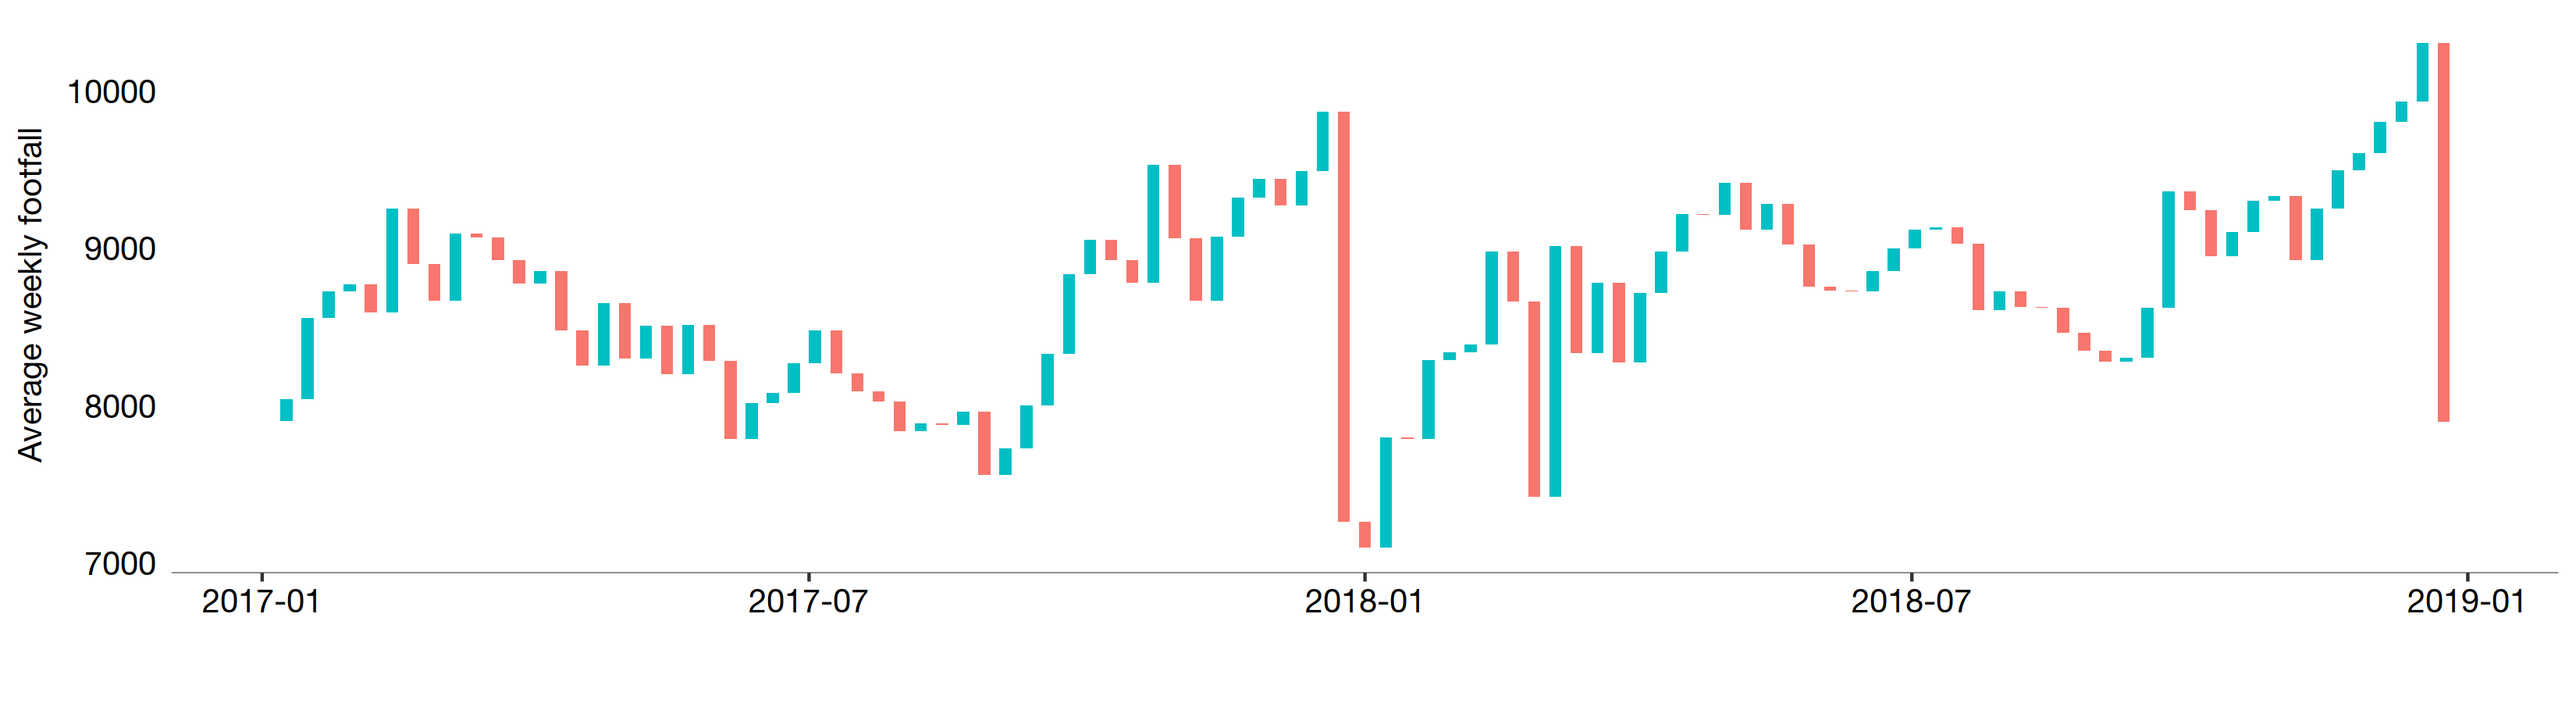
\includegraphics[trim={0 25 0 10},clip]{images/applications-footfall-index.png}
  \caption{}
  \label{}
\end{figure*}

\subsection{City wise indices}
% The footfall profiles in a day can be used to see how different cities work differently.
\lipsum[1-2]

\begin{figure*}
  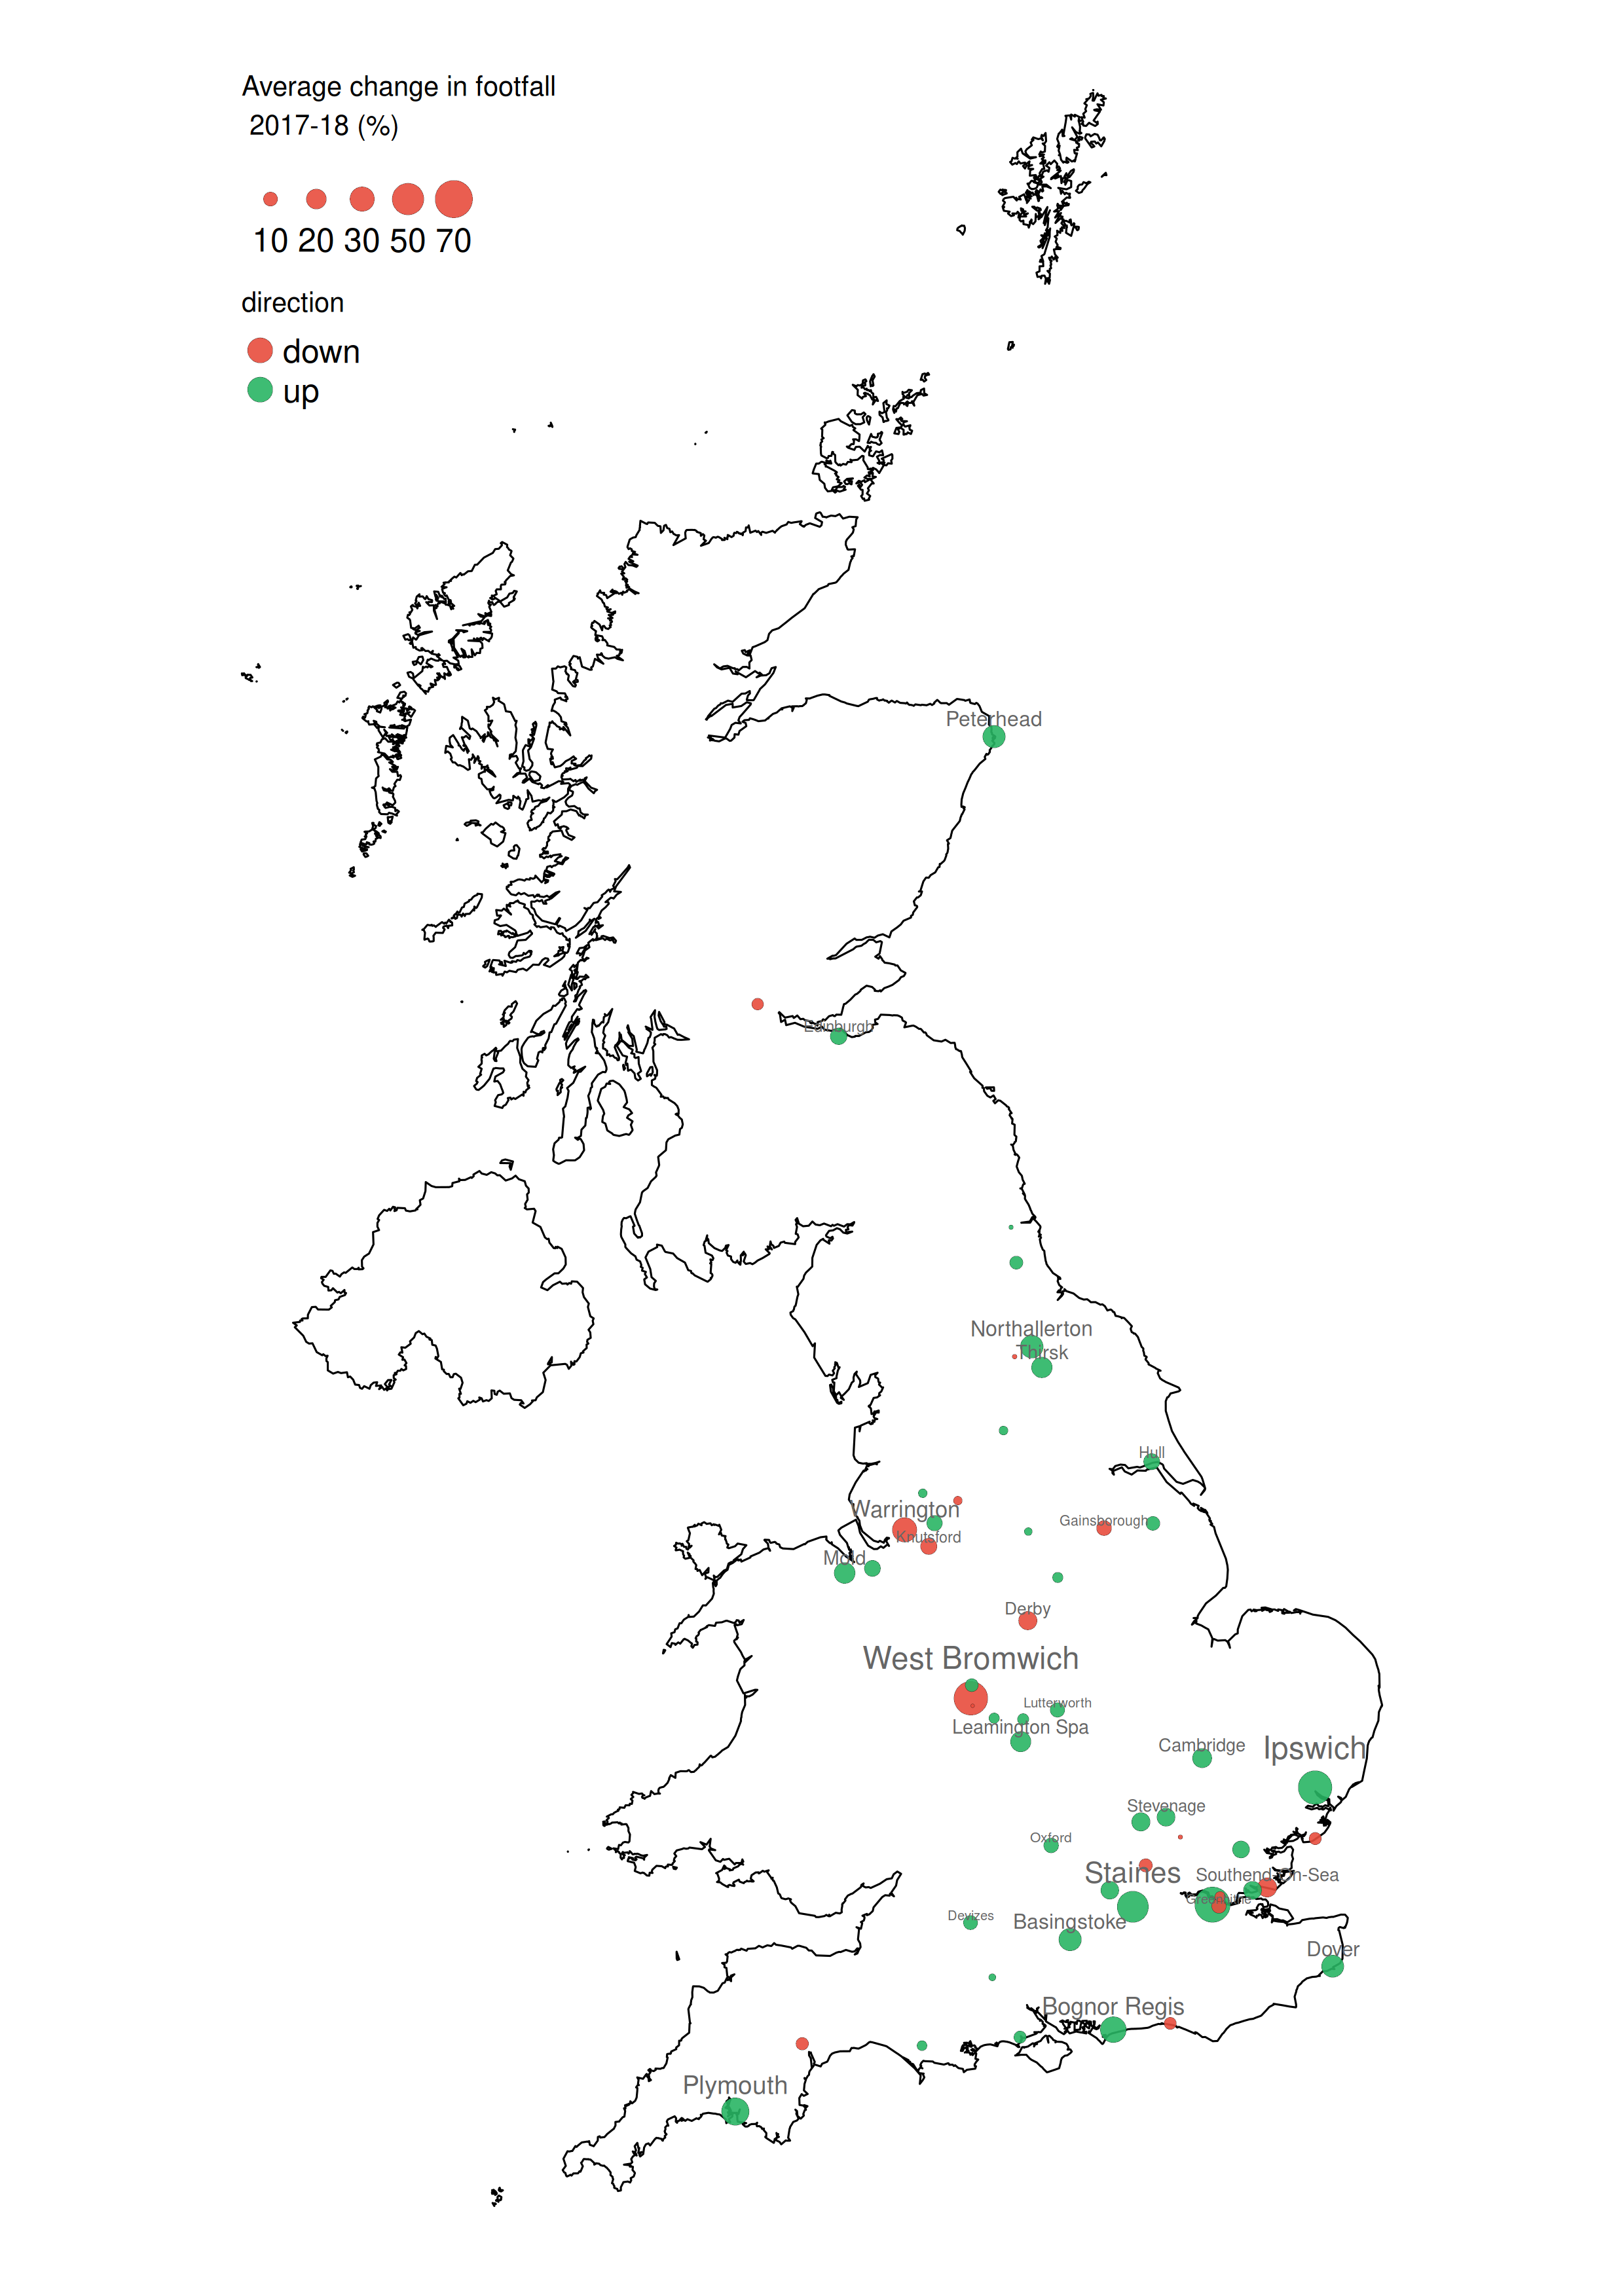
\includegraphics[trim={0 0 0 0},clip]{images/applications-cities-rank.png}
  \caption{}
  \label{}
\end{figure*}

\begin{figure*}
  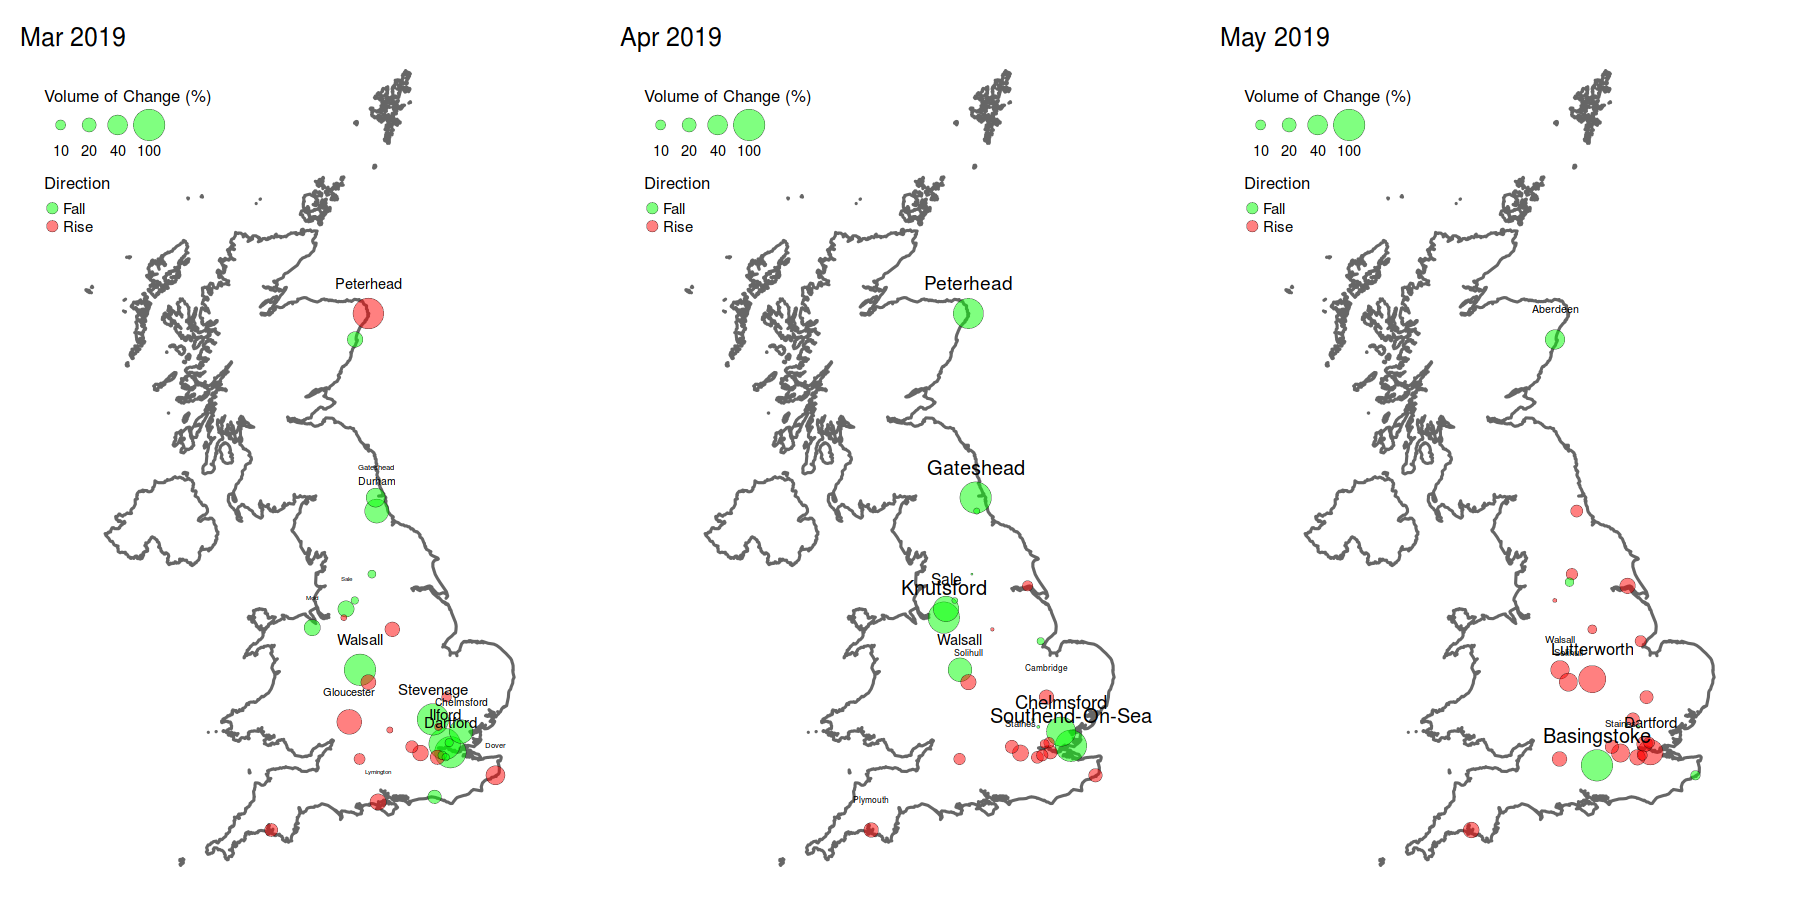
\includegraphics[trim={0 0 0 0},clip]{images/applications-city-indices.png}
  \caption{}
  \label{}
\end{figure*}

\subsection{Location comparisons}
% the locations can vary widely and their profiles can show their nature. compare couple of locations to show difference in character.
\lipsum[1]

\subsection{Longitudinal analysis}
% The profiles can be tracked longitudinally to reveal nature and change of nature over time. Footfall calendar
\lipsum[1]

\lipsum[1-2]

\cleartoleftpage
\newgeometry{
  left=20mm,
  textwidth=122mm,
  marginparsep=7mm,
  marginparwidth=43mm
}
\begin{figure*}
  \forceversofloat
  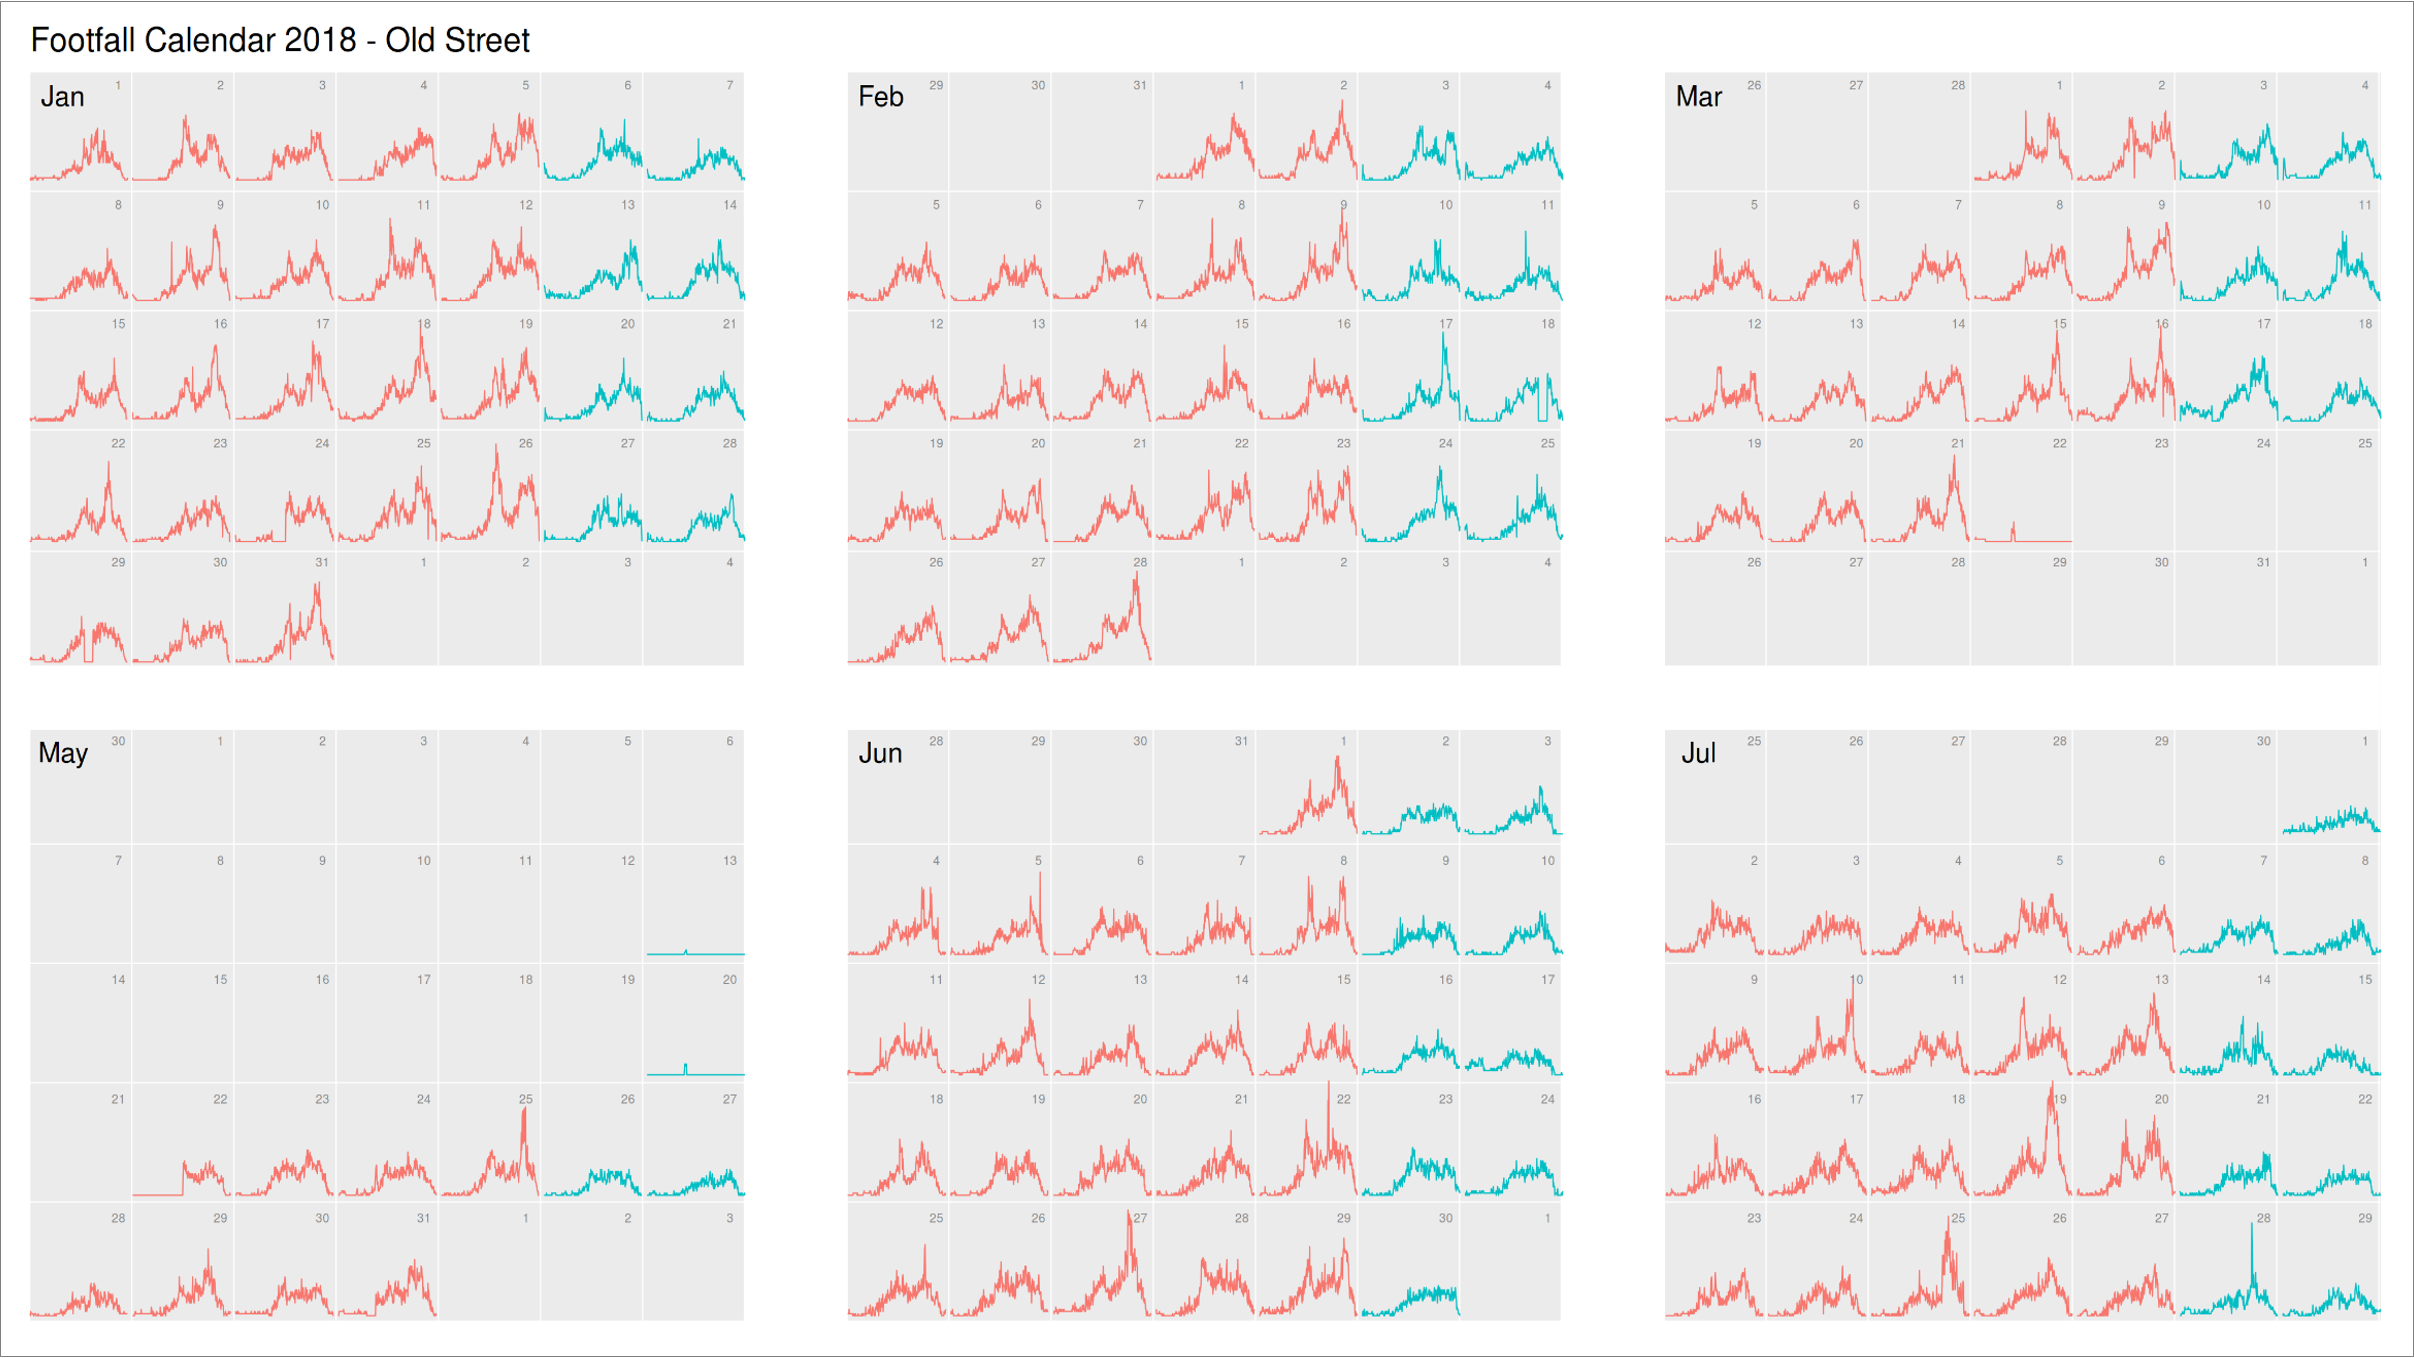
\includegraphics[width=172mm,trim={0 0 1310 -42},clip]{images/applications-footfall-calendar.png}
  \caption{Footfall calendar showing the profiles of daily volume of footfall at Old Street, London.}
  \label{}
\end{figure*}
\clearpage
\begin{figure*}
  \forcerectofloat
  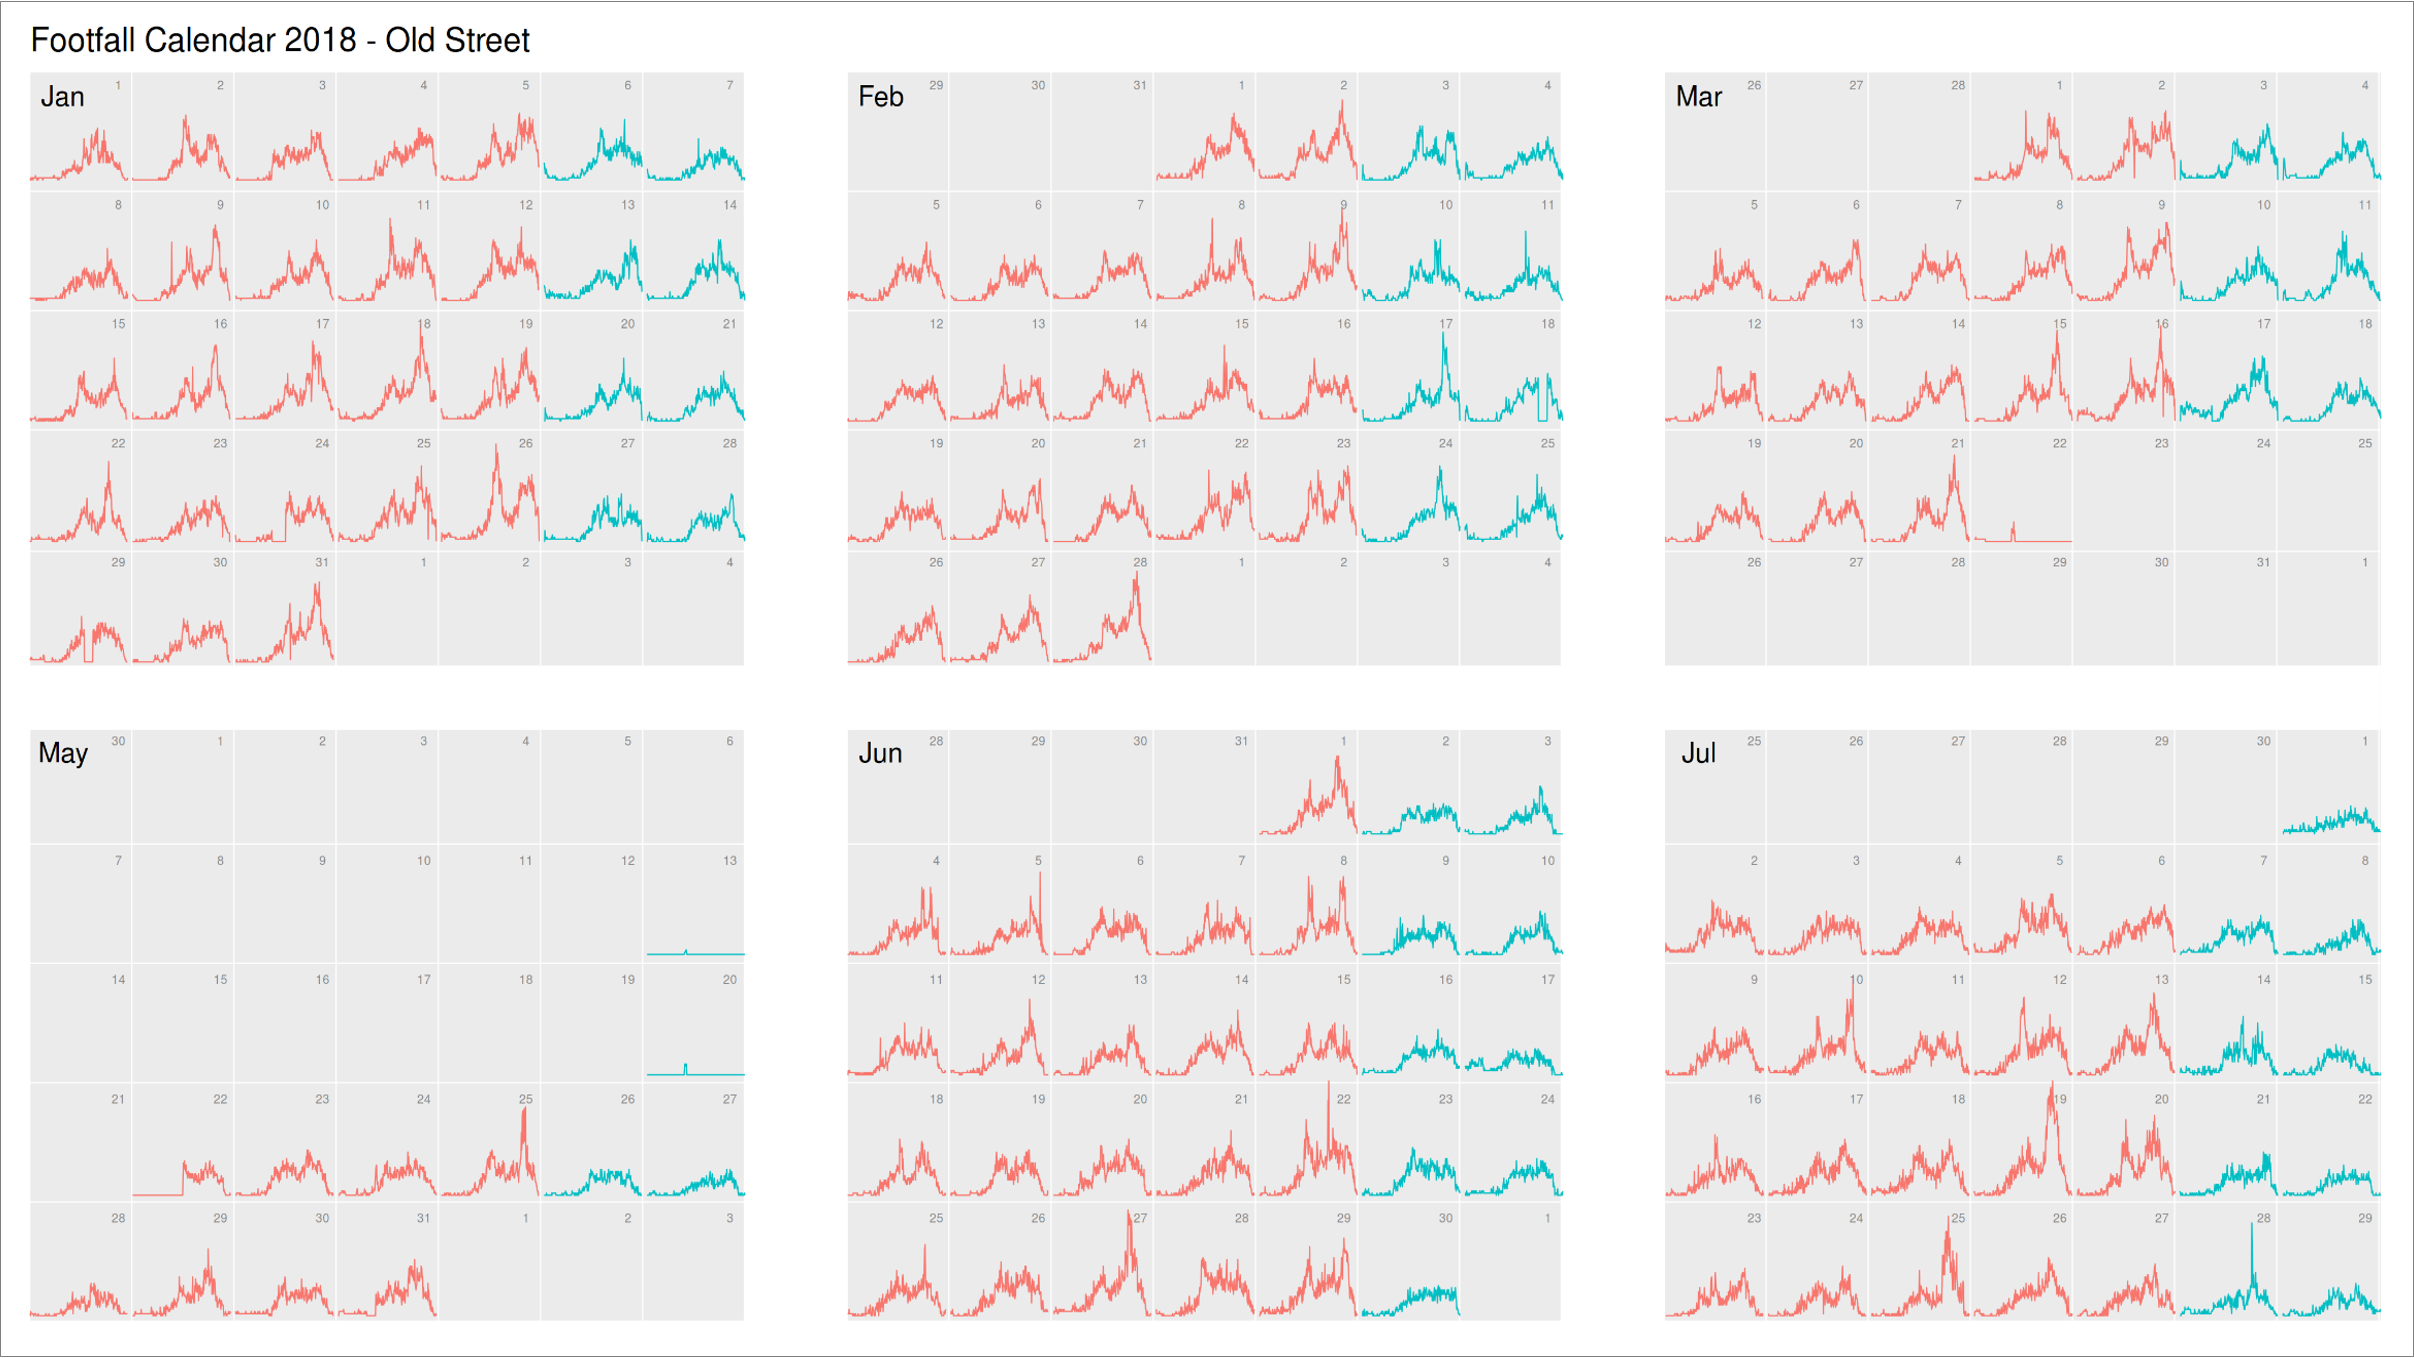
\includegraphics[width=172mm,trim={1315 0 0 0},clip]{images/applications-footfall-calendar.png}
  \caption[]{}
  \label{}
\end{figure*}
\restoregeometry
\clearpage

\lipsum[1-2]

%-------------------------------------------------------------------------------%
\section{Event Detection}
%-------------------------------------------------------------------------------%

\begin{figure*}
  \forceversofloat
  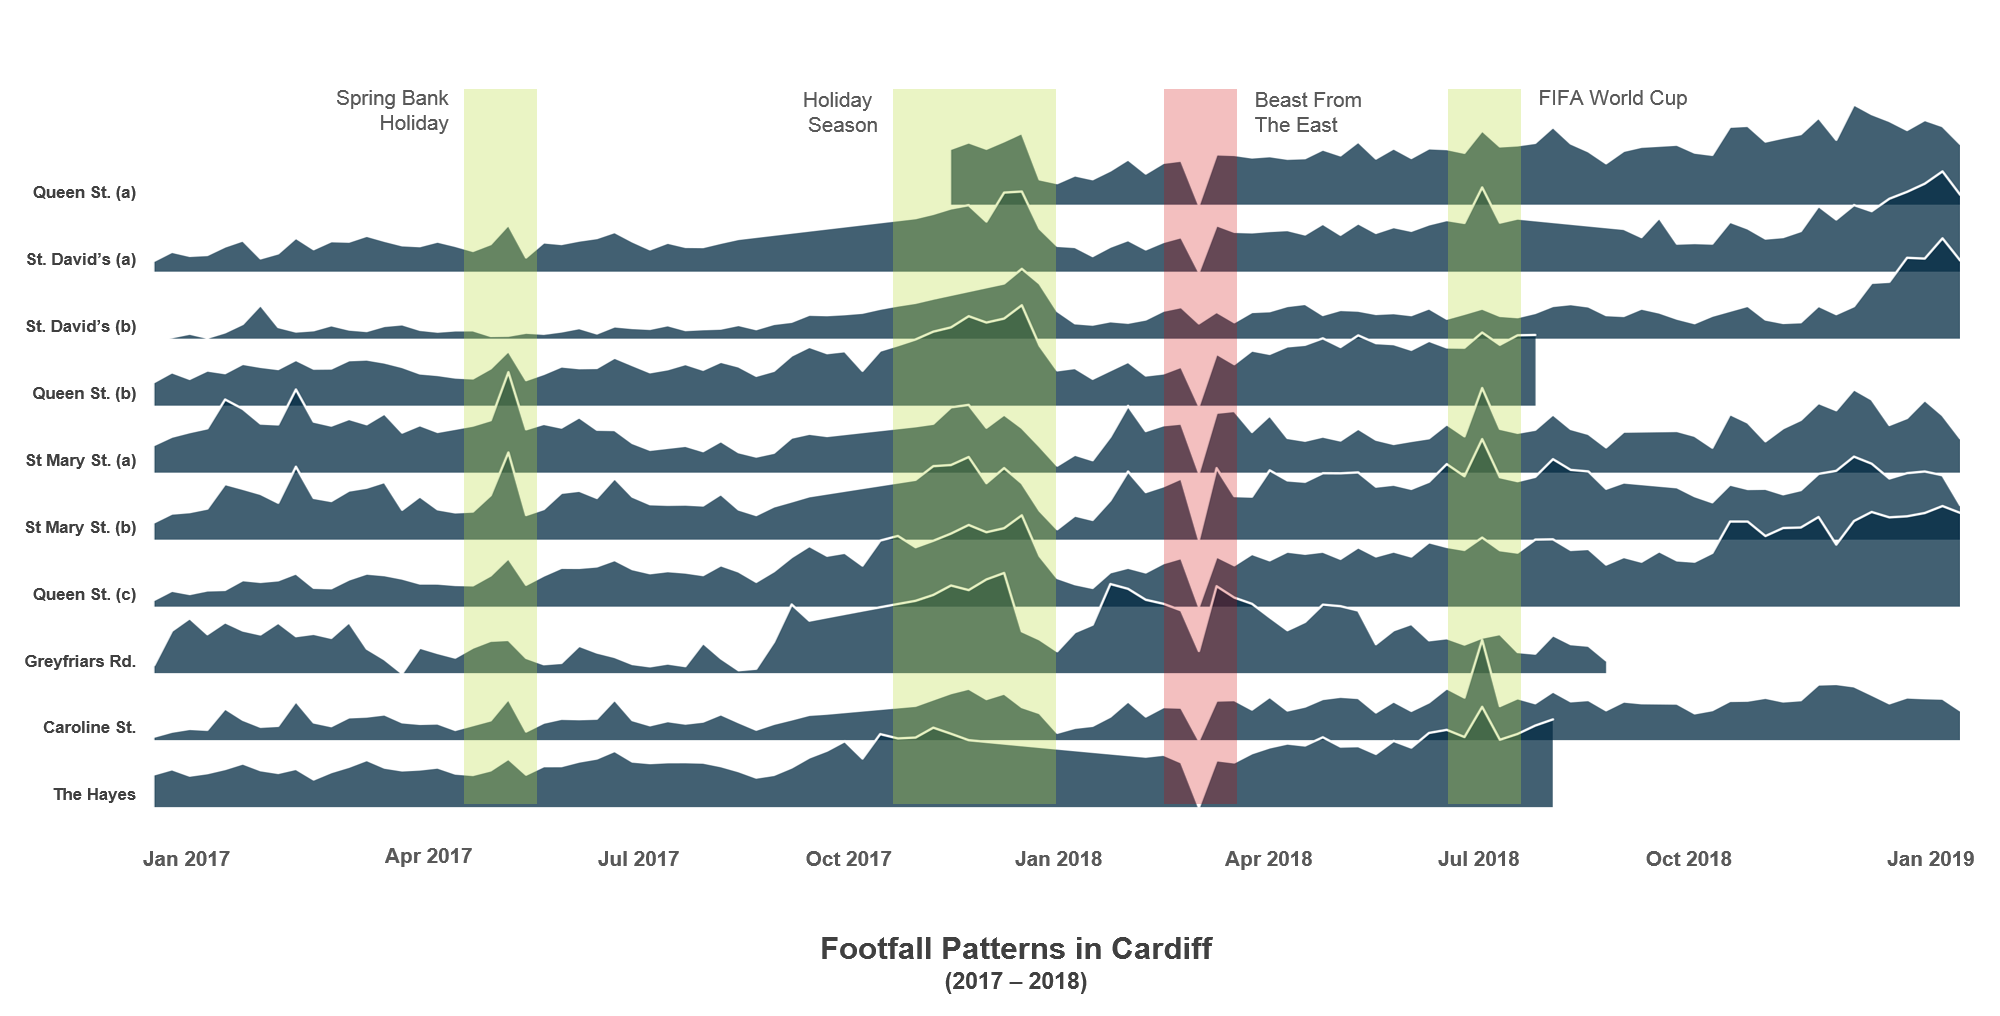
\includegraphics[trim={0 50 0 0},clip]{images/applications-cardiff-footfall.png}
  \caption{}
  \label{}
\end{figure*}

% how the data is longitudinal and can be used to detect events from the changes in footfall.
\lipsum[1]

% Discuss the events

\subsection{Football world cup}
% micro site variations could be identified as well.

% match day compared to other days.
% post match celebrations graphic.

%-------------------------------------------------------------------------------%
\section{Pedestrian Flows}
%-------------------------------------------------------------------------------%
% Tracks are a problem with this data
% But information can be extracted out of this.
% can use transfer entropy (Roberto)

\begin{figure*}
  \forceversofloat
  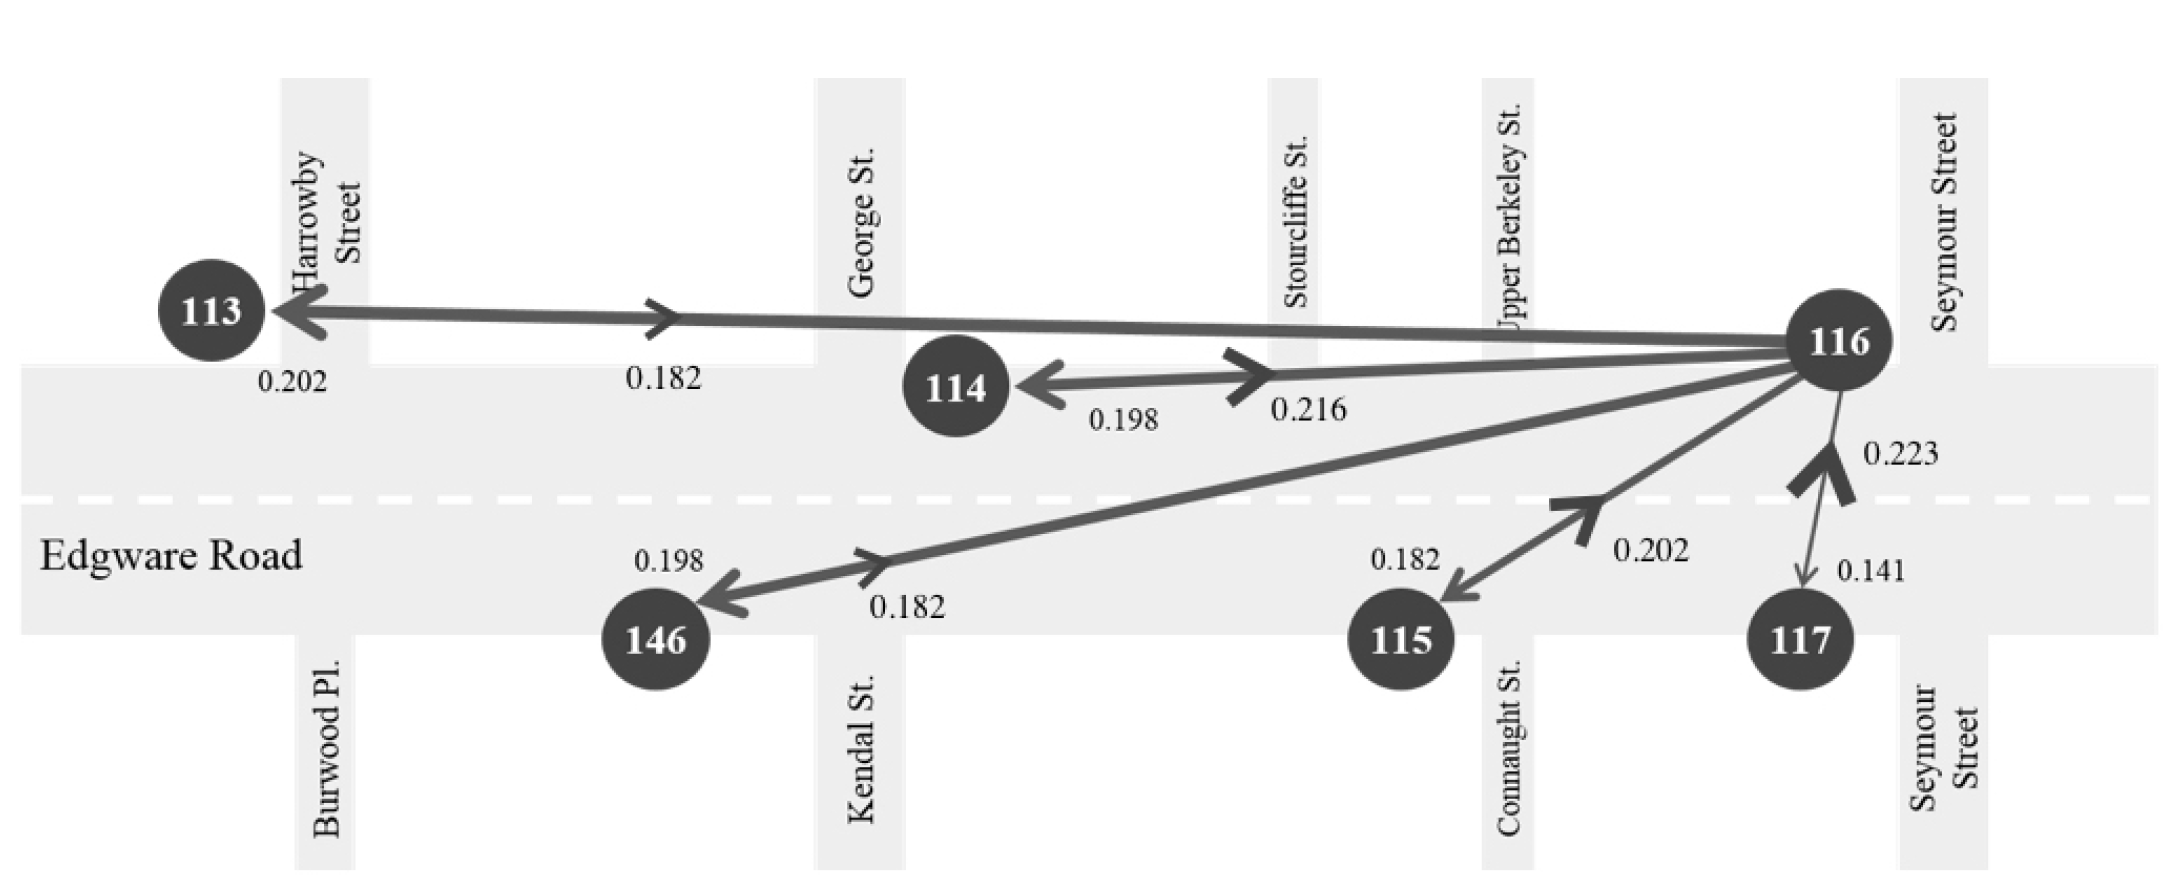
\includegraphics[trim={0 0 0 0},clip]{images/applications-transfer-entropy.png}
  \caption{}
  \label{}
\end{figure*}

% Another approach for interpolation is Geo-propagation
% It can be promising as well.

%-------------------------------------------------------------------------------%
\section{Functional Hierarchy of Places}
%-------------------------------------------------------------------------------%

% We can also understand the relationship between the places using this data.
% just using the global MAC address and how much they reoccur between the places we can infer the relationships between them and hence make a judgement of how they are organised.

% Location of 118 sensors in a map.

% network between them along with link widths.

% Hierarchy cluster map.

% Explain how the stuff works or doesn't work.

%-------------------------------------------------------------------------------%
\section{discussion}
%-------------------------------------------------------------------------------%

% 500 words on what all the above does and how it can be taken forward.
% emphasize on other work that have been done based off this data


\cleardoublepage
\chapter{Discussion and Conclusions}


\mainmatter
\cleardoublepage
\appendix
\chapter{Software}
\chapter{Code}
\addcontentsline{toc}{chapter}{Bibliography}
\bibliographystyle{apa}
\bibliography{references}





